The previous two chapters focused primarily on the performance aspects of task graph execution, by
examining various task scheduling algorithms and also bottlenecks that can limit the scalability of
existing task runtimes. However, while performance is naturally crucial for
\gls{hpc}, it should not be the only factor to focus on. \Autoref{ch:sota}
discussed several other challenges affecting \gls{hpc} task graphs that are related
to the second main focus of this thesis, namely the ergonomics of task graph execution.

This chapter deals with these ergonomic challenges through a meta-scheduling design that provides a
set of guiding principles for implementing task runtimes. It takes into account heterogeneous
resource management, fault tolerance, dynamic load balancing, interaction with allocation managers
and other aspects required to enable effortless execution of task graphs on supercomputers.

This design is then combined with the performance-related insights about task scheduling and
minimizing runtime overhead presented in Chapters~\ref{ch:estee}
and~\ref{ch:rsds} in an implementation of an \gls{hpc}-tailored task
runtime called \hyperqueue{}. This task runtime was created with the goal of enabling
transparent, ergonomic and efficient execution of task graphs on \gls{hpc} clusters.
It is the culmination of the research and work presented in this thesis, which was made possible
thanks to the experience gained from our work on \estee{} and
\rsds{}, and also from interacting with many \gls{hpc} workflows and
use-cases over the course of several years.

The work presented in this chapter makes the following contributions:
\begin{enumerate}
	\item We propose a meta-scheduling design that provides a unified way of scheduling and executing tasks
	      in the presence of allocation managers and allows load balancing across different allocations. It
	      disentangles the definition of tasks and the hardware that executes them, which makes it possible
	      to achieve high hardware utilization while also being easy to use.
	\item We provide an implementation of the meta-scheduling design in the \hyperqueue{} task
	      runtime, which enables efficient execution of task graphs on heterogeneous \gls{hpc}
	      clusters. It also supports dynamic load balancing features that are not present in other
	      state-of-the-art tools, such as fractional resources and resource variants.
	\item We evaluate the performance, scalability and achieved hardware utilization of task graphs executed
	      using \hyperqueue{} on several benchmarks and use-cases.
\end{enumerate}

This chapter first introduces the proposed general meta-scheduling design. Then it describes the
architecture of \hyperqueue{}, which implements the proposed design, and presents how its
features alleviate the challenges described in~\Autoref{ch:sota}. Finally, it presents
several use-cases where \hyperqueue{} was successfully used, provides a performance
analysis of \hyperqueue{} on various stress tests and compares it with state-of-the-art
meta-scheduling task runtimes.

We have described the design and key ideas of \hyperqueue{} in
\emph{HyperQueue: efficient and ergonomic task graphs on HPC clusters}~\cite{hyperqueue}. The architecture of \hyperqueue{}
presented in this chapter was adapted from this publication.

\workshare{I have collaborated on this work with Ada Böhm; we have both contributed to it equally. I am the
sole author of the design and implementation of the automatic allocator
component, and I have also significantly contributed to the design and implementation of most remaining parts
of \hyperqueue{}. I have designed and performed all the experiments described in this
chapter. While Ada and I are the primary contributors to \hyperqueue{}, it should be noted that other people have also contributed to it, as its development is a team effort. Source code contribution statistics for
\hyperqueue{} can be found on GitHub\footnoteurl{https://github.com/it4innovations/hyperqueue/graphs/contributors}.}

\section{Meta-scheduling design}
This section describes a design for executing task graphs that aims to alleviate the challenges
described in~\Autoref{ch:sota}. First, a general overview of the design will be introduced,
and the following sections will then describe its concrete implementation within the
\hyperqueue{} task runtime. The design consists of a set of general guidelines that help
drive the design of task runtimes so that they will be able to resolve the mentioned challenges.
Note that there are some task runtime aspects, such as simple deployment or high runtime
efficiency, that have to be resolved with specific implementation choices, rather than general
principles. These will be mentioned in the next section that details the implementation of
\hyperqueue{}. This section focuses on more general principles that do not depend that
much on a specific implementation.

The primary challenge that affects the simplicity of task graph execution on
\gls{hpc} clusters is the presence of an allocation manager, because it forms a
barrier; on such clusters, it is not possible to compute anything at all without interacting with
allocations. In order for task graph execution to become truly ergonomic, it is the first and
foremost challenge that needs to be resolved. It is also tied to most of the other mentioned
challenges; heterogeneous resource requirements, fault tolerance and efficient hardware utilization
on supercomputers are all affected by the way the task runtime handles allocations. It will thus be
the main focus of the described guidelines.

\Autoref{challenge:allocation-manager} has described several approaches that can be used to map tasks to
allocations, which is necessary to execute task graphs, as well as their various shortcomings. Due
to the limits imposed by allocation managers, it might be necessary to partition task graphs into
multiple subgraphs in order to fit them within an allocation, which can be challenging.
Furthermore, it can result in non-optimal usage of hardware resources, because tasks from
(sub)graphs submitted in separate allocations will only be load balanced within their own
allocation, and not across different allocations.

It is important to note what is uniquely challenging about the interaction with allocations. The
fact that the computation needs to go through a queue is not an issue by itself, as we are dealing
with batch processing anyway. Therefore, some form of a delay between submitting the task graph and
receiving the results is expected, even if we did not have to submit allocations at all.

The main issue of allocations is that they strictly tie together two separate aspects;
\emph{what} the user wants to compute (the computation performed once the allocation
starts) and \emph{where} should the computation take place (specific hardware resources
and computational nodes reserved for the allocation). As was already described previously, both of
these things have to be specified together in an allocation. This is a very inflexible design, for
several reasons:

\begin{itemize}
	\item The user needs to consider both aspects at the same time. Ultimately, the main thing that the user
	      cares about is what they want to compute. With allocations, they also need to think about specific
	      hardware resources that should be allocated for computing their tasks, and how should tasks be
	      mapped to these resources, which can be challenging.
	\item Hardware resources are allocated for the whole duration of the allocation. This can result in
	      inefficient resource usage, especially for heterogeneous task graphs that consist of many types of
	      tasks that use different resources. In situations where not all resources can be used at the same
	      time, some of the resources can unnecessarily remain idle.
	\item The amount of used resources has to be decided up front, and new hardware resources cannot be added
	      or removed from existing allocations. Apart from the potential resource waste, this can also limit
	      load balancing. If load balancing only happens within (and not across) allocations, then resources
	      from different allocations cannot be pooled together to make the task graph execution faster, and
	      users also cannot easily provide new hardware resources during the computation.
	\item Granularity of the allocated resources might not match the granularity of tasks. Unless the
	      allocation manager supports very fine-grained allocations (e.g.\ on the level of individual
	      \gls{cpu} cores, rather than whole computational nodes), there can be a large gap
	      between the resources required by a task graph and the resources provided to an individual
	      allocation. This can again lead to resources sitting idle.
	\item Binding computation with specific hardware resources up front complicates handling task failures.
	      When the user submits thousands of tasks on a specific set of hardware resources, and some of these
	      tasks fail, the user might need to create a new allocation to recompute the failed tasks. This
	      requires once again figuring out a new set of hardware resources that should be requested, as the
	      original resources will probably not be a good fit for just a subset of the original computation. A
	      fault-tolerant design would ideally allow recomputing tasks on any compatible hardware resource
	      transparently, which is incompatible with forcing computations and resources to be defined
	      together.
\end{itemize}

As an aside, it is interesting to note that some of these challenges uniquely affect task graphs,
and in general programming models that are different from the traditional ways of defining
\gls{hpc} computations. Consider a distributed application implemented using
\gls{mpi}, which has historically been a common way of defining computations on
supercomputers. \gls{mpi} applications typically assume that they will run on a set
of computational nodes for a relatively long duration (hours or even days). This set of nodes
(corresponding to \gls{mpi} processes) usually does not change during the
computation; it is not trivial to add new processes, and if some of the processes crash, it
typically leads to the whole computation being aborted, as fault tolerance is not a default
property of \gls{mpi} applications~\cite{fault_tolerant_mpi}.

These properties of \gls{mpi} applications are similar to the mentioned properties of
allocations, so they fit together well, and using allocations to execute them is relatively
straightforward. In fact, it is clear that the allocation model itself was designed with
\gls{mpi}-like use-cases in mind. Therefore, it is not very surprising that the
concept of allocations is not a good match for programming models that are very different from
\gls{mpi}, such as task-based workflows.

We can make an observation that the most problematic aspect of allocations is their requirement to
define computations and hardware resources together. The key idea of the proposed meta-scheduling
design is thus to completely disentangle the definition of what the user wants to compute (tasks)
from the hardware resources where the computation should take place (computational nodes,
\gls{cpu} cores, etc.). By separating these two concerns, we enable users to focus on
what they care about the most (their task graphs), instead of having to think about mapping tasks
to allocations and graph partitioning.

In order to disentangle these two concepts, we have to rethink what kind of computation is
submitted in allocations. Instead of making allocations execute tasks or task graphs directly, they
should execute generic computational providers, which will then be dynamically assigned work (tasks
to execute) based on the current computational load. This both improves the achievable hardware
utilization and simplifies the allocation submission process. The following principles describe a
meta-scheduling approach based on this idea.

\begin{description}[wide=0pt]
	\item[Task runtime runs outside of allocations] In order to allow fully dynamic load balancing, the task runtime should not be tied to a specific
		allocation. Instead, it should run at some persistent location of the cluster (e.g.\ on a login
		node). This enables users to submit tasks to it independently of allocations, which is a crucial
		property. This removes the need to decide which tasks should be computed on which concrete hardware
		resources and in which allocations up front. It can also help improve hardware utilization, because
		it provides the task runtime the possibility to load balance tasks across all active allocations.

		This is where the term \emph{meta-scheduling} comes in; the essence of the idea is to use a task
		runtime as a sort of high-level scheduler on top of an allocation manager. Instead of forcing users
		to think in terms of allocations, they can submit task graphs in the same way they would on a
		system that is not supervised by allocation managers, and let the task runtime automatically decide
		in which allocation a task should be executed.

		With this approach, the task runtime will most likely run in an environment that is shared with
		other users of the cluster, rather than being executed inside secured and isolated allocations. It
		should thus offer its users an option to encrypt its communication to avoid other users of the
		cluster reading sensitive data, e.g.\ task outputs sent from workers.
	\item[Allocations are uniform] Even with the task runtime running outside an allocation, it is still necessary to submit
		\emph{some} allocations to provide hardware resources that will actually execute tasks.
		Instead of defining specific tasks that should be computed within an allocation, allocations should
		execute a generic computational provider (worker) that will be assigned tasks to execute
		dynamically by the task runtime. This assignment can happen e.g.\ by a centralized component
		pushing tasks to workers over the network, or by the workers pulling work from a queue or a
		distributed database.

		With this approach, allocations become trivial and completely uniform, because they all have the
		same structure; each allocation simply starts a (set of) computational provider(s). This makes it
		much easier for users to submit allocations. Instead of thinking about how to partition their task
		graphs, users simply decide how many computational resources they want to spend at any given
		moment, and start the corresponding number of allocations.
	\item[Allocations are submitted automatically] A corollary of the previous principle is that it becomes possible to submit allocations fully
		automatically by the task runtime. It can use its knowledge of the current computational load to
		submit workers whose resources would help execute tasks that are currently submitted. This removes
		saves users from performing a laborious manual process (allocation submission) and can further help
		improve hardware utilization, since the task runtime can use its knowledge to dynamically increase
		and decrease the number of active workers.
	\item[Failed tasks are retried automatically] Once allocations become generic computational providers, their lifetime is no longer bound to a
		specific set of tasks. And since allocations will often end abruptly, they might disappear in the
		midst of a task being computed. This is not a failure of the task per se; it is a mostly
		unavoidable consequence of allocations being transient. Such tasks should thus be automatically
		reassigned by the task runtime to a different worker without the user's intervention, to ensure
		uninterrupted execution of the task graph.

		The fact that the task runtime resides outside of allocations further facilitates fault tolerance,
		because an allocation failure will not affect the state of tasks stored in the task runtime. In
		order to also be resilient against e.g.\ login node failures, the task runtime should be able to
		restore its state from persistent storage (e.g.\ a filesystem or a database).
	\item[Dependencies are independent of allocations] The allocation manager should not act as a task runtime and thus it should not handle dependencies
		between tasks. These should be expressed solely on the level of the task runtime itself, and they
		should be fully independent of allocations. This approach also facilitates execution of the task
		runtime on a local computer, where there most likely will not be any allocation manager.
	\item[Tasks are paired with workers using abstract resources] The first two principles described above separate the two core pillars of task graph execution; the
		definition of the task graph and the provisioning of hardware resources. However, it is in fact
		required to somehow tie these two aspects together, because tasks can have resource requirements
		that constraint the environment in which they can be executed.

		We saw that submitting tasks directly as allocations, which explicitly ties tasks to a set of
		hardware resources, had many disadvantages. Instead, the task runtime should provide a resource
		system that will allow users to pair tasks with workers in a general and abstract way. Each task
		can describe a set of abstract resources that have to be available so that the task can be
		executed, and each worker will in turn provide a set of abstract resources that it provides. The
		task runtime will then dynamically assign tasks to workers by matching these resources together,
		while making sure that worker resources are not being oversubscribed.

		Crucially, this approach allows users to avoid considering the granularity of hardware resources
		provided in allocations. Even if the allocation manager always provides at least a whole node in
		each allocation, multiple granular tasks (even from completely independent task graphs) that
		require e.g.\ only a single core can be load balanced onto that same node.

		Furthermore, it should be possible to define custom kinds of resource requirements, to support
		heterogeneous clusters that might have arbitrary hardware resources, such as special accelerator
		devices or network interconnects.

		It is also important to make sure that resource genericity does not hinder efficiency. The task
		runtime should provide a generic way to express common resource patterns, such as a task that
		requires \gls{cpu} cores residing in the same \gls{numa} node.
\end{description}

This set of guidelines should enable execution of heterogeneous task graphs on supercomputers in a
straightforward way. Thanks to sidestepping the allocation manager by moving the task runtime
outside of allocations, we can sidestep the limits associated with executing tasks in allocations
directly, such as limited support for dependencies, limited scale of task graphs that can be
executed, and non-optimal load balancing and hardware utilization. In combination with a generic
resource system, automatic allocations and automatic re-execution of failed tasks by default, this
design should provide an ergonomic experience for task graph authors.

Of course, as with any approach, there are certain trade-offs associated with these guidelines. For
example, running the task runtime on a login node might be problematic if the login nodes are
severely computationally constrained or if they are not even able to connect to compute nodes of
the \gls{hpc} cluster through the network. Performance and security aspects of this
deployment method also need to be considered.

These trade-offs will depend on a specific implementation of a task runtime that will leverage the
described guidelines. To evaluate how the proposed approach works in practice, what its performance
and usage implications are and how it compares to existing meta-schedulers, we have implemented
this general design in a task runtime called \hyperqueue{}, which will be described in
the rest of this chapter.

\section{\hyperqueue{}}
\hyperqueue{} (\hq{}) is a distributed task runtime that aims to make task graph execution a
first-class concept on supercomputers. It does that by implementing the meta-scheduling design
described in the previous section and leveraging insights gained from our task scheduling
experiments and \dask{} runtime efficiency analysis. In terms of architecture and
implementation, it is an evolution of the \rsds{} task runtime described
in~\Autoref{ch:rsds}; however, instead of using the \dask{} components and
\glspl{api}, it implements its own task-based programming model.
\hyperqueue{} is developed in the Rust programming language~\cite{rust} and
it is provided as an \mbox{MIT-licensed} open-source tool~\cite{hq_github}.

This section describes the high-level design of \hyperqueue{}, its programming model and
the most important features. It also presents several use-cases where it has been successfully
leveraged, and evaluates its performance and other aspects in various experiments.

Note that for simplicity, Slurm will be used as a default representative of an allocation manager
throughout this whole chapter, but it could be replaced by \gls{pbs} or any other
commonly used allocation manager without loss of generality.

\subsection{Architecture}
\label{hq:architecture}
\hyperqueue{} uses a fairly standard distributed architecture. It consists of two main
components, a central management service called a \emph{server} and a component that
serves as a computational provider which executes tasks, called a \emph{worker}. Users
then interact with the server using a \emph{client} interface.~\Autoref{fig:hq-architecture}
displays a high-level view of the \hq{} architecture for a typical deployment on
an \gls{hpc} cluster with an allocation manager, where the server runs on a login
node and meta-schedules tasks to workers that run on computational nodes in various allocations.
The individual components are described in more detail below.

\begin{figure}[h]
	\centering
	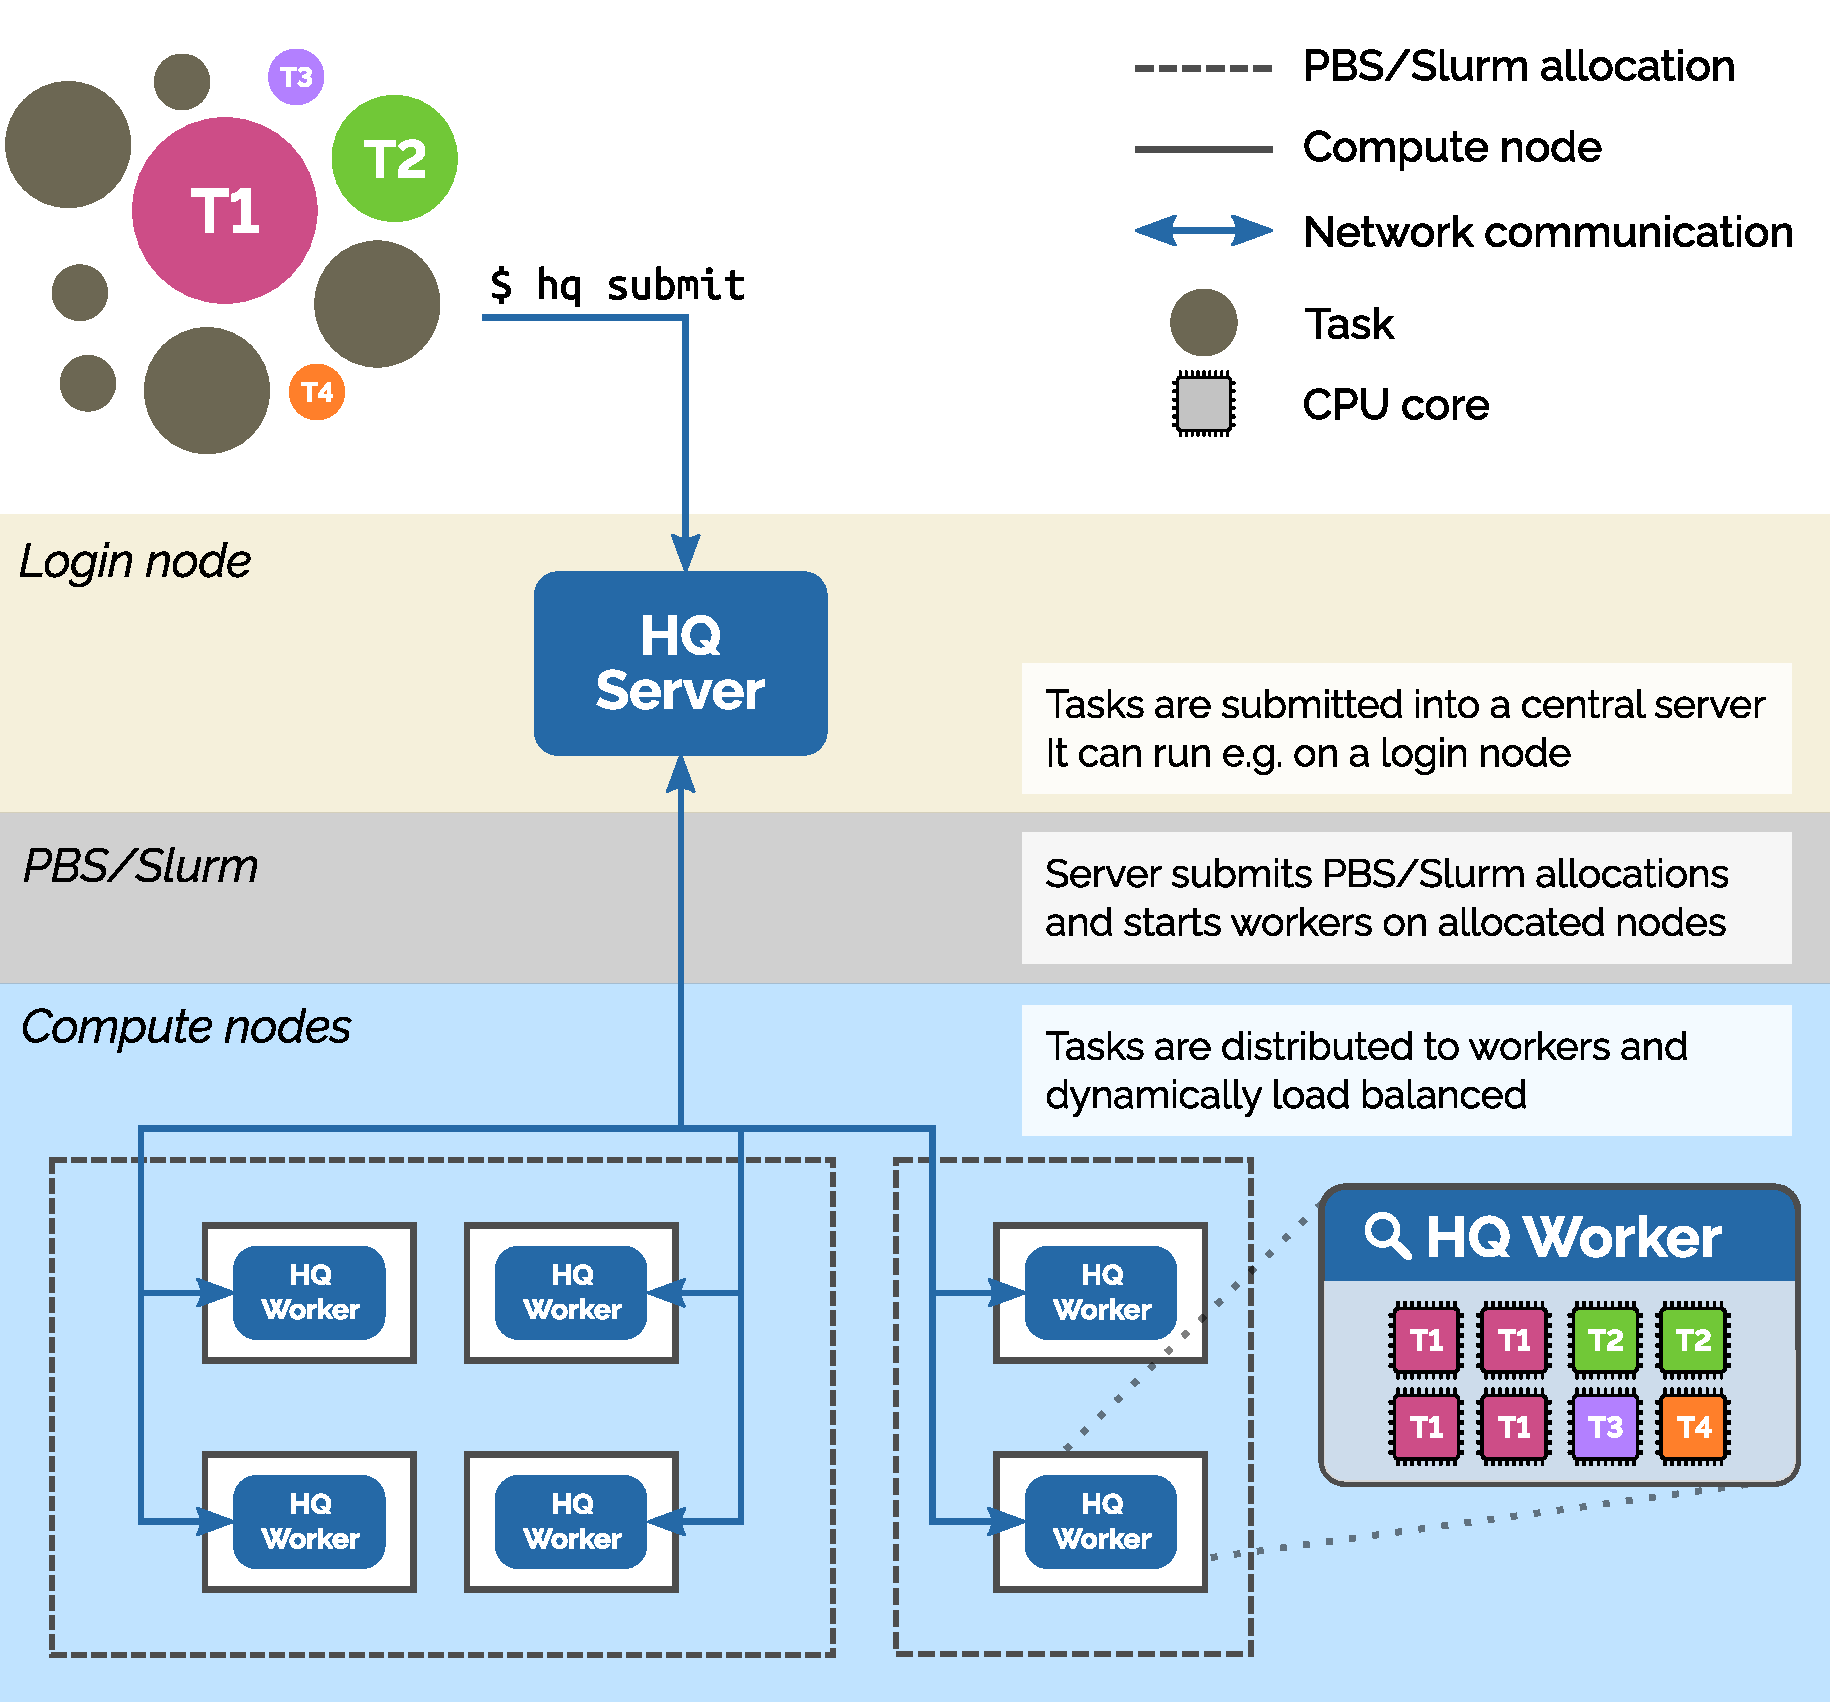
\includegraphics[width=0.7\textwidth]{imgs/hq/architecture}
	\caption{Architecture of \hyperqueue{}.}
	\label{fig:hq-architecture}
\end{figure}

\subsubsection*{Server}
The \emph{server} is the most important part of \hyperqueue{}. Its main goal is
to manage both the lifecycle of task graphs and of workers that provide computational resources. It
keeps track of all tasks and workers, and allows users to query their state and also send commands
to it through a client interface. The server contains a work-stealing task scheduler that is based
on the \rsds{} scheduler implementation described in~\Autoref{sec:rsds-description}. The
scheduler assigns individual tasks to workers based on task resource requirements and current
computational load of workers, with the goal of maximizing hardware utilization of the connected
workers.

It is designed to be executed as a long-running background process, which should ideally be
executed in a persistent location not managed by allocation managers (i.e.\ outside ephemeral
allocations). Typically, it is executed on a login node of a cluster, but it can also run
elsewhere, for example in a cloud partition. It should keep running until all tasks that the user
wants to execute are finished, although it can also restore its state from disk, so the computation
of a task graph can be interrupted and resumed at a later time, if needed.

The fact that the server runs outside allocations allows it to load balance tasks across workers
running in multiple allocations concurrently, and work around the various limits of allocation
managers. This adheres to the first principle of the meta-scheduling design described in the
previous section.

The server itself does not execute any tasks, and it consumes a relatively modest amount of
resources, and therefore it is not computationally demanding.~\Autoref{sec:hq-exp-server-cpu-consumption} evaluates how
many \gls{cpu} resources the server consumes in extreme scenarios.

Apart from basic responsibilities related to worker management and task scheduling, the server also
provides additional functionality. For example, it can submit allocations fully automatically on
behalf of the user. This feature will be described in detail in~\Autoref{hq:automatic-allocation}.

The inner architecture of the server is displayed in~\Autoref{fig:hq-server-architecture}. The server is divided
into two parts; frontend and backend. The frontend part is responsible for managing a database of
task graphs and workers and providing access to it to clients. It also stores all important events
(such as a task being completed or a task graph being submitted) into a journal file, from which it
can restore its state in case of an unexpected failure. The frontend also runs the automatic
allocator, which submits allocations into Slurm or \gls{pbs} to spawn new workers.

\begin{figure}[h]
	\centering
	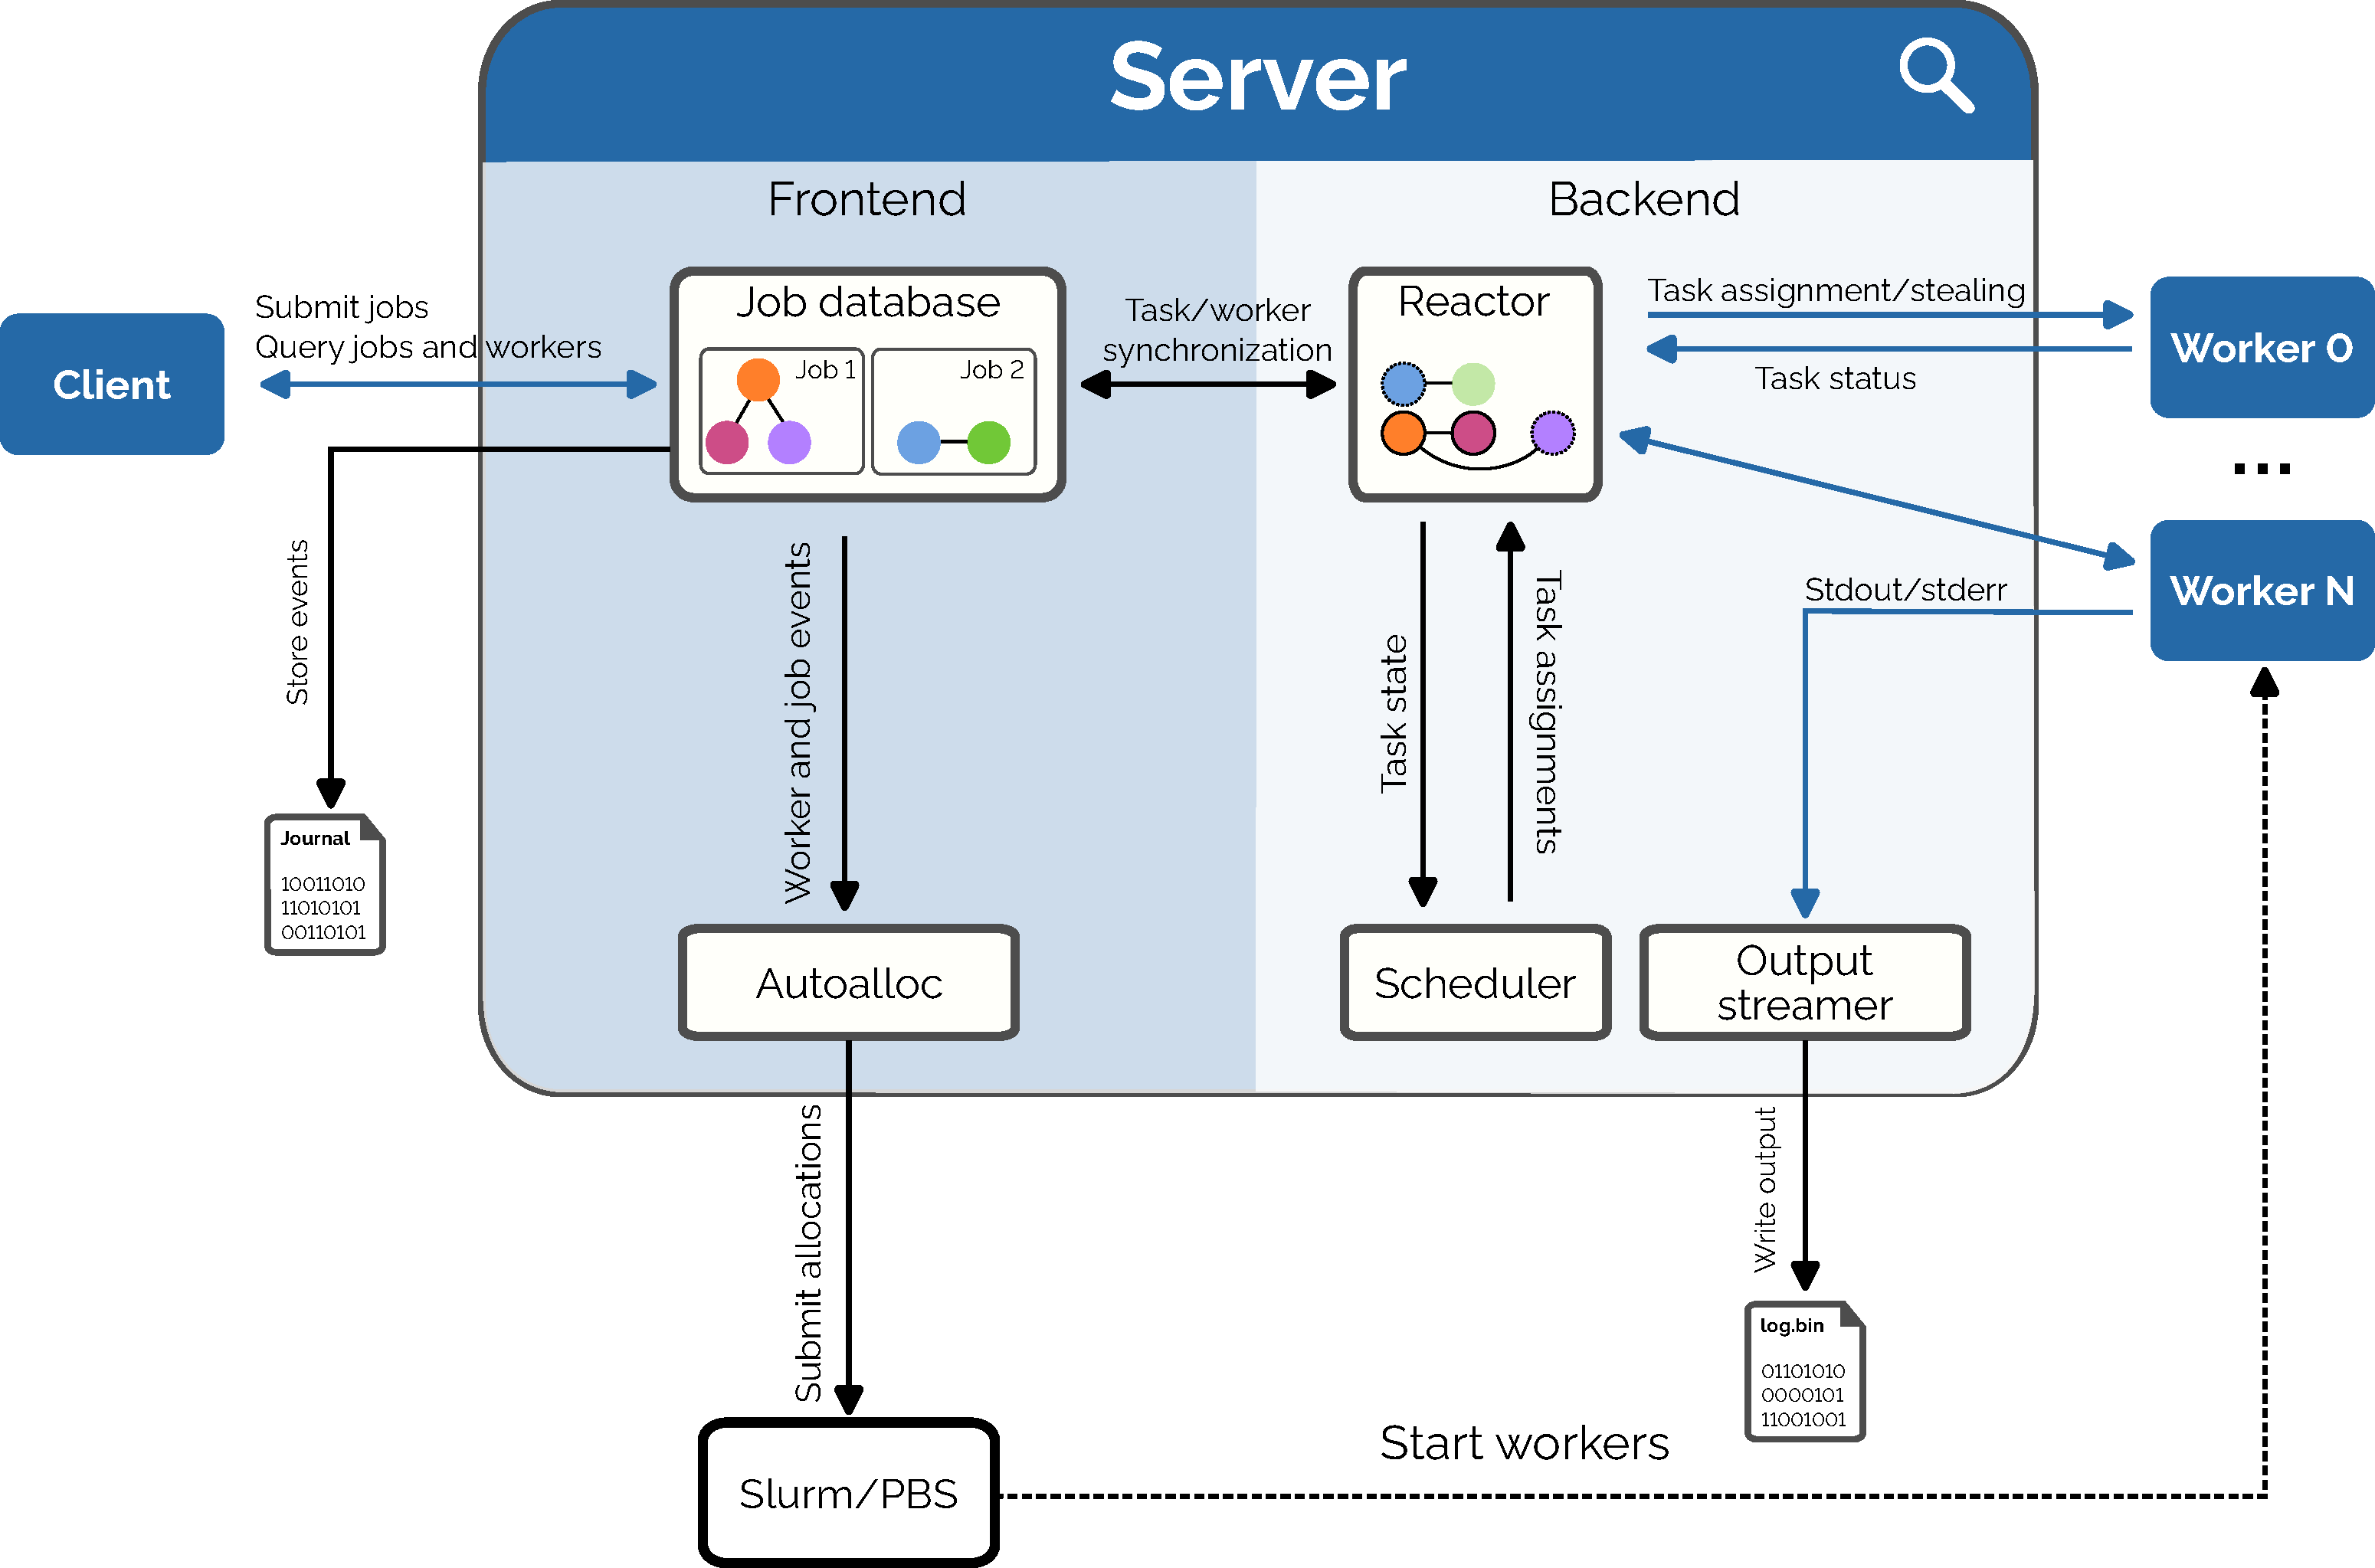
\includegraphics[width=0.9\textwidth]{imgs/hq/server-architecture}
	\caption{Architecture of the \hyperqueue{} server.}
	\label{fig:hq-server-architecture}
\end{figure}

The backend is the performance-critical part of the server. It does not separate individual task
graphs submitted by users, it simply works with a bag of tasks that it schedules to workers. It
passes task updates to a separate scheduler component that computes the assignments of tasks to
workers using the \emph{b-level} heuristic and work-stealing (this implementation is based
on the \rsds{} scheduler). It then sends the assigned tasks to individual workers
and processes task results from them. The backend also contains a component for streaming standard
(error) output generated by tasks from workers into binary files, which can be used to avoid
putting too much stress on distributed filesystems. This will be described
in~\Autoref{hq:task-input-and-output}.

Even though both parts (frontend and backend) currently run inside the same Linux process, they are
strictly separated and communicate together using a well-defined interface. Therefore, it would be
possible to deploy the backend in a separate process or even run it on a different node, in which
case the two parts would communicate over the network. This could be useful for example to run the
backend on a more powerful computational node.

\subsubsection*{Worker}
The \emph{worker} component is a computational provider that executes tasks assigned to
it by the server. A single worker typically manages all hardware resources (\gls{cpu}
cores, \gls{gpu} or \gls{fpga} accelerators, memory, etc.) of a given
computer, usually a single computational node of a supercomputer.

The worker is able to automatically detect all relevant hardware resources that are available on
the node where it is started and advertise them to the server. Therefore, in a typical case, users
can simply start the worker on a given node with a single uniform command, and from that moment on
the resources of that node will be used for task execution. This adheres to the second principle of
the proposed meta-scheduling design, where computational providers should be generic (not tied to
any specific task or a set of tasks), and it should be possible to start them using a uniform
command, to make their deployment trivial.

Each worker also participates in task and resource scheduling. The server makes high-level
scheduling decisions, such as which tasks will be executed on a given worker, while the worker then
performs micro decisions, such as in which order it will execute tasks assigned to it, or which
specific resources will be assigned to a given task. Resource management will be described in more
detail in~\Autoref{sec:hq-resource-management}.

\hyperqueue{} workers were designed with fault tolerance in mind. On an
\gls{hpc}
cluster, workers will be typically executed inside allocations that only run for a limited amount
of time, which implies that workers can disappear at any time during the computation of a task
graph. Both the server and workers thus operate with the assumption that workers can be potentially
short-lived; if a worker disconnects while it is executing a task, the task will be transparently
reassigned to a different worker without user intervention. Worker management is thus dynamic and
flexible; new workers can also be added at any time, after which they will immediately start
contributing to the execution of the submitted task graphs. This property enables users of
\hq{} to arbitrarily scale the computation of a task graph both up and down, even
while it is being executed, by dynamically adding or removing workers as needed.

While workers can be deployed manually by users, \hq{} can also automatically
submit allocations to an allocation manager that start workers on computational nodes, based on
current computational needs of submitted task graphs, as was already mentioned. This system, called
\emph{automatic allocation}, will be described in more detail later in~\Autoref{hq:automatic-allocation}.

\subsubsection*{Client interfaces}
Users can use two main interfaces for deploying the \hyperqueue{} server and workers,
submitting task graphs and managing and monitoring the computation. They can either use a
\gls{cli}, which has been designed to feel familiar to users of Slurm in order to
make it easier to migrate existing \gls{hpc} workflows to \hyperqueue{}, or
a Python \gls{api}, which is useful for more complex use-cases that are challenging
to express using the command line. These interfaces are relatively large, and their specific shape
is not crucial for this thesis; the complete set of the supported \gls{cli} commands
and their parameters and the Python \gls{api} is described in the
\hyperqueue{} documentation~\cite{hq_docs}. In the rest of the text, we will
show various examples of these interfaces (primarily of several \gls{cli} commands),
to provide an idea of how ergonomic it is for users to interact with \hyperqueue{}.

The \gls{cli} has been designed with the ``Simple things should be simple. Complex
things should be possible.''\footnote{Originally coined by Alan Kay.} approach in mind. It allows submitting various
kinds of workflows in an easy way, but also allows users to configure their execution extensively.
This is in contrast to some other task runtimes, which require using Python code (e.g.\
\dask{}) or workflow files (e.g.\ \snakemake{}) for executing even the
simplest of workflows.~\Autoref{lst:hq-cli-commands} shows three basic commands that leverage the
\texttt{hq} binary to deploy an instance of a \hyperqueue{} server and a
worker, and then execute a single task through it. More examples will be shown later throughout
this chapter.

For simple existing workflows defined using Bash scripts, it is enough to replace uses of the
\texttt{sbatch} command with \texttt{hq submit} to let \hyperqueue{} manage
the execution instead of Slurm.

\begin{listing}[h]
	\begin{minted}[fontsize=\small, tabsize=4]{bash}
# Start a HQ server
$ hq server start &

# Start a HQ worker
$ hq worker start &

# Submit a HQ job (task graph) with a single task
$ hq submit ./my-program
	\end{minted}
	\caption{Examples of \hyperqueue{} \gls{cli} commands}
	\label{lst:hq-cli-commands}
\end{listing}

\subsubsection*{Deployment}
Even though it is often overlooked, deployment of software on supercomputers can be challenging, as
was described in~\Autoref{challenge:deployment}. Since \hyperqueue{} aims to provide seamless
support for \gls{hpc} use-cases, it was also designed to be trivial to deploy. It is
distributed as a single, relatively small (approximately \SI{15}{\mebi\byte}), statically
linked executable called \texttt{hq}, which implements all the provided functionality
(server, worker and the whole \gls{cli}). It does not depend on any external services
or dynamic libraries, apart from the ubiquitous \texttt{C} standard library, and it
runs fully in userspace and does not require any elevated privileges. It also does not require any
installation nor configuration steps.

The \hyperqueue{} Python \gls{api} is then distributed as a Python package
that is available on the standard Python Package Index~\cite{hq_pypi}. This package
contains all the \hq{} logic inline; it is thus self-contained and it does not
need the \texttt{hq} binary to function.

Both clients and workers communicate with the server using the standard \gls{tcpip}
protocol, which is ubiquitously available on most clusters. By default, all communication is
encrypted, so that other users of the cluster cannot observe the data sent between the
\hyperqueue{} components. This is performed out of an abundance of caution, because the
server typically runs on a login node, which is shared by multiple users, rather than on
computational nodes, which are usually isolated between users by the allocation manager. The
performance overhead of encryption will be evaluated in~\Autoref{sec:hq-exp-encryption-overhead}.

In order to connect the individual components using \gls{tcpip}, normally it would be
required for users to specify network hostnames and ports. While this process is relatively simple,
it still presents a minor ergonomic hurdle, because users would need to reconfigure their worker
deployment scripts and client commands every time the server would start on a new
\gls{tcpip} address. To make this easier, \hyperqueue{} removes the need to
specify hostnames and ports by default, by exploiting a useful property of \gls{hpc}
clusters, which commonly use a shared networked filesystem. When a server is created, it creates a
configuration file in the user's home directory, which contains all information necessary for
exchanging handshakes and connecting the components. When workers and clients discover the presence
of this file (which can be accessed due to the filesystem being shared), they are able to connect
to the server without the user having to specify any addresses. However, it is still possible to
deploy multiple concurrent instances of \hyperqueue{} under the same account; users just
need to provide separate directories for storing the configuration file.

Thanks to these properties, it is trivial to deploy and use \hyperqueue{} on
supercomputers, even without the involvement of the administrators of the target cluster. The
deployment benefits extend also beyond \gls{hpc} clusters. Users can also trivially
deploy \hyperqueue{} on their own personal computers. This enables them to prototype
their \gls{hpc} workflows locally, which can accelerate their development process and
is another step towards improving the ergonomics of using task graphs on supercomputers. This is in
contrast with using allocation managers for submitting tasks directly, which makes local
experimentation very difficult, as allocation managers are typically not straightforward to deploy
on personal computers.

\subsection{Programming model}
\label{sec:hq-programming-model}
The task-based programming model used by \hyperqueue{} builds upon the task model defined
in~\Autoref{ch:taskgraphs}. It adds some additional \gls{hpc}-focused features on top
of it, such as fine-grained resource management and support for multi-node tasks.

The core element of the programming model is a \textbf{Task}, which has the following
properties:
\begin{itemize}
	\item It is a unit of computation. A task can be executed by \hq{}, and its execution
	      either succeeds or fails. In the current implementation, each task represents either the execution
	      of a binary executable, or the invocation of a single Python function, although the specific
	      details of the task execution are opaque to \hyperqueue{}.
	\item It is a unit of scheduling. The \hq{} scheduler assigns each task to a worker (or
	      to a set of workers in the case of multi-node tasks), and can move tasks between workers using
	      work-stealing if their load is unbalanced.
	\item It forms a failure boundary. When a worker crashes while executing a set of tasks,
	      \hq{} can schedule them again on a different worker and restart their execution
	      from scratch.
	\item It is a unit of dependency management. Each task may depend on a set of other tasks, and in this
	      way they may be composed in a computational \gls{dag} of tasks.
	\item It is a unit of resource management. Each task has a set of attached resource requirements, which
	      describe constraints on a computational environment where the task is allowed to be executed. The
	      \hq{} scheduler then matches these requirements with resources provided by
	      workers.
\end{itemize}

Each task has various properties, such as a path to the executed binary (or a Python function), a
set of environment variables, working directory, and others. Each task also has a set of attached
resource requirements, which will be described in more detail in~\Autoref{sec:hq-resource-management}.

Tasks are composed into task graphs, which are called \textbf{Jobs} in the
\hq{} terminology. Each task belongs to exactly one job, and jobs are completely
independent, so there can be no dependencies between tasks belonging to different jobs. Jobs are
units of monitoring and management, as they allow users to group many tasks together, observe their
status or perform operations on all (or some) tasks of a job at once. There are two kinds of jobs,
\emph{graph jobs} and \emph{task arrays}. Graph jobs correspond to arbitrary
\glspl{dag}, where tasks may depend on one another. These can be only created using the
Python \gls{api} or a \gls{toml} workflow file, since it would be very
difficult for users to express dependencies using a command-line interface.

Task arrays are a special case of graph jobs, which use a compressed representation of a
potentially large task graph that has a regular shape. For example, a common use-case is to compute
a task graph where each task runs the same computation, but on a different input. This can be
achieved with a task array, which stores only a single instance of the task definition (what should
be computed), but creates many copies of this task, each with a different input. This both reduces
the memory usage of the server, since the task graph representation is stored in this compressed
way, and also allows users to easily execute large task graphs using the \gls{cli}.

Each task in the task array gets assigned a different \emph{task ID}, which uniquely
identifies a specific task, which allows it to perform a computation on a different input. For
example, if a user creates a task array with a thousand tasks, by default, the first will have ID
$1$, the second one will have ID $2$, etc. The ID is passed to
the task through an environment variable. Apart from assigning unique inputs to tasks through task
IDs, \hq{} also supports passing a unique binary blob to each task (again through
an environment variable) that can contain arbitrary data.~\Autoref{lst:hq-cli-task-arrays} shows an example
of how users may submit task arrays through the \gls{cli}.

\begin{listing}[h]
	\begin{minted}[fontsize=\small, tabsize=4]{bash}
# Task array with 10 tasks, each task gets a different ID
$ hq submit --array=1-10 ./my-script.sh

# Each task will receive a single line from the given file
$ hq submit --each-line=inputs.txt ./my-script.sh

# Each task will receive a single item from a JSON array stored in the given file
$ hq submit --from-json=items.json ./my-script.sh
	\end{minted}
	\caption{Creating task arrays using the \hyperqueue{} \gls{cli}}
	\label{lst:hq-cli-task-arrays}
\end{listing}

\subsubsection*{Task and job lifecycle}
The server manages the state lifecycle of tasks and jobs and also reports them to the user, so that
they can observe what is happening with their computation. At any given time, each task can be in a
single \emph{state}:

\begin{description}
	\item[Waiting] After the user creates (\emph{submits}) a task, it starts in the \emph{waiting}
		state, where it waits until it is scheduled to a worker that is able to fulfill its resource
		requirements.
	\item[Running] After a task is scheduled and starts executing on a worker, it moves on to the
		\emph{running} state. If the worker that is executing the task stops or crashes, the task
		will move back to the \emph{waiting} state, so that it can be rescheduled to a different
		worker. This is labeled as a \emph{task restart}.
	\item[Finished] When a task finishes successfully (a binary program exits with the exit code $0$
		or a Python function returns without throwing an exception), it moves to the \emph{finished}
		state.
	\item[Failed] When a task fails (a binary program exits with a non-zero exit code or a Python function throws an
		exception), it moves to the \emph{failed} state.
	\item[Canceled] When a waiting or a running task is canceled by the user, it moves to the \emph{canceled}
		state, and it is no longer considered for execution. Users can cancel tasks and jobs that are no
		longer relevant and that should not continue executing.
\end{description}

\Autoref{fig:hq-task-state-diagram} displays a state diagram of the various task states and
transitions that cause state changes. The \emph{finished}, \emph{failed} and
\emph{canceled} states are terminal; once a task reaches that state, it cannot change its
state anymore. Each job also has its associated state, which is derived from the state of its
tasks.

\begin{figure}[h]
	\centering
	\begin{tikzpicture}
		\tikzstyle{every node}=[font=\footnotesize]
		\tikzstyle{every state}=[fill={rgb:black,1;white,8},minimum size=1.5cm,font=\footnotesize]

		\node[state,initial,initial text=Submitted]   	(waiting)  							{Waiting};
		\node[state] 							   		(running) 	[right=2.5 of waiting]	{Running};
		\node[state,accepting]           		   		(finished) 	[right=2 of running]	{Finished};
		\node[state,accepting]                     		(failed) 	[above=1 of finished] 	{Failed};
		\node[state,accepting]                     		(canceled)	[below=1 of finished]   {Canceled};

		\path[->]
		(waiting)   edge [bend left]	node [above] 			{Scheduled} 		(running)
		(waiting)   edge [bend right]	node [below left]		{Canceled}			(canceled)
		(running)	edge    			node [above] 			{Finished}			(finished)
		(running) 	edge    			node [above left] 		{Failed} 			(failed)
		(running)	edge    			node [left,xshift=-5]	{Canceled} 			(canceled)
		(running)	edge [bend left]    node [below,xshift=8]	{Worker crashed}	(waiting);
	\end{tikzpicture}
	\caption{State diagram of \hyperqueue{} tasks}
	\label{fig:hq-task-state-diagram}
\end{figure}

\subsubsection*{Iterative computation}
Iterative computation, such as running a simulation until it converges or training a
machine-learning model, can be expressed using the concept of \emph{open jobs}. Such jobs
allow users to dynamically add tasks to them, even if some tasks were already computed. This can be
used to perform several iterations until some condition is met within the same job, without
unnecessarily creating a new task graph (job) for each iteration. This makes it easier to express
arbitrarily dynamic task graph structures where the shape of the graph is not fully known before
the computation starts.

\subsection{Task input and output}
\label{hq:task-input-and-output}
By default, each \hyperqueue{} task stores its \emph{standard output} (\emph{stdout}) and
\emph{standard error output} (\emph{stderr}) streams to the filesystem. Users can override this to avoid storing these
output streams, or to let \hq{} remove them if they are empty after the task has
been finished, to reduce disk clutter. It is also possible to use various placeholders for
configuring the paths of these streams. For example, the string \texttt{\%\{TASK\_ID\}} in a stream
path will get resolved to the task ID of the task that produces the stream. This can be used to
easily separate the output of different tasks of task arrays, for example.

Since task graphs can be large, generating two files per task, especially on shared network
filesystems that are commonly used on supercomputers, could cause performance bottlenecks or run
into limitations caused by user disk quotas. To alleviate this problem, \hq{}
supports an output management system called \emph{output streaming}. If it is enabled for a given
job, then \emph{stdout} and \emph{stderr} of tasks is streamed over the network
from workers to the server, instead of being stored into separate files. The server then stores all
this data into a single file, and then offers several commands for manipulating and filtering task
output data from this file. This helps to reduce the pressure put on the
filesystem.~\Autoref{sec:hq-exp-output-streaming} will evaluate how this system helps with potential
\gls{io} issues.~\Autoref{lst:hq-cli-log} shows several \hq{}
commands that can be used to interact with output streaming.

\begin{listing}[h]
	\begin{minted}[fontsize=\small, tabsize=4]{bash}
# Submit a job with output streaming enabled
$ hq submit --log=log.bin --wait -- ./my-program

# Print stdout of tasks 1 to 10 from the log
$ hq log log.bin cat --task 1-10 stdout

# Export the log into a JSON format
$ hq log log.bin export
	\end{minted}
	\caption{\hyperqueue{} \gls{cli} commands for working with output streaming}
	\label{lst:hq-cli-log}
\end{listing}

Note that \hyperqueue{} currently does not support data transfers between tasks, as it is
primarily focused on executing tasks that execute black-box binaries which communicate through
files on a file-system. Arbitrary binary data can be attached as an input for any task (through its
\emph{standard input} stream), but task outputs are only used for specifying dependencies; no
task outputs can actually be transferred between the workers. This is only relevant for the Python
\gls{api}, because tasks submitted using the \gls{cli} cannot express
data transfers. The \hq{} server is based on the \rsds{} server
implementation, which supports data transfers between workers, so the transfer functionality itself
is actually implemented in \hq{}. However, data transfers still need to be
incorporated into the \hyperqueue{} programming model, and a user-facing (Python)
interface for consuming outputs of tasks needs to be designed. It should be noted that this is
merely a limitation of the current implementation, which we plan to lift in the future.

\subsection{Resource management and scheduling}
\label{sec:hq-resource-management}
As has already been mentioned, the \hyperqueue{} scheduler is derived from the
\rsds{} work-stealing scheduler that was described in~\Autoref{sec:rsds-description}. It
assigns tasks to workers eagerly, to optimize the fast path where there are enough tasks to utilize
the available workers. When some workers are under-utilized, the server uses work-stealing to steal
tasks between workers to balance the computational load. Scheduling is performed on the level of
tasks, regardless of which job they belong to. In fact, the scheduler does not even know anything
about jobs.

What makes the scheduler different from \rsds{} is its support for complex resource
management. It takes into account various resource requirements requested by tasks, and also the
state of currently available resources on each worker, and uses this information to drive its
scheduling decisions. The most important responsibility of this resource management is to uphold
the invariant that each task will be executed on a worker that is able to provide the corresponding
amount of each resource requested by the task at the time of the task's execution. When a task is
being scheduled, the scheduler looks for a worker that can satisfy the resource requirements of the
task, based on the amount of resources provided by the worker in general, and also the amount of
resources that the worker currently has available. When a task is scheduled onto a worker, the
scheduler \emph{allocates} a specific subset of the worker's resources to that task, which
will not be available for other tasks until the scheduled tasks finished executing.

\hyperqueue{} resources are \emph{generic}, as users can define their own
arbitrary resources for both tasks and workers, although \hq{} also recognizes
several known resource names and provides specialized support for them. Resource management in
\hyperqueue{} consists of two main elements, resource requirements specified by tasks and
resource pools provided by workers.

\subsubsection*{Worker resource pools}
Worker resources are configured when a worker is started through so-called \emph{resource pools},
named sets of resources. The values of the most common resource pools, like the
\gls{cpu} cores and \gls{numa} sockets, the amount of
\gls{ram} and the presence of \gls{gpu} accelerators, are detected
automatically. On top of that, users can specify an arbitrary set of additional pools. There are
two kinds of resource pools:

\begin{description}
	\item [Indexed pool] represents a set of resources where each individual resource is
	      non-fungible and has a unique identity (represented either by an integer or a string). An example
	      of such a resource pool could be a set of \gls{cpu} cores or \gls{gpu}
	      devices. For example, if a worker has two NVIDIA \glspl{gpu}, that worker could provide
	      an indexed pool containing two resources (e.g.\ with indices $0$ and
	      $1$), each representing one individual \gls{gpu} device. These two
	      resources are not interchangeable; the scheduler decides which specific resource will be assigned
	      to a task, and it tracks the individual resources based on their identity. If a task
	      $t$ is currently using \gls{gpu} $0$, that
	      resource will not be assigned to any other task until $t$ has finished executing.

	      Individual resources of an indexed pool can be further subdivided into \emph{groups},
	      which mark some form of relationship between specific resources. This can be used e.g.\ to
	      represent \gls{numa} domains and \gls{cpu} sockets; a worker might provide
	      a single indexed pools of \glspl{cpu}, with a separate group for each
	      \gls{numa} socket present on the worker's node. Tasks can then specify if they want to
	      prioritize drawing resources that belong to the same group. This will be described later.
	\item [Sum pool] is designed for resources that are fungible. Such resources are typically
	      numerous, and it would not be practical to track each individual resource separately. A sum pool
	      thus does not define its individual resources through indices, but only defines a single number
	      that specifies the amount of resources available in the pool. A typical representative of a sum
	      pool is \gls{ram} available on a worker. Modern \gls{hpc} nodes can
	      contain hundreds of GiBs of memory, or even more, and it is not feasible to treat each byte as a
	      separate resource. At the same time, tasks usually do not need such fine-grained tracking; if they
	      care about memory requirements, they just specify how much memory they need.
\end{description}

\Autoref{lst:hq-cli-worker-resources} shows a few examples of how users can configure resources
when starting workers through the \gls{cli}.

\begin{listing}[h]
	\begin{minted}[fontsize=\small, tabsize=4]{bash}
# Start a worker with automatically detected resources
$ hq worker start

# Start a worker that manages 16 CPU cores
$ hq worker start --cpus 16

# Start a worker with additional resources
# Adds an indexed pool of four GPUs and a sum pool of 1024 resources (bytes)
$ hq worker start \
	--resource 'gpus/nvidia=[0,1,2,3]' \
	--resource 'memory=sum(1024)'
	\end{minted}
	\caption{Configuring worker resources using the \hyperqueue{} \gls{cli}}
	\label{lst:hq-cli-worker-resources}
\end{listing}

\subsubsection*{Task resource requirements}
Resource pools define the resources that are available on workers. The scheduler then uses
\emph{resource requirements} attached to individual tasks to decide on which workers a given task can be
executed, and which specific resources it will consume while the task is running. Task resource
requirements are defined for each task separately. By default, each task requires a single
\gls{cpu} core, but users can specify a different \gls{cpu}
requirement, and also add additional arbitrary requirements.

A resource requirement consists of a name of the resource that the task needs, and an amount
specifying how many such resources are needed. For example, a task might specify that it requires
two \glspl{gpu} for its execution. The resource requirement always specifies the amount
of required resources, regardless of whether the given resource is taken from an indexed or a sum
pool. Therefore, tasks cannot ask for specific instances of resources based on their identity; the
scheduler decides which specific resources will be assigned to individual tasks, which makes
scheduling more flexible. For example, assume that a worker has $128$ cores (each
with their own identity), and there is a task that requires two cores. It would not be very
practical if the task had to specify that it specifically requires cores with ID
$0$ and $1$ or $5$ and
$8$, etc. Instead, it just specifies the number of \gls{cpu} cores
it needs, and lets the scheduler decide which specific cores it will assign to the task, based on
what cores will be available on the given worker at the time the task is about to start executing.

In addition to the basic system described above, resource requirements can also leverage a few
additional parameters that allow tasks to describe more complex use-cases related to resource
management.

A \emph{group allocation strategy} can be used to affect which specific resources from an indexed pool will
be used for the task. It is not relevant for indexed pools with a single group nor for sum pools. A
typical example where indexed pool groups are useful are \gls{numa} nodes, where tasks
might want to be executed on cores that belong to the same \gls{numa} node (group). There are three
different strategies that can be selected:
\begin{description}
	\item [Compact] is the default strategy. The scheduler tries to allocate all requested
	      resources from as few groups as possible. However, if there are not enough resources currently
	      available for that on a given worker, it will also try to draw resources from a larger number of
	      groups, to satisfy the resource requirement.
	\item [Strict compact] is a stricter version of the \emph{compact} strategy. With this
	      strategy, the scheduler first figures out the minimum number of groups required to satisfy the
	      resource requirement, and it will then not schedule the task until it can provide all requested
	      resources from the smallest number of groups possible.
	\item [Scatter] is the opposite of the \emph{compact} mode. It tries to allocate resources
	      for the task from as many groups as possible.
\end{description}

Resource requirements can also be specified without an upper bound, i.e.\ a task can specify that
it wants to consume all available resources of the specified pool. If a worker has at least a
single resource of the given pool available, and the scheduler assigns a task with this kind of
resource requirement to it, that task will be allocated all the worker resources that are available
when the task starts to execute.

In some cases, requesting whole resources can still be too coarse-grained for some tasks. For
example, a task might execute software that is able to leverage \gls{gpu}
acceleration, but it cannot utilize a whole \gls{gpu} device by itself. If such task
has requested a whole \gls{gpu}, part of that accelerator's hardware might sit idle
while the task is executed. To avoid this situation, \hyperqueue{} allows tasks to define
\emph{fractional resources}, which allow multiple tasks to share a single resource at the same time.
For example, the mentioned task could ask for only $0.5$ of a
\gls{gpu}, in which case the scheduler would allocate the same
\gls{gpu} device to up to two tasks at once. The scheduler uses fixed-point
arithmetic to manage fractional resources, in order to avoid common issues associated with
floating-point arithmetic, rounding errors.

An even more complex resource management use-case supported by \hyperqueue{} is the
ability to specify \emph{resource variants}. Normally, each resource requirement specified by a task
is additive; all the requested resources have to be available in order for the task to start
executing. However, \hq{} also allows tasks to define a list of resource
requirement sets (called resource variants), and lets the scheduler use the first one that can be
satisfied by a worker at the time of scheduling (the order of the list elements decides the
priority of the individual requirement sets). Resource variants allow tasks to define multiple
situations under which it makes sense to execute the task, and let the scheduler decide which
variant to select, based on dynamic information about the current worker resource. As an example,
many \gls{hpc} software tools can run either on a \gls{cpu} or on a
\gls{gpu} device. A task using such software might specify e.g.\ that it needs either
a single \gls{gpu} and a single \gls{cpu}, or that it needs
$16$ \gls{cpu} cores (in the case that a \gls{gpu} is
not available). In this case, the scheduler could decide to execute the task purely using
\gls{cpu} resources, if there are no \gls{gpu} resources currently
available. Without support for resource variants, the scheduler would need to wait for a
\gls{gpu} to become available, even if there were free \gls{cpu}
resources that could be used in the meantime. The load-balancing improvements that can be achieved
with resource variants will be evaluated in~\Autoref{sec:hq-exp-resource-variants}.

There is also one additional special resource that is relevant for scheduling, called a
\emph{time request}. If a task specifies a time request (a duration) $t$, it
tells the scheduler that it needs at least $t$ time for its execution. This is
important for avoiding needless task restarts, due to the way \hq{} workers are
commonly deployed in allocations. Workers started in allocations cannot run for a longer time than
the wall-time of the allocation. Since this duration is known (each allocation must have a
wall-time), \hq{} knows the remaining lifetime of each such worker at any given
time. This information is used for scheduling; if a worker has remaining lifetime
$l$, the scheduler will not assign it tasks with a time request that is longer
than $l$, because it is highly probable that such tasks could not finish
executing before that worker shuts down.

Once a task is scheduled to a worker, and the scheduler decides which resources will be allocated
to it, it passes this information to the task through environment variables. For example, if a task
asks for two \gls{cpu} cores, and the scheduler allocated the cores
$10$ and $14$ of a specific worker to it,
\hq{} will pass \texttt{HQ\_RESOURCE\_VALUES\_cpus=10,14} to the task.

It is important to note that \hyperqueue{} treats resources as opaque and virtual; they
are used only for scheduling. \hq{} does not enforce that e.g.\ if a task is
provided the cores $0$ and $1$, it will be only executed on
these specific cores. This responsibility is left to the task itself, which can use the provided
environment variable to decide using which resources it should actually be executed. For example, a
task could pin its executed program on cores allocated to it. In the case of
\gls{cpu} cores, \hq{} can even pin the allocated cores for the
task automatically, if the task is configured for pinning.

\begin{listing}[h]
	\begin{minted}[fontsize=\small, tabsize=4]{bash}
# Submit a task requiring 4 CPU cores
$ hq submit --cpus=4 ./my-program

# Submit 1000 tasks, each requiring 2 CPU cores
$ hq submit --cpus=2 --array=1-1000 ./my-program

# Submit a task requiring 2 CPU cores, enable CPU pinning through OpenMP
$ hq submit --cpus=2 --pin=omp ./my-program

# Submit a task that requires 2 FPGA devices and needs at least 10 minutes to execute
$ hq submit --resource 'fpga=2' --time-request 10m ./my-program
	\end{minted}
	\caption{Configuring task resource requirements using the \hyperqueue{} \gls{cli}}
	\label{lst:hq-cli-task-resources}
\end{listing}

\subsubsection*{Multi-node tasks}
\hyperqueue{} also supports a special kind of resource that is especially useful for
tasks that want to execute \gls{hpc} computations which are designed to run on
multiple nodes (e.g. \gls{mpi} programs). A task may specify that it wants to be
executed on multiple workers at the same time. In this case, \hq{} assumes
exclusive ownership of all the resources of each worker (node), which typically matches the
requirement of \gls{mpi}-like applications. A multi-node task requiring
$n$ nodes can only be scheduled when $n$ workers are idle
(not executing any tasks) at the same time. When a multi-node task starts to execute,
\hq{} passes it a \emph{nodefile} which contains the hostnames of all
workers allocated to the task. This nodefile can then be used by common \gls{mpi}
program launchers to start an \gls{mpi} program.

Users that execute multi-node tasks running \gls{mpi} applications might want to make
sure that all workers (nodes) contributing in this computation are started in the same allocation,
for performance reasons (e.g.\ they might configure allocations to use nodes that reside close
together in the networking topology of the cluster). By default, \hyperqueue{} tries to
adhere to this constraint. It introduces an abstract concept of \emph{worker groups}, and always
schedules a multi-node task to workers that belong to the same group. At the same time, it
automatically configures the group of a worker based on the allocation inside which it is executed
(if any). This ensures that multi-node tasks are by default executed only on workers that reside
within the same allocation. However, it is possible to override the group of a worker, and e.g.\
assign the same group to all workers. In that case, workers from all active allocations will be
used to participate in multi-node tasks.

\subsection{Fault tolerance}
The execution of a task in \hyperqueue{} can end in a failure for two main reasons. The
worker that executes the task might crash, be stopped by the user, or an allocation inside which it
is executed can run out of its wall-time. In that case, the task will be rescheduled by the server
to a different worker that upholds its resource requirements. This is made possible due to the fact
that tasks are not tied to any specific computational resource or allocation. When such a task
restart happens, it is important to let the executed program know that it is not being executed for
the first time, so that it can react to it (for example clean up files that were created during a
previous execution of the same task or restore execution from a previously created checkpoint).
This is achieved using an \emph{instance ID}. It is a non-negative number attached to each
task that is increased every time the task is restarted. This number is then passed to the executed
task, so that it can decide whether it should react to the restart in any specific way.

In rare cases, the crash of the worker might be caused by the task itself, e.g.\ if it allocates
too much memory and causes an ``\gls{oom}'' error. If this happens repeatedly, such
task could hamper the execution of the whole task graph, since it would be repeatedly crashing
workers. For that reason, it is possible to configure the maximum number of worker crashes per task
(it is configured to a low number by default). If a task exceeds this number (i.e.\ it is present
during too many worker crashes), it will be automatically canceled.

The second reason why a task might fail is that its computation simply does not succeed, for
example due to the executed process returning a non-zero exit code. In that case, the task is
marked as failed, and any tasks that (transitively) depend on it are canceled.
\hyperqueue{} allows a simple way of querying tasks by their state and resubmitting only
failed or canceled tasks in a straightforward way, which is possible due to the job state being
kept outside of ephemeral allocations.~\Autoref{lst:hq-cli-fault-tolerance} demonstrates how users can use the
\hq{} \gls{cli} to resubmit failed tasks from a previously
submitted job. It also shows that several \hq{} commands are designed to be
composable, adhering to the Unix philosophy of creating commands that do a single thing well and
that can be easily combined together.

\begin{listing}[h]
	\begin{minted}[fontsize=\small, tabsize=4]{bash}
# Submit task array with 1000 tasks, wait until it completes
$ hq submit --array=1-1000 --wait ./my-script.sh

# Find task IDs that have failed in the last job
$ FAILED_TASKS=$(hq job task-ids last --filter=failed)

# Resubmit only the failed tasks
$ hq submit --array=${FAILED_TASKS} ./my-computation
	\end{minted}
	\caption{Handling task failure using the \hyperqueue{} \gls{cli}}
	\label{lst:hq-cli-fault-tolerance}
\end{listing}

Too many tasks failing can signal the presence of some catastrophic condition, e.g.\ the user
forgot to configure their program properly, load some required runtime dependencies or used the
wrong filesystem path for inputs. If this happens for a very large job, it could lead to a lot of
wasted computation, where tasks will start to execute, but they will probably fail very soon after
that. \hyperqueue{} thus allows users to configure a parameter that specifies the maximum
number of task failures per job. If the configured number of failures is exceeded,
\hq{} will preemptively cancel the whole job to avoid wasting computation.

A special case of a failure is when the server itself crashes or it is stopped by the user, or when
a worker loses connection to the server due to networking issues. In this case, the worker cannot
reasonably continue executing long-term, without having a communication channel with the server.
However, if it stores tasks that are already being executed, it could be wasteful to stop their
computation just because the connection to the server has been lost. The worker can thus be
configured in a way that it will finish executing such running tasks before shutting itself down.
However, the completion of these tasks will not be reported back to the server, so users will need
to handle their output on disk manually.

It is possible to configure the server to store a log containing all necessary information about
its task database to the filesystem. The server can thus be restored in case of a crash or a
failure to resume previously unfinished computation of tasks.

\subsection{Automatic submission of allocations}
\label{hq:automatic-allocation}
The meta-scheduling design employed by \hyperqueue{} resolves most of the challenges
associated with using allocation managers for executing tasks, since it fully automates the mapping
of tasks to allocations. It also makes creating allocations simple, so that users can scale the
computational resources used for computing their task graphs at their will. However, creating
allocations manually can still be relatively demanding for users, who might want to employ a more
automated approach for scaling computational resources. Since \hyperqueue{} knows the
state of all tasks and workers, and it is commonly executed on login nodes that have access to
allocation managers, it is natural to provide it with the ability to automatically submit new
allocations on behalf of the user, based on current computational load. This system has been
implemented in \hq{} under the name \emph{Automatic allocator} (shortened as \autoalloc{}). The automatic
allocator was created with the following design goals:

\begin{description}[wide=0pt]
	\item[Allow computational resources to scale up] At any given moment, if there are tasks that are waiting to be executed, and there are no free
		computational resources, \autoalloc{} should attempt to add more resources by creating
		new allocations. At the same time, it should respect backpressure from the allocation manager to
		avoid overloading it.
	\item[Allow computational resources to scale down] Keeping allocations running on a supercomputer can be quite costly. \Autoalloc{} should
		thus make sure to shutdown allocations that are not performing useful work because they do not have
		anything to compute anymore, in order to avoid wasting resources.
	\item[Be flexible] Allocation managers typically provide various configuration knobs that can affect the behavior of
		allocations. While it will not ever be possible to support all possible implementations of
		allocation managers out of the box, \autoalloc{} should provide extension points that
		enable users to configure the submitted allocations to their liking.
\end{description}

\Autoalloc{} has been implemented as a background service within the
\hyperqueue{} server. To use it, users first need to create at least one
\emph{allocation queue}. Such a queue describes a template for creating new allocations, which will
be submitted by \hq{} when there is a demand for more computational resources.
Each queue contains several properties that can be configured by users:

\begin{description}
	\item[Allocation manager] \Autoalloc{} needs to communicate with a given allocation manager
		to be able to submit allocations into it. Users thus need to tell \hq{} which
		allocation manager it should communicate with. Currently, two managers are supported, Slurm and
		\gls{pbs}.
	\item[Time limit] This determines the wall-time of each allocation submitted by \autoalloc{}. Knowing the
		maximum duration of each allocation helps it decide when it makes sense to create allocations. For
		example, if the only tasks waiting to be computed have a \emph{time request} that is longer than
		the time limit of a given allocation queue, it does not make sense to create allocations in this
		queue, because workers started in these allocations could not execute such tasks anyway.
	\item[Backlog] This parameter specifies the maximum number of allocations that can be queued in the allocation
		manager at any given time. It is designed to ensure that the automatic allocator does not overload
		the allocation manager.
	\item[Worker count per allocation] Determines how many nodes (workers) should be requested for each allocation. Unless users want to
		execute multi-node tasks, it is usually convenient to use the default value
		($1$), because typically, the fewer nodes are requested in an allocation, the
		sooner it will be started by the allocation manager.
	\item[Max worker count] This parameter can be used to limit the maximum number of running workers across all allocations
		started by this queue.
	\item[Idle timeout] Time after which an idle worker (a worker that does not have any tasks to compute) will stop. The
		idle timeout mechanism helps to avoid resource waste, by stopping workers that do not have anything
		to do anymore. By default, this timeout is set to a few minutes.
	\item[Worker resources] Users can override the worker resources assigned to each worker started by the given allocation
		queue. This can be used if the user knows that the allocations will be started in a specific
		partition of the cluster that contains resources that cannot be automatically detected by
		\hyperqueue{} (e.g. \gls{fpga} devices).
	\item[Custom allocation parameters] Users can also specify arbitrary command-line parameters that will be passed to the submit command
		sent to the corresponding allocation manager, like the computational project that should be used,
		or the Slurm partition where the allocation should be created. To make debugging easier,
		\hyperqueue{} will submit a test allocation by default immediately after the allocation
		queue is created, to test that the allocation parameters can be handled by the manager. If this
		test allocation is successfully created, it is then immediately canceled to avoid wasting
		computational resources.
\end{description}

\Autoref{lst:hq-cli-autoalloc} shows several examples of commands for creating allocation queues and
observing allocation state using the \hyperqueue{} \gls{cli}.

\begin{listing}[h]
	\begin{minted}[fontsize=\small, tabsize=4]{bash}
# Create an allocation queue for Slurm
$ hq alloc add slurm --time-limit 1h -- -Aproject-1 -pcpu_partition

# Create an allocation queue for PBS with GPU resources
$ hq alloc add pbs --resource "gpus/nvidia=range(1-2)" ...

# Display information about (in)active allocations from the given queue
$ hq alloc info 1
	\end{minted}
	\caption{Handling task failure using the \hyperqueue{} \gls{cli}}
	\label{lst:hq-cli-autoalloc}
\end{listing}

\Autoalloc{} is a reactive system. It observes events from the server (such as new jobs
being submitted or new workers being connected) and manages allocations in response to these
events. If it encounters a situation where there are tasks that are in the waiting state, and no
workers can execute them (either because there are no workers or all of them are fully occupied),
it will start submitting allocations to the allocation manager. It will submit allocations up until
the configured \emph{backlog} value, or until the allocation manager applies backpressure
(whichever comes sooner). Note that \autoalloc{} does not limit the total number of
allocations that are ``in-flight'' (queued or running) by default, just the queued ones. This
allows it to potentially create a large number of allocations and thus make use of all available
resources of the cluster, if the allocation manager allows it. Users can use other configuration
parameters (such as the total number of workers) to limit the amount of submitted resources.
\Autoalloc{} also contains an internal rate limiter that makes sure that it does not
submit allocations too often and that it pauses the allocation process if the allocations start
failing too often.

\hyperqueue{} communicates with \gls{pbs} or Slurm using standard
commands, such as \texttt{qsub} or \texttt{sbatch}, as they do not provide a
complete machine-readable \gls{api}. This means that in order to use automatic
allocation, the server has to be executed on a node that has access to these commands and can
communicate with the manager. If this is not possible, a proxy service could be used to forward
communication between the node with the server and a node where the manager is deployed.
\hyperqueue{} implements communication with each manager in a custom way. While there
have been some attempts to create a unified interface~\cite{psij,workflow-alloc-manager-comm} for submitting
allocations to different allocation managers, they have not seen wide adoption so far. Furthermore,
adopting these approaches would require \hq{} to introduce a dependency on Python
or an external \gls{http} service, which would make it more difficult to deploy.

It is crucial for \autoalloc{} to maintain an updated state of its created allocations,
so that it can report their state to the user, and also so that it knows if it can submit new
allocations. Originally, it was using a polling approach to determine the latest state, where it
was repeatedly querying the allocation manager about the state of allocations. However, this turned
out to put a lot of pressure on the allocation managers, which were not very optimized for this
use-case, especially if the polling frequency was very high (every few seconds). Some allocation
managers are even configured in a way where they cache the state of allocations when they are
queried too often; this reduces the chance of them being overloaded, but it also means that
\hyperqueue{} would not get the latest data, which is not ideal. However, we can observe
that it is not actually required to poll the allocation manager. The only allocation events that
are important for the allocator are the start and an end of an allocation. And this information can
be gained through a proxy; the connections are disconnections of \hq{} workers.
When a worker is started in an allocation, it will connect to the server, and tell it its
allocation ID\@. This lets the automatic allocator learn about new allocations. On the other hand,
when such a worker disconnects, it signifies that its containing allocation has also been
completed. Using this approach, the allocator is able to maintain the latest state of allocations
without explicitly asking the allocation manager at all.

\Autoalloc{} attempts to take certain task properties into account when creating
allocations. For example, if a task has a \emph{time request} of two hours, but a configured
allocation queue only has a time limit of one hour, the allocator will not submit allocations using
this queue to provide resources for such a task, because workers started in these allocations could
not compute such a task anyway. It should be noted that in general, it is very difficult to guess
when and how many allocations should be created, because the allocator does not know in advance
which tasks will be submitted in the future, nor for how long the currently submitted tasks will
run. It also cannot precisely predict how long its submitted allocations will stay in the
allocation manager queue. As a future extension, the allocator could be extended with a prediction
of allocation queuing times~\cite{allocation-duration-prediction} or with a prediction of task execution
times~\cite{task-duration-prediction}.

%\Autoref{sec:hq-exp-autoalloc} will evaluate how well the automatic allocation system is able to
%scale in response to computational demand and how it limits the waste of computational resources.

\section{Use-cases}
This section describes several use-cases where \hyperqueue{} has been successfully used
to execute task graphs on \gls{hpc} systems. Apart from these selected case studies,
it has also been used in other projects and scenarios; these will be enumerated at the end of this
chapter.

The presented use-cases originate from the LIGATE (LIgand Generator and portable drug discovery
platform AT Exascale)~\cite{ligate} project, whose goal was to integrate state-of-the-art
\gls{cadd} tools into a unified platform designed for executing drug design
experiments on petascale and exascale \gls{hpc} clusters. This project provided
funding for the development of \hyperqueue{}, and its use-cases also served as one of the
main driving forces behind the design of this task runtime. The usage of \hyperqueue{}
within the LIGATE project is briefly described in~\cite{ligate}.

\subsection{Virtual screening and free-energy calculations}
\label{sec:hq-usecase-ligen}
One of the \gls{md} frameworks that were used in the LIGATE project was
LiGen~\cite{ligen,ligen_exscalate}, a suite of utilities that can be used for performing virtual
screening. Virtual screening is a computational method for identifying molecules that can bind to
drug candidates, which is used for computer-driven drug discovery.

LiGen was used to implement a high-throughput virtual screening pipeline, whose goal was to assign
scores to a large number of input ligands, and then perform molecular docking for the most
promising ligand candidates. The primary input for the workflow is a set of ligands in the
SMILES~\cite{smiles} format, where each line represents a single ligand. LiGen then
expands each ligand into a 3D representation stored in a Mol2~\cite{mol2} format, and
performs virtual screening to assign a score to it. The resulting ligand-score pairs are then
stored in a \gls{csv} file. After that, the most promising $N$
candidates are selected, based on their scores, and molecular docking is then performed on them.

The virtual screening workflow has been implemented using the \hyperqueue{} Python
\gls{api}, due to its support for task dependencies, and also because it was natural
to implement several utility tasks within the workflow in Python, rather than e.g.\ in Bash. The
workflow consists of both very short running tasks (such as ligand expansion) and also more
computationally demanding tasks (such as scoring and docking). The scoring and docking stages can
also run on \gls{gpu} accelerators, which provide much higher throughput than the
\gls{cpu} implementation. These constraints were encoded using
\hq{} resource requirements, which allowed selecting the proper hardware
resources for each kind of task. \Autoref{sec:hq-exp-ligen} describes an experiment that measures the
achieved hardware utilization when running this workflow with \hyperqueue{}.

This workflow was executed on four computational sites; the Karolina~\cite{karolina},
LUMI~\cite{lumi}, LEONARDO~\cite{leonardo} and E4~\cite{e4}
\gls{hpc} clusters. The only change required to port the workflow to a new cluster
was to update the Slurm credentials used for submitting allocations. This demonstrates the
simplicity of porting \hyperqueue{} workflows between different supercomputers.

The output of the scoring and docking stages of the virtual screening workflow then serve as input
for a more complex \gls{cadd} workflow that is designed for performing free-energy
calculations that estimate the \gls{rbfe} of ligands and protein-hybrid ligand
complexes using \gls{awh} computation. The \gls{cadd} workflow uses the
GROMACS \gls{md} framework, along with tens of other bioinformatics tools and
packages, and is structurally quite complex, as it consists of tens of different Bash and Python
scripts that depend on the outputs of one another. This workflow has been also implemented using
the \hyperqueue{} Python \gls{api}.

The source code of the LiGen virtual screening and the \gls{cadd} workflows is
publicly available~\cite{cadd-workflow}.

\subsection{Pose selection}
The \emph{Pose selection} workflow was one of the supporting workflows of the LIGATE project. Its
purpose was to generate a large training dataset that would then be used to train machine-learning
models designed to improve the accuracy of protein-ligand complex pose scoring and docking
performed by the LiGen virtual screening tool suite.

A single task of the workflow estimates the stability of an individual pose of a protein-ligand
complex (a drug candidate). It leverages the GROMACS~\cite{gromacs}
\gls{md} framework for simulating a short (\SI{100}{\pico\second}) trajectory for
each pose, from which a final \gls{abfe} value is calculated. Because this computation
is relatively lightweight (it only lasts for a few minutes), it was possible to run it on a large
dataset of inputs. It was executed for more than four thousand complexes from the
PDBbind~\cite{pdbbind} v2020 database; for each complex, up to $256$
different poses were evaluated, and for each pose, $8$ simulation replicas were
executed to reduce statistical error (since the computation is randomized). This resulted in more
than $6.5$ million GROMACS simulations that had to be performed in total.

The workflow itself is not structurally complex; each task is independent and there are no
dependencies between tasks. However, due to the sheer amount of simulations that needed to be
performed, it would be quite challenging to execute such a large number of tasks directly using
Slurm allocations. \hyperqueue{} was thus used to define the computational task graph and
manage the executions of all the simulations. Each task executed all eight replicas (independent
simulations) for a given complex pose, either on $8$ \glspl{gpu} or
$16$ \gls{cpu} cores in parallel. \hyperqueue{} thus had
to schedule and manage approximately $800$ thousand tasks in total. The automatic
allocator took care of automatically submitting Slurm allocations, users of the workflow thus did
not need to concern themselves with creating them manually.

Another benefit of using \hyperqueue{} for this workflow was its built-in support for
fault-tolerance. With such a large number of tasks, some of them necessarily failed, either because
of a Slurm allocation ending in the middle of a computation, or because of an instability of the
used \gls{hpc} cluster. Thanks to \hyperqueue{}, such failed tasks were
transparently rescheduled to different computational nodes, without any user intervention. This was
possible due to the fact that the \hq{} server was executed on a login node, and
thus kept the state of the submitted tasks in a persistent database that was not affected by
shutdowns or failures of Slurm allocations.

This workflow has been executed over the course of four months, and has consumed a non-trivial
amount of both \gls{cpu} and \gls{gpu} computational time. Concretely,
its execution has used $240$ thousand \gls{gpu} hours on
\emph{LUMI-G}
(the \gls{gpu} partition of the LUMI~\cite{lumi} cluster) and $2$ million \gls{cpu} core hours on
the MeluXina~\cite{meluxina} cluster. This demonstrates that \hyperqueue{} is
able to scale to large use-cases and enables robust execution using a significant amount of
computational resources. To our knowledge, the execution of this workflow was among the largest
\gls{md} campaigns that were ever computed on \gls{hpc}
resources\footnote{This claim can also be found in LIGATE Deliverable D7.1, which has not been published yet at the time of writing of this thesis.}.

This use-case has benefited from several interconnected \hyperqueue{} features. Due to
its low overhead, it was possible to execute and schedule a very large number of tasks. These tasks
were automatically meta-scheduled to many different allocations, respecting their
(\gls{cpu} and \gls{gpu}) resource requirements. Thanks to the
automatic allocator, all required Slurm allocations were submitted automatically in response to
current computational load. And \hyperqueue{} also automatically re-executed any tasks
that have failed to successfully finish. Both the source code~\cite{ps-workflow} and the
datasets~\cite{ps_dataset_1,ps_dataset_2} with the computed results of the Pose Selector workflow are
publicly available.

\subsection{Hyperparameter search}
\hyperqueue{} was used in the EXA4MIND~\cite{exa4mind} project to parallelize and
distribute independent instances of a hyperparameter search workflow on the \gls{gpu}
partition of the Karolina cluster~\cite{karolina}. Hyperparameter search is a technique
where a machine-learning model is trained multiple times with separate values for various
hyperparameters (such as learning rate or batch size). The goal is to find a configuration of
hyperparameters that produces a model with the highest possible prediction performance.

Parallelizing a hyperparameter search using \hyperqueue{} is very simple, even using the
\gls{cli}. The individual configurations can be stored either into a
\gls{json} array (where each configuration is a \gls{json} object) or
into a text file (where each configuration is a separate line), from which \hq{}
can then automatically build the workflow.~\Autoref{lst:hq-exa4mind-hyperparameter-search} shows an example of how easy is
to use \hq{} in this case. The user simply starts the server, configures
automatic allocation, so that it starts allocations on their behalf, and then submits a job that is
automatically generated from a \gls{json} file containing the hyperparameter configurations. The
executed script does not know anything about \hyperqueue{}, apart from reading its
assigned configuration from the \texttt{HQ\_ENTRY} environment variable.

\begin{listing}[h]
	\begin{minted}[fontsize=\small, tabsize=4]{bash}
# Start the HyperQueue server
$ hq server start &

# Configure automatic allocation
$ hq alloc add slurm --time-limit 48h -- --partition=qgpu --gpus=1 --account=...

# Submit the computation. Each training requires a single GPU and 16 CPU cores
$ hq submit --cpus=16 --resource="gpus/nvidia=1" --from-json configs.json train.sh
	\end{minted}
	\caption{Hyperparameter search using \hyperqueue{}}
	\label{lst:hq-exa4mind-hyperparameter-search}
\end{listing}

\subsection{Efficient load balancing of opportunistic computations}
The CERN ATLAS~\cite{atlas} experiment generates vast amounts of data from its Large
Hadron Collider, which are then further postprocessed using various simulations. Some of these
simulations are executed on Czech supercomputing resources through the
\gls{arcce}~\cite{atlas-it4i-1} submission system. \gls{arcce}
periodically connects over the network to IT4Innovations \gls{hpc} clusters (such as
Karolina) and submits allocations that perform the desired simulations. Its goal is to
opportunistically leverage free cluster resources that are available when no other allocations with
a higher priority can run at the same time.

Originally, \gls{arcce} was submitting simulation computations directly as
\gls{pbs} allocations\footnote{Note that the IT4Innovations clusters originally used \gls{pbs} as their allocation
manager; they have switched to Slurm in 2023.}. While this approach worked, it also ran
into some of the challenges presented in~\Autoref{challenge:allocation-manager}; notably the submission system was
hitting the limits of the maximum allowed number of allocations that could be submitted by a single
user. Furthermore, it encountered problems caused by communicating with the allocation manager too
frequently~\cite{atlas-it4i-2}, which we have also noticed during the implementation of the
\hyperqueue{} automatic allocator, described in~\Autoref{hq:automatic-allocation}. In order to
resolve issues with allocation manager communication and to improve hardware utilization, the users
of \gls{arcce} have switched to using \hyperqueue{}. This has provided two
primary benefits.

The first benefit is that computation submission becomes much easier for \gls{arcce}.
It simply submits its computations into a \hyperqueue{} running on the login node of
Karolina, without having to deal with Slurm allocation count or communication frequency limits. It
also configures the automatic allocator to submit allocations into several Slurm queues, and the
rest is handled fully automatically by \hyperqueue{}.

The second advantage of using \hyperqueue{} is improved utilization of nodes. Previously,
the computations were performed on the Salomon supercomputer~\cite{salomon}, which had
$24$ \gls{cpu} cores per node. This was a reasonable amount of
cores for computing a single simulation per each node. However, once Salomon has been
decommissioned, \gls{arcce} started submitting computations to
Karolina~\cite{karolina}, which has $128$ cores per node. This resulted in
a decrease of \gls{cpu} utilization, because each simulation spends a non-trivial
amount of time performing either serial computation or \gls{io}, during which only a
few cores were utilized. And with so many cores available on the node, this resulted in lower
hardware utilization, as many cores remained idle. A simple method of improving utilization is to
split the computation into smaller parts that each use a smaller number of cores. However, on the
Karolina \gls{cpu} partition it is not possible to ask for less than a whole node
using Slurm directly. This is where \hyperqueue{} came in; once \gls{arcce}
switched to it, the computations were configured for $32$ cores, and
\hyperqueue{} then took care of packing four such computations to each allocated Karolina
node. This change resulted in an improvement of the average \gls{cpu} utilization of
the submitted computations on Karolina from $70\%$ to $90\%$, which
saves tens of thousands of computational node hours each year~\cite{cern-hq}.

This use-case shows that \hyperqueue{} can also be used programmatically by automated
tools, rather than manually by cluster users. It provides a machine-readable
\gls{json} output mode for its \gls{cli} commands that facilitates this
kind of usage.

\section{Evaluation}
\label{hq:evaluation}
This section evaluates the performance and scalability of \hyperqueue{} and its ability
to maximize hardware utilization of workers on a series of experiments. All experiments were
performed on the \gls{cpu} partition of the Karolina
supercomputer~\cite{karolina} located at the IT4Innovations supercomputing
center~\cite{it4i}. Each non-accelerated computational node of Karolina has two AMD
EPYC\texttrademark{} 7H12 2.6 GHz 64 core \glspl{cpu}, for a total of 128 cores
per node (hyper-threading is disabled), and \SI{256}{\gibi\byte} of DDR4
\gls{ram}. It runs on the RockyOS 8 operating system with Linux kernel
$4.18.0$ and \texttt{glibc} (GNU \texttt{C} standard library implementation) $2.28$. All experiments were
performed with \hyperqueue{} version $0.18$, compiled with Rust
$1.79.0$.

In selected experiments, \hq{} was benchmarked in a so-called
\emph{zero worker} mode, which is very similar to the zero worker mode that has been used to
benchmark the overhead of \rsds{}, described in~\Autoref{sec:dask-overhead-per-task}. In this
mode, workers do not actually execute any tasks; when a task is about to be executed on a worker,
it instead finishes immediately. This mode can be used to benchmark the inner overhead of
\hyperqueue{}, without it being affected by external factors, such as task execution.
Experiments performed with this mode will be marked explicitly.

Unless otherwise noted, each benchmark was executed and measured three times. In all experiments,
the server and the workers of \hyperqueue{} (and \dask{}) were executed on separate nodes. Many
experiments use the term \emph{makespan}, which describes the duration from submitting a
task graph (a \hyperqueue{} \emph{job}) until all tasks of that task graph
are finished computing. We will also use the term \emph{simple workflow}, which is a task graph
without any dependencies, where each task has a resource requirement of a single
\gls{cpu} core and runs for a fixed duration by executing the \texttt{sleep}
UNIX program.

\subsection{Total overhead}
\label{sec:hq-exp-total-overhead}
In this experiment, we evaluate the total \emph{overhead} of \hyperqueue{}. Under
an ideal scenario, there exists a minimal makespan in which a given task graph can be executed on a
fixed set of computational resources, assuming an infinitely fast communication network and no
delays between executing individual tasks. We define overhead as any additional time on top of this
ideal makespan, which is induced by the task runtime (in this case \hyperqueue{}). This
overhead is caused by network communication, scheduling and various forms of bookkeeping that is
performed by task runtimes.

The overhead will of course depend on the task graph that is executed, and the computational
resources (workers) used for its execution. Nevertheless, it is interesting to examine the minimum
overhead introduced by the task runtime on a trivial task graph, in particular to gain insight into
the smallest duration of tasks that can be used without the overhead becoming too limiting.

We have benchmarked the \emph{simple workflow} in two sizes ($10$ and
$50$ thousand tasks), with three different worker counts ($1$,
$2$ and $4$ workers) and four different task durations
(\SI{1}{\milli\second}, \SI{10}{\milli\second}, \SI{100}{\milli\second} and
\SI{250}{\milli\second}). The \emph{ideal duration} for each task graph was estimated by taking
the total time to execute all the tasks serially (task count times task duration), and divided by
the total number of cores available (worker count times $128$). This estimates a
perfect scenario without any overhead, where all tasks are perfectly parallelized across all
available \gls{cpu} cores.

\begin{figure}[h]
	\centering
	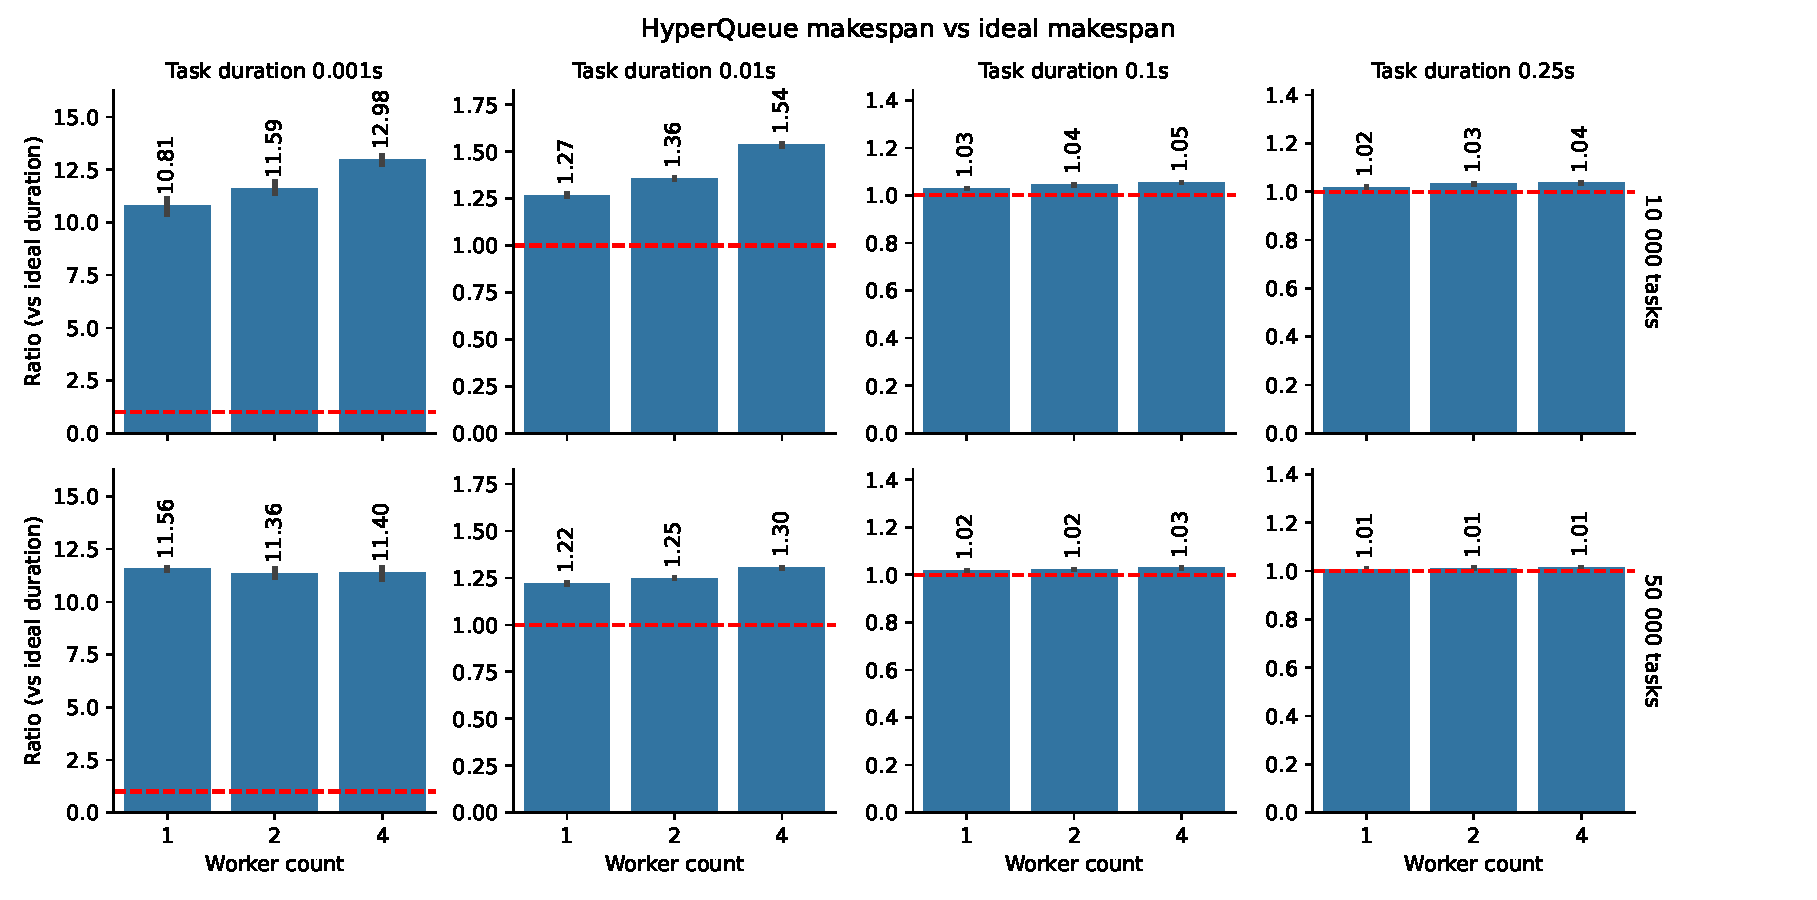
\includegraphics[width=\textwidth]{imgs/hq/charts/total-overhead-vs-ideal}
	\caption{Total overhead of \hyperqueue{} (ratio vs theoretically ideal makespan)}
	\label{fig:hq-overhead-vs-ideal}
\end{figure}

The results of this experiment can be observed in~\Autoref{fig:hq-overhead-vs-ideal}. Each chart column shows
a different task duration; the rows separate different task counts. Within each chart, the
horizontal axis represents the number of used workers, while the vertical axis shows the duration
needed to execute the task graph in \hyperqueue{}, normalized to the theoretical ideal
duration. The ideal duration is marked with a red horizontal dotted line. For example, the value
$1.05$ specifies that the \hyperqueue{} execution was
$5\%$ slower than the theoretically ideal duration.

We can see that for tasks that last for \SI{100}{\milli\second} or more, the overhead of
\hyperqueue{} is within $5\%$ of the ideal makespan, and with the larger
task graph that contains $50$ thousand tasks, the overhead stays within
$3\%$. The overhead increases slightly with an added number of workers, which is
expected; the scheduler needs to perform more work and the server also communicates with more
workers over the network.

The situation becomes more interesting in the case where the task duration is only
\SI{1}{\milli\second}. Here the overhead of \hyperqueue{} seemingly becomes very large.
We have examined this situation in detail and found out that the issue is caused mostly by slow
command execution performance on Karolina. Our calculation of the theoretically ideal makespan
assumes that the executed command will last for exactly \SI{1}{\milli\second}, but from our
experiments, even running a completely empty process on Karolina takes \emph{at least}
\SI{500}{\micro\second}, and executing a program that is supposed to sleep for
\SI{1}{\milli\second} can take several milliseconds. Because the overhead of actually executing
the command is so large, it skews the total overhead of \hyperqueue{}, as it is not able
to reach that theoretically ideal makespan, since the execution of commands takes more time than
expected. Note that this would be an issue for any task runtime that executes a command in each
task, and there is not that much that \hyperqueue{} could do to avoid this overhead.

\begin{figure}[h]
	\centering
	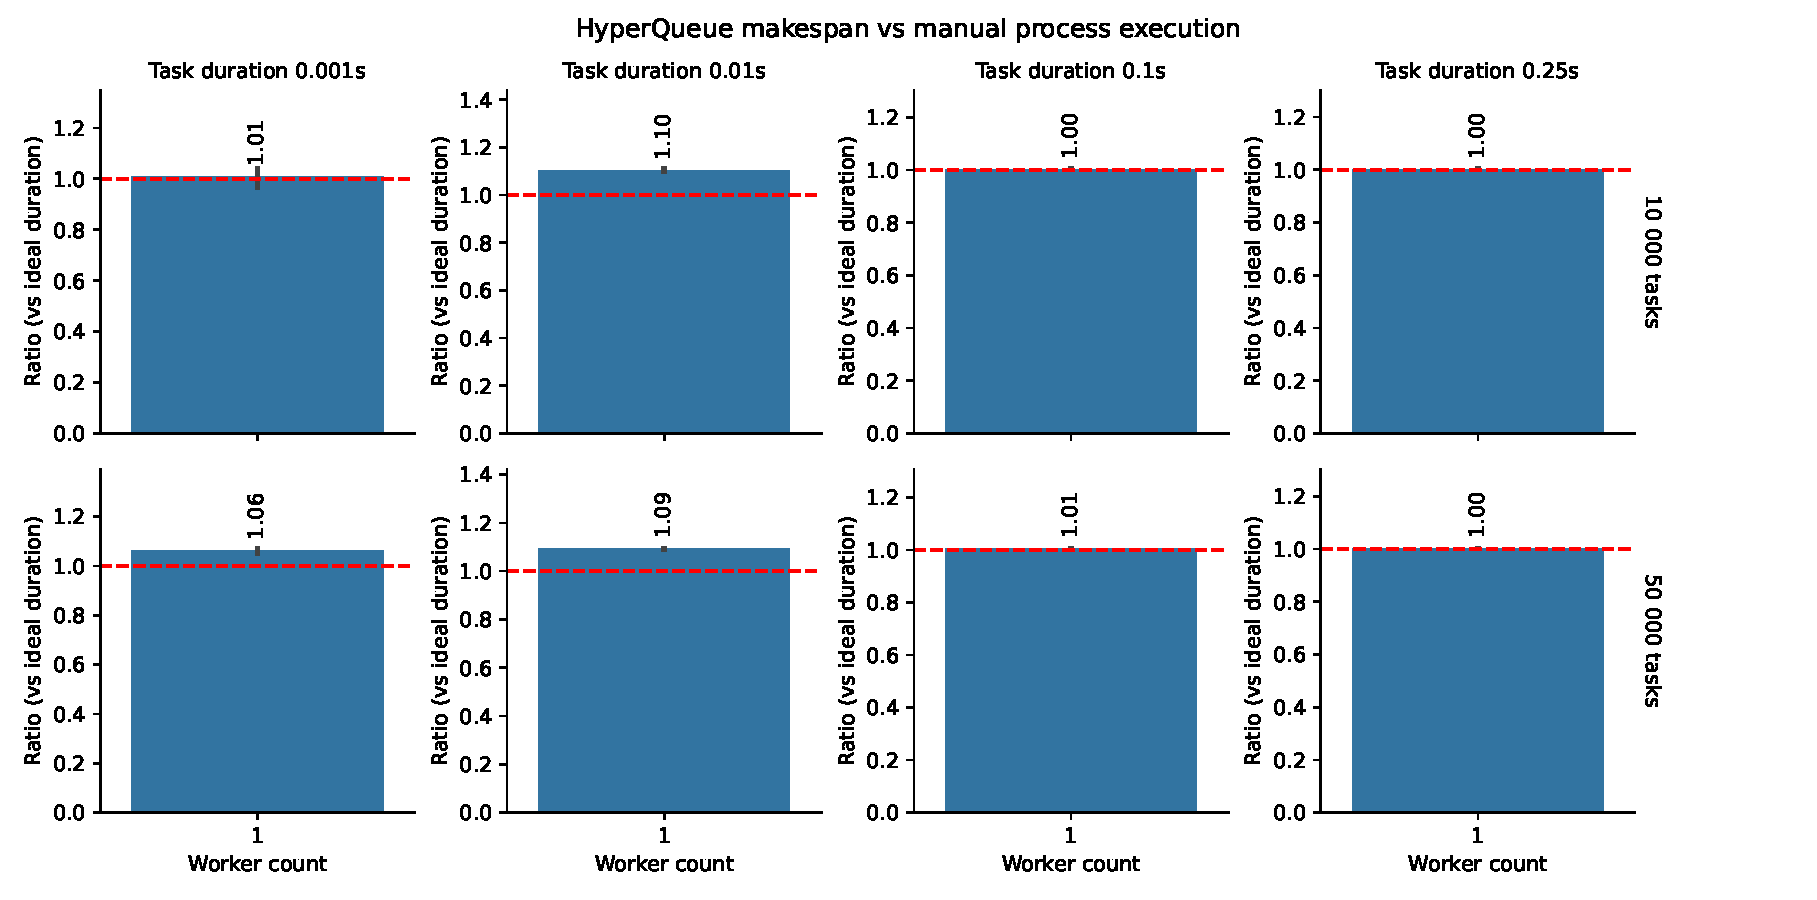
\includegraphics[width=\textwidth]{imgs/hq/charts/total-overhead-vs-manual}
	\caption{Total overhead of \hyperqueue{} (ratio vs manual process execution)}
	\label{fig:hq-overhead-vs-manual}
\end{figure}

To provide a fairer evaluation of the overhead of \hyperqueue{} for short tasks, we have
also evaluated it against a different baseline, which is not based on a theoretical calculation,
but on the actual performance of command execution on Karolina. We have implemented a simple
program that executes the same tasks (\texttt{sleep} processes) as
\hyperqueue{}, in parallel on all $128$ available cores. This provides a
more reasonable baseline that takes into account the overhead of command execution on Karolina. The
results of this experiments can be seen in~\Autoref{fig:hq-overhead-vs-manual}. The baseline is marked with a
horizontal red line; it represents the fastest measured time to execute the given number of
processes. We have performed this experiment only with a single worker, because our baseline
program did not implement multi-node distribution. Based on these results, we can see that for the
\emph{simple workflow}, the actual overhead of \hyperqueue{} (when compared to manually
running the commands without a task runtime) stays within
$10\%$.

\subsection{Task throughput}
\label{sec:hq-exp-task-throughput}
The previous experiment has evaluated the total overhead of \hyperqueue{} while taking
into account the time to execute tasks. To further examine the inner overhead of scheduling and
network communication, in this experiment we evaluate the possible task throughput (number of tasks
processed per second) using the \emph{zero worker} mode. In this mode, \hq{}
performs all operations that it does normally (managing tasks and workers, scheduling, sending
network packets), but it does not actually execute the tasks; the corresponding worker immediately
marks each task as completed instead. This allows us to examine the overhead of
\hyperqueue{} without it being affected by process spawning, which can have severe
overhead, as was demonstrated in the previous experiment. We have benchmarked the
\emph{simple workflow} containing from $10$ thousand to $1$
million tasks, with varying worker counts (up to $16$ workers and thus
$2048$ \gls{cpu} cores).

\begin{figure}[h]
	\centering
	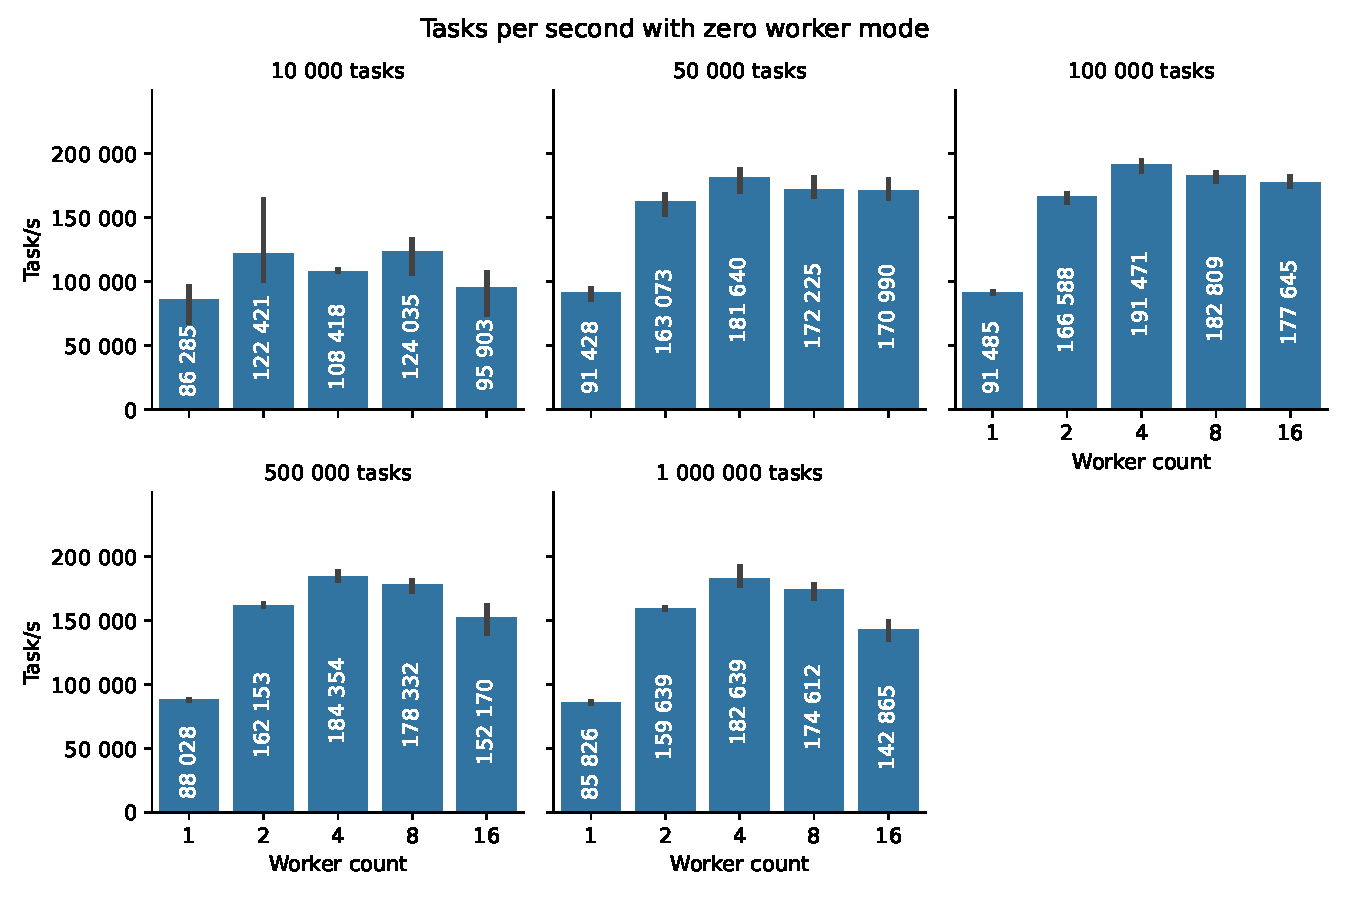
\includegraphics[width=0.8\textwidth]{imgs/hq/charts/task-per-s}
	\caption{Tasks processed per second with \emph{zero worker} mode}
	\label{fig:hq-tasks-per-s}
\end{figure}

The results can be observed in~\Autoref{fig:hq-tasks-per-s}. The horizontal axis displays the number of
tasks in the task graph, while the vertical axis displays the achieved throughput measured in tasks
processed per second. In theory, the throughput should be increasing with more added workers. For
the smallest task graph with $10$ thousand tasks, the throughput increases up to
four workers ($512$ cores), then it decreases; the task graph is too small and the
constant overhead factors start dominating over the available parallelism. For task graphs with up
to $100$ thousand tasks, the throughput increases up to four workers, where it
saturates. For even larger task graphs, the throughput once again starts decreasing with more than
four workers; the overhead of network communication and scheduling starts to dominate.

The absolute numbers of the achieved throughput demonstrate that \hyperqueue{} has very
little baseline overhead, and can in theory execute hundreds of thousands of tasks per second. The
tasks would have to be shorter than approximately \SI{5}{\micro\second} to fully saturate the
throughput achievable by \hyperqueue{}. Such a task duration is uncommon for scientific
workflows (indeed, on Karolina even starting a new process takes a hundred times longer); it is
more common for task-parallel programming models that have been described
in~\Autoref{sec:task-granularity}, which are operating on a very different level of granularity than what
\hyperqueue{} was designed for. This task throughput is orders of magnitude higher than
throughput measured for the \parsl{}, \fireworks{} and
\dask{} task runtimes, as reported in~\cite{parsl}.

\subsection{Strong scaling}
\label{sec:hq-exp-scalability}
This experiment evaluates the ability of \hyperqueue{} to scale to many computational
resources, by executing the same task graph with increasing worker counts (up to
$64$ workers and thus $8192$ cores in total). Note that each
benchmark configuration in this experiment was measured only once because of the large amount of
computational resources required to execute tens of worker nodes.

We have designed two separate scenarios for this experiment. In the first one, we have selected a
fixed target makespan, so that the \emph{simple workflow} would be executed in approximately\
$5$ minutes ($300$ seconds) on a single worker, and benchmarked
three task graphs with increasing task counts, to examine how the scalability of
\hyperqueue{} changes based on the number of tasks in the task graph when the total
computational workload stays the same. The task duration of each task was scaled accordingly for
each graph, so that the total makespan on a single worker would be $5$ minutes.
The benchmarked worker counts were $1$, $2$,
$4$, $8$, $16$, $32$ and
$64$.

\begin{figure}[h]
	\centering
	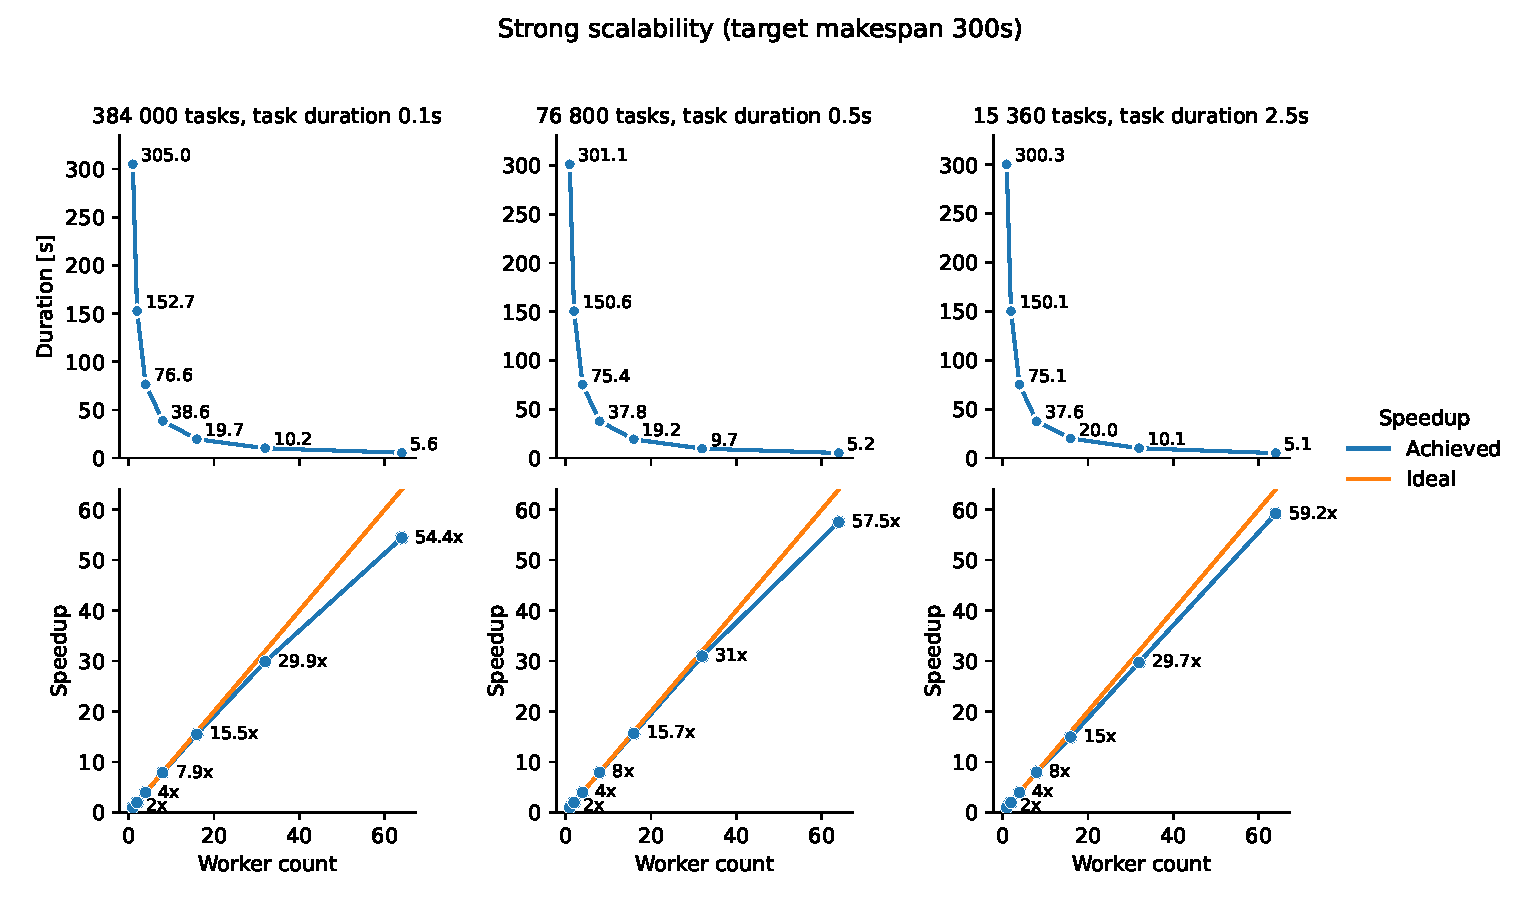
\includegraphics[width=\textwidth]{imgs/hq/charts/scalability-fixed-makespan}
	\caption{Strong scalability of \hyperqueue{} with a fixed target makespan
	(\SI{300}{\second})}
	\label{fig:hq-scalability-fixed-makespan}
\end{figure}

The results of the benchmark with a fixed makespan can be observed in~\Autoref{fig:hq-scalability-fixed-makespan}. The
horizontal axis displays the number of workers used for executing the task graph. In the top row,
the vertical axis shows the measured makespan; in the bottom row, the vertical axis shows speedup
against the measured makespan on a single worker. We can see that for all three measured task
durations, \hyperqueue{} was able to scale reasonably up to $64$
workers, and it was able to compute the whole task graph in approximately $5$
seconds. In the best case, with tasks that took \SI{2.5}{\second} to execute, it provided a
$59.2$x speedup with $64$ workers. In the worst case, with tasks
that lasted \SI{100}{\milli\second}, it provided a $54.4$x speedup with
$64$ workers. With task duration \SI{0.1}{\second} and
$64$ workers, \hyperqueue{} was able to dispatch almost
$70$ thousand tasks per second.

In the second scenario, we fixed the task duration of each task to $1$ second,
and then varied the task count. This allowed us to examine how the scalability of
\hyperqueue{} changes with an increasing workload.

\begin{figure}[h]
	\centering
	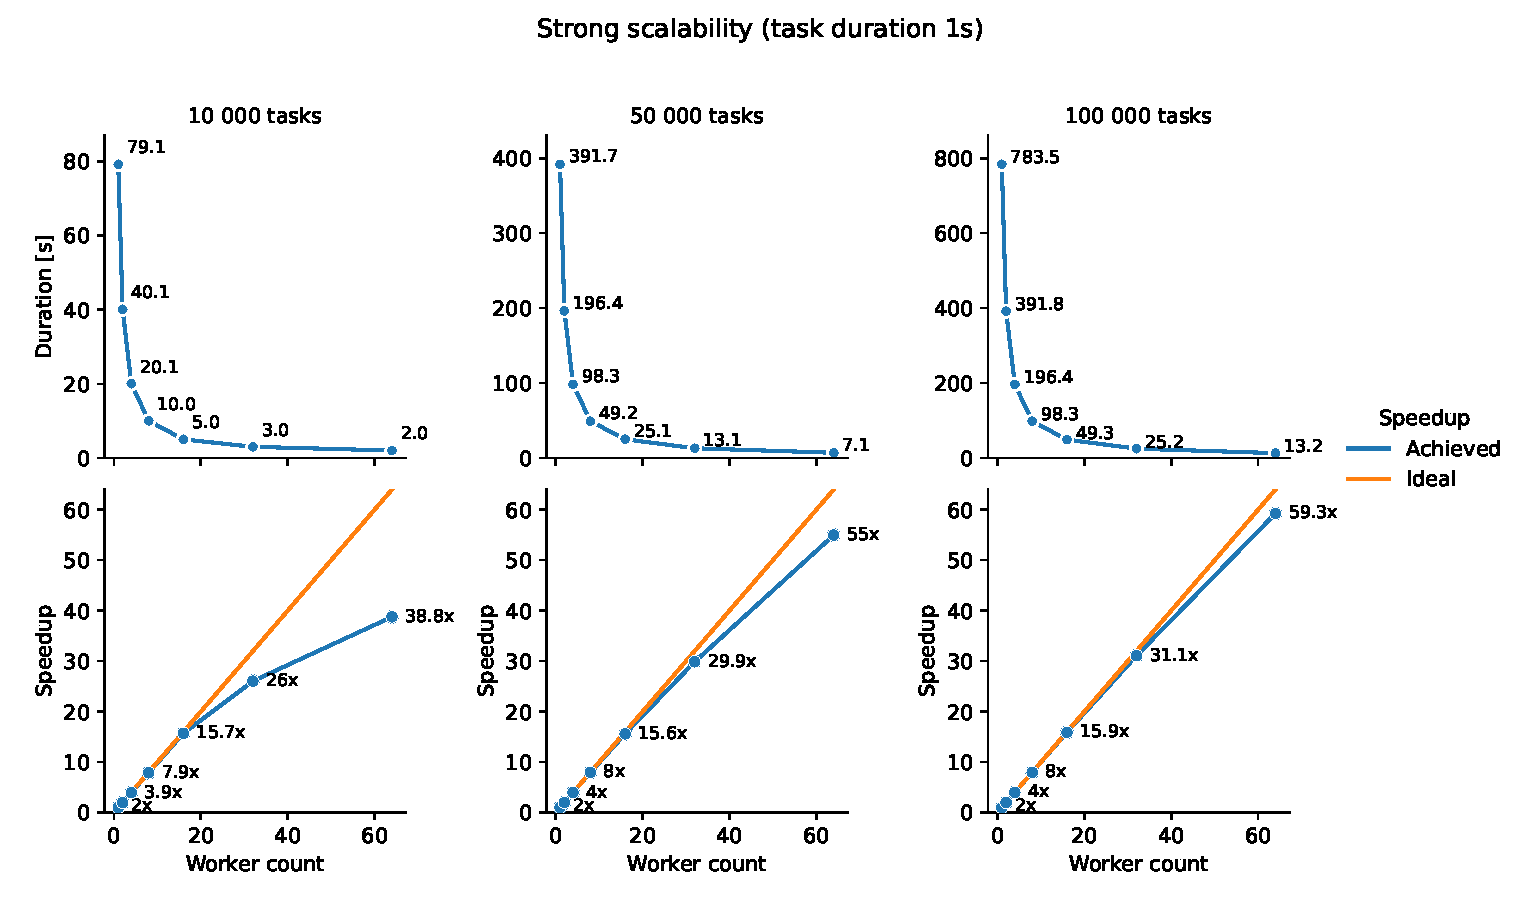
\includegraphics[width=\textwidth]{imgs/hq/charts/scalability-fixed-task-duration}
	\caption{Strong scalability of \hyperqueue{} with a fixed task duration (\SI{1}{\second})}
	\label{fig:hq-scalability-fixed-task-duration}
\end{figure}

We can observe the results in~\Autoref{fig:hq-scalability-fixed-task-duration}. We can see that the scalability improves
with the number of tasks; with $100$ thousand tasks, \hyperqueue{} is
able to provide a $59$x speedup with $64$ workers. On the other
hand, with only $10000$ tasks, the speedup in this case reaches only
$38.8$x, because there are not enough tasks to saturate all workers. With
$64$ workers that each have $128$ cores, the total number of
cores managed by \hq{} is $8192$. Therefore, in this small task
graph, each worker barely gets a single task to compute.

In general, the results indicate that \hyperqueue{} introduces very little overhead, and
is able to scale to a large amount of computational resources (tens of nodes and thousands of
cores) and also to large amounts of tasks (hundreds of thousands) without an issue.

\subsection{Performance comparison of \dask{} and \hq{}}
\label{sec:hq-exp-dask}
This experiment evaluates basic performance differences between the \dask{} task
runtime and \hyperqueue{}. We have evaluated \emph{dask/distributed}
$2024.7.0$ running under CPython $3.10.8$, with a disabled monitoring
dashboard for improved performance. All measurements in this experiment were performed only once,
to reduce the required computational resources.

We have evaluated the scalability of both runtimes on the \emph{simple workflow} with a target
makespan set to \SI{30}{\second} on a single worker, with an increasing number of workers
and a varying number of tasks. In this scenario, \dask{} was benchmarked in three
separate worker configurations, with $1$ process per node and
$128$ threads per process ($1p/128t$), with $8$
processes per node and $16$ threads per process ($8p/16t$) and
with $128$ processes per node and $1$ thread per process
($128p/1t$). The reason for choosing different process/thread combinations has been
extensively explained in~\Autoref{dask:evaluation}; we chose two extremes ($1$
process and $128$ processes) and then a compromise with $8$
processes per node, according to recommendations in the \dask{}
documentation~\cite{dask-thread-recommendation}.

\begin{figure}[h]
	\centering
	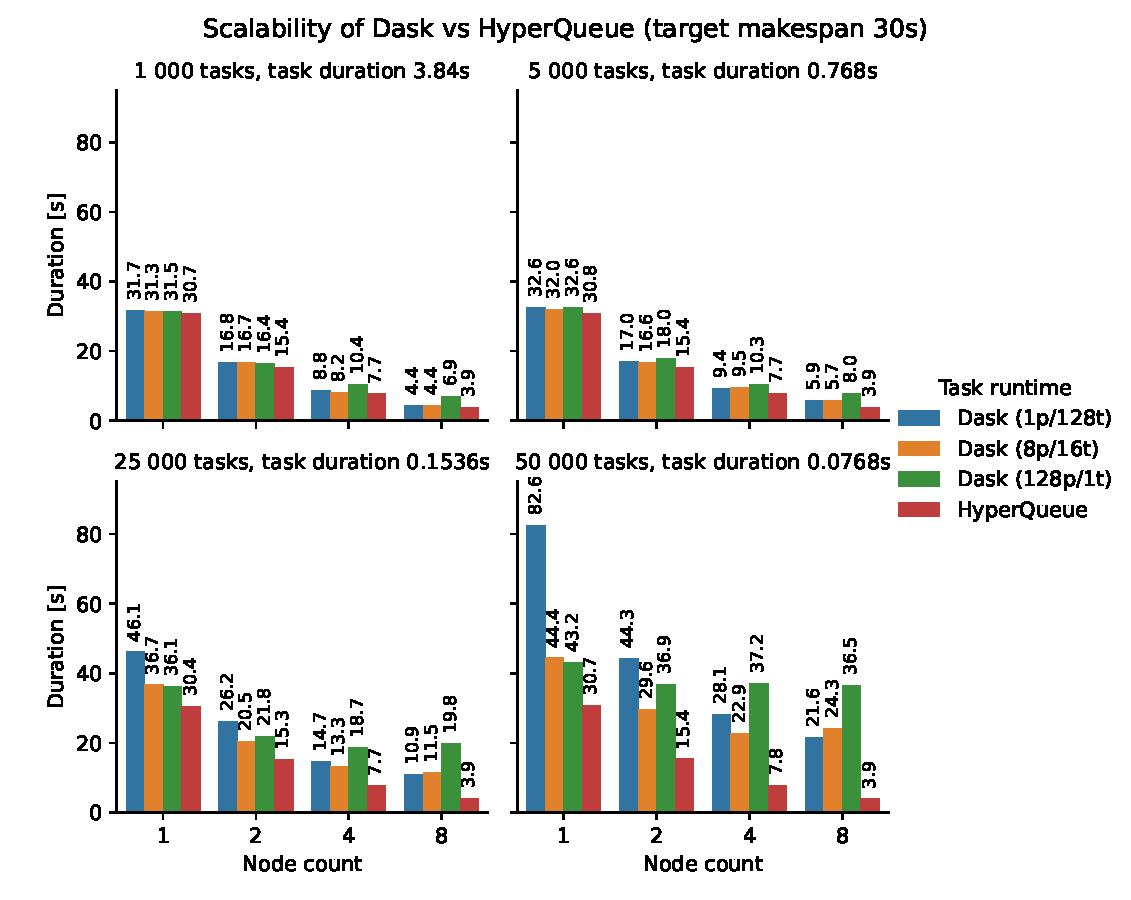
\includegraphics[width=0.8\textwidth]{imgs/hq/charts/dask-vs-hq-sleep}
	\caption{Scalability of \hyperqueue{} vs \dask{} with a fixed target makespan
	(\SI{30}{\second})}
	\label{fig:hq-dask-sleep}
\end{figure}

The results of this experiment are displayed in~\Autoref{fig:hq-dask-sleep}. The individual charts
display separate task graphs with varying task counts (in each case, the task graph should have a
makespan of $30$ seconds on a single node). The horizontal axis shows the amount
of used nodes and the vertical axis displays the makespan. Note that we are using the term
\emph{node count} instead of \emph{worker count} here, because each
\dask{} process spawned per node is technically a separate worker. We can see that
the in the case of \dask{}, the performance depends a lot on the number of tasks in
the task graph, and also on the task duration. With only $1000$ tasks and task
duration in the range of seconds, \dask{} is able to scale relatively well in all
three configurations, although it is still slightly slower than \hyperqueue{}. However,
with a larger number of tasks (tens of thousands), and tasks that last only hundreds or tens of
milliseconds, the performance of \dask{} decreases very quickly.

We can also see differences between the three \dask{} configurations, particularly
in the benchmark with $50000$ tasks. With a single node, \dask{} is
unable to keep up with the number of tasks, and it has a twice longer makespan than when multiple
worker processes are used. On the other hand, once the number of nodes is increased, the situation
reverses, and the configuration with a single worker per node becomes the fastest one, because
\dask{} starts being overwhelmed by the number of connected workers. This suggests
that some amount of manual tuning based on the number of used nodes and workers might be required
to achieve optimal performance of \dask{} workflows. Conversely,
\hyperqueue{} was able to keep a consistent performance profile in this experiment,
without being affected by the number of tasks or the task duration. And since each
\hq{} worker always manages all resources of a single node, it does not require
any manual worker tuning.

Note that this benchmark actually presents a sort of a best-case scenario for
\dask{}. It executes its tasks as Python functions; therefore, it does not need to
start a new Linux process per task, unlike \hyperqueue{}. Furthermore, since each task
simply sleeps for a specified duration, it releases the \gls{gil} and therefore does
not block other Python threads of the worker, which can thus perform other work concurrently.

\begin{figure}[h]
	\centering
	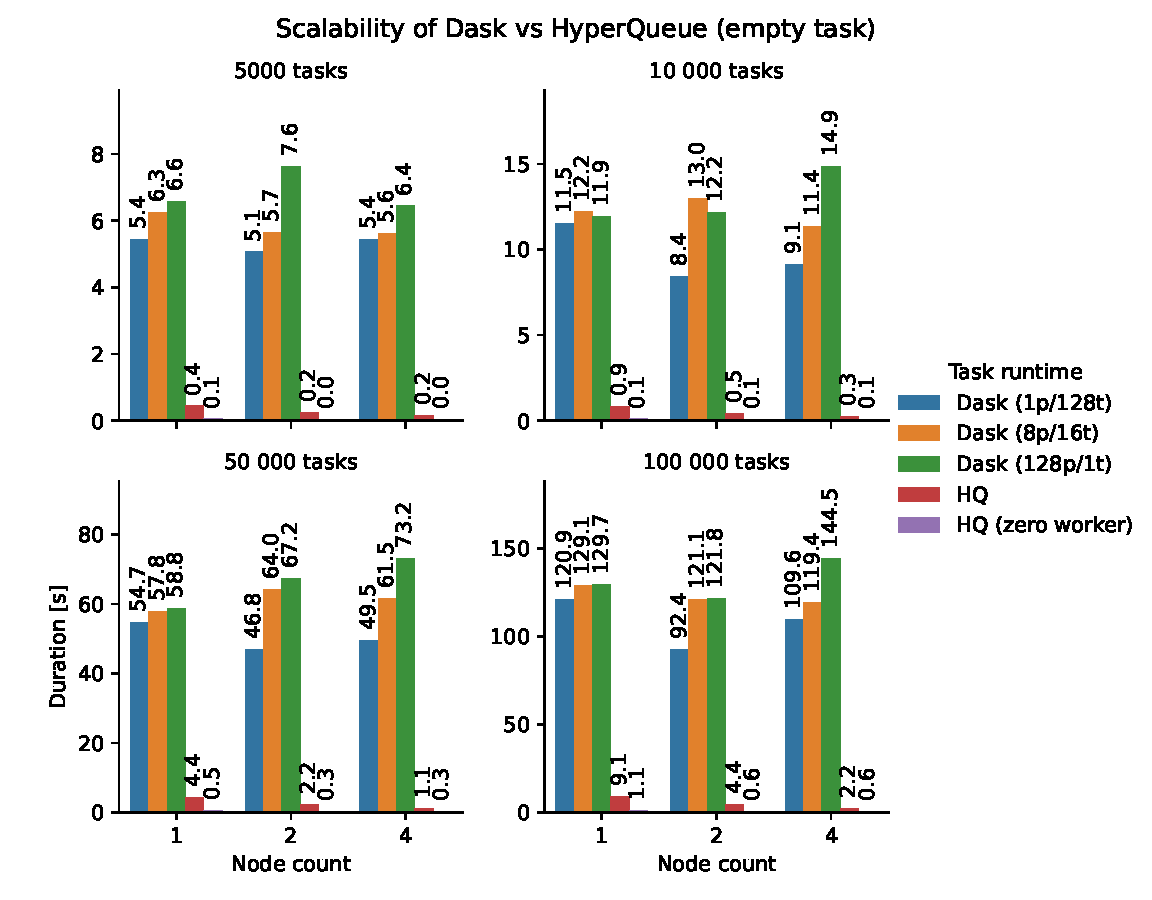
\includegraphics[width=0.8\textwidth]{imgs/hq/charts/dask-vs-hq-empty}
	\caption{Scalability of \hyperqueue{} vs \dask{} with an empty task}
	\label{fig:hq-dask-empty}
\end{figure}

We have further examined the baseline overhead of \dask{} by executing an empty
task (an empty Python function), which emulates the \emph{zero worker} mode of
\hyperqueue{}, as it shows how the task runtime scales with the fastest possible task
execution. We have compared this empty task execution with running the fastest possible task in
\hyperqueue{} (by spawning a process that immediately exits) and also with the \emph{zero worker} mode of \hyperqueue{}.

The results of this experiment can be seen in~\Autoref{fig:hq-dask-empty}. The horizontal axis shows
the node count, and the vertical axis displays the makespan. Here we can observe a large difference
between the inner overhead of \hyperqueue{} and \dask{}, which struggles
to keep up with large amounts of very short tasks. This is of course an artificial scenario because
the tasks are empty; however, it does demonstrate that \dask{}'s can have
performance issues with large or very granular task graphs. It is also clear that the overhead of
\dask{} increases quickly with multiple added workers, which is further exacerbated
when multiple workers per node are used.

\subsection{Resource variants}
\label{sec:hq-exp-resource-variants}
This experiment evaluates the load-balancing benefits of \emph{resource variants}. We simulate a
task graph with a computation that can run either on a \gls{gpu} or on a
\gls{cpu}. Assume that there is a limited number of accelerators on a node , but
there are also additional \gls{cpu} cores that can be used for the computation. The
simplest approach is to configure all tasks to run on the \gls{gpu}. However, this
means that the \gls{cpu} resources will be wasted. To avoid that, we can assign a
fixed portion of the tasks to run on the \gls{cpu}; however, deciding this up front
will not allow \hyperqueue{} to execute such tasks on a \gls{gpu} even if
one was available at the given moment. Using resource variants, we can state that a task should be
executed primarily on a \gls{gpu}, but if one is not currently available, then it can
also run on the \gls{cpu}.

In this experiment, we evaluate the simple workflow with $300$ tasks, on a node
with $8$ virtual \glspl{gpu} and same number of
\glspl{cpu}. To emulate the performance difference between the \gls{gpu}
and the \gls{cpu}, tasks executed on the accelerator will sleep for
\SI{1}{\second}, and tasks executed on the \gls{cpu} will sleep for a
multiple of this duration, according to a given ratio (which is a benchmark parameter).

\begin{figure}[h]
	\centering
	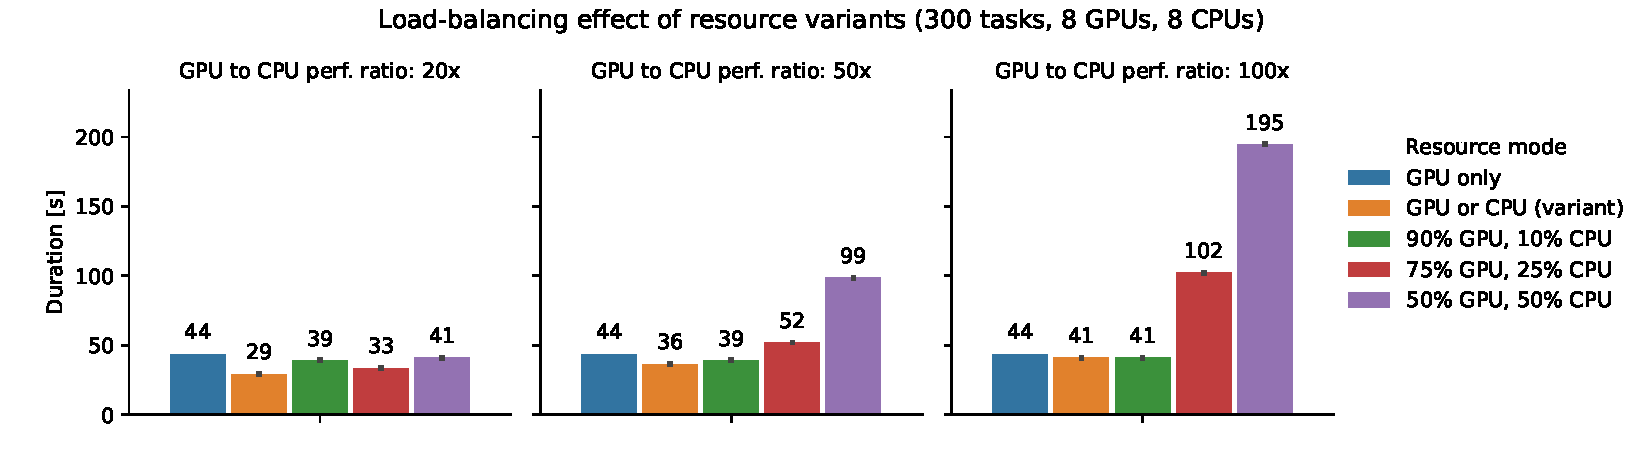
\includegraphics[width=\textwidth]{imgs/hq/charts/alternative-resources}
	\caption{Load-balancing effect of resource variants}
	\label{fig:hq-resource-variants}
\end{figure}

The results of the experiment can be observed in~\Autoref{fig:hq-resource-variants}. The vertical axis
displays the makespan; the five bars represent different configurations of resources. In the
\emph{\gls{gpu} only} mode, all tasks were configured to run on a single \gls{gpu}.
In the \emph{\gls{gpu} or \gls{cpu}} mode, tasks were configured to run either on the
\gls{gpu} or on the \gls{cpu}, using resource variants. The remaining
three modes assigned a specific fraction of tasks to run on the \gls{gpu}; the rest
was executed on the \gls{cpu}. The three charts show results for different values of
the \gls{gpu} vs \gls{cpu} performance ratio, i.e.\ how much faster was
the task running on a \gls{gpu}.

We can see that unless the \gls{gpu} ratio is too high or we assign too many tasks to
the \gls{cpu}, it is beneficial to also leverage the \gls{cpu}
resources, rather than using only \glspl{gpu}. With \gls{cpu} fractions
determined manually in advance, the result depends heavily on the \emph{\gls{gpu} ratio}, and in
certain configurations it can make the makespan significantly longer. This would thus be both less
efficient and more laborious to configure for the user. On the other hand, when the resources for
each task are configured using two resource variants (either \gls{gpu} or
\gls{cpu}), \hyperqueue{} is able to dynamically adapt to all three
\gls{gpu} ratios. In all three scenarios, the makespan with resource variants is
strictly smaller than with \glspl{gpu} only, and it either surpasses or matches the
best result achieved with a predetermined fraction of tasks running on the \gls{cpu}.
This shows that resource variants can help achieve better hardware utilization without requiring
the user to fine-tune resource configurations of individual tasks in the task graph.

\subsection{Worker \gls{cpu} utilization}
\label{sec:hq-cpu-utilization}
One of the primary metrics that task graph users care about is hardware utilization -- how well can
a task graph (executed with a given task runtime) make use of available resources? This experiment
examines the average \gls{cpu} utilization of worker nodes while executing a task
graph with \hyperqueue{}, both for tasks with a uniform duration and also for tasks with
a skewed distribution of durations. We have benchmarked the \emph{simple workflow} with
$10$ thousand tasks, where each task fully utilizes a full
\gls{cpu} core by executing the \texttt{stress} UNIX utility (instead of just
sleeping). This task graph was executed on $4$ workers, whose
\gls{cpu} utilization was periodically measured over the course of the computation.

\begin{figure}[h]
	\centering
	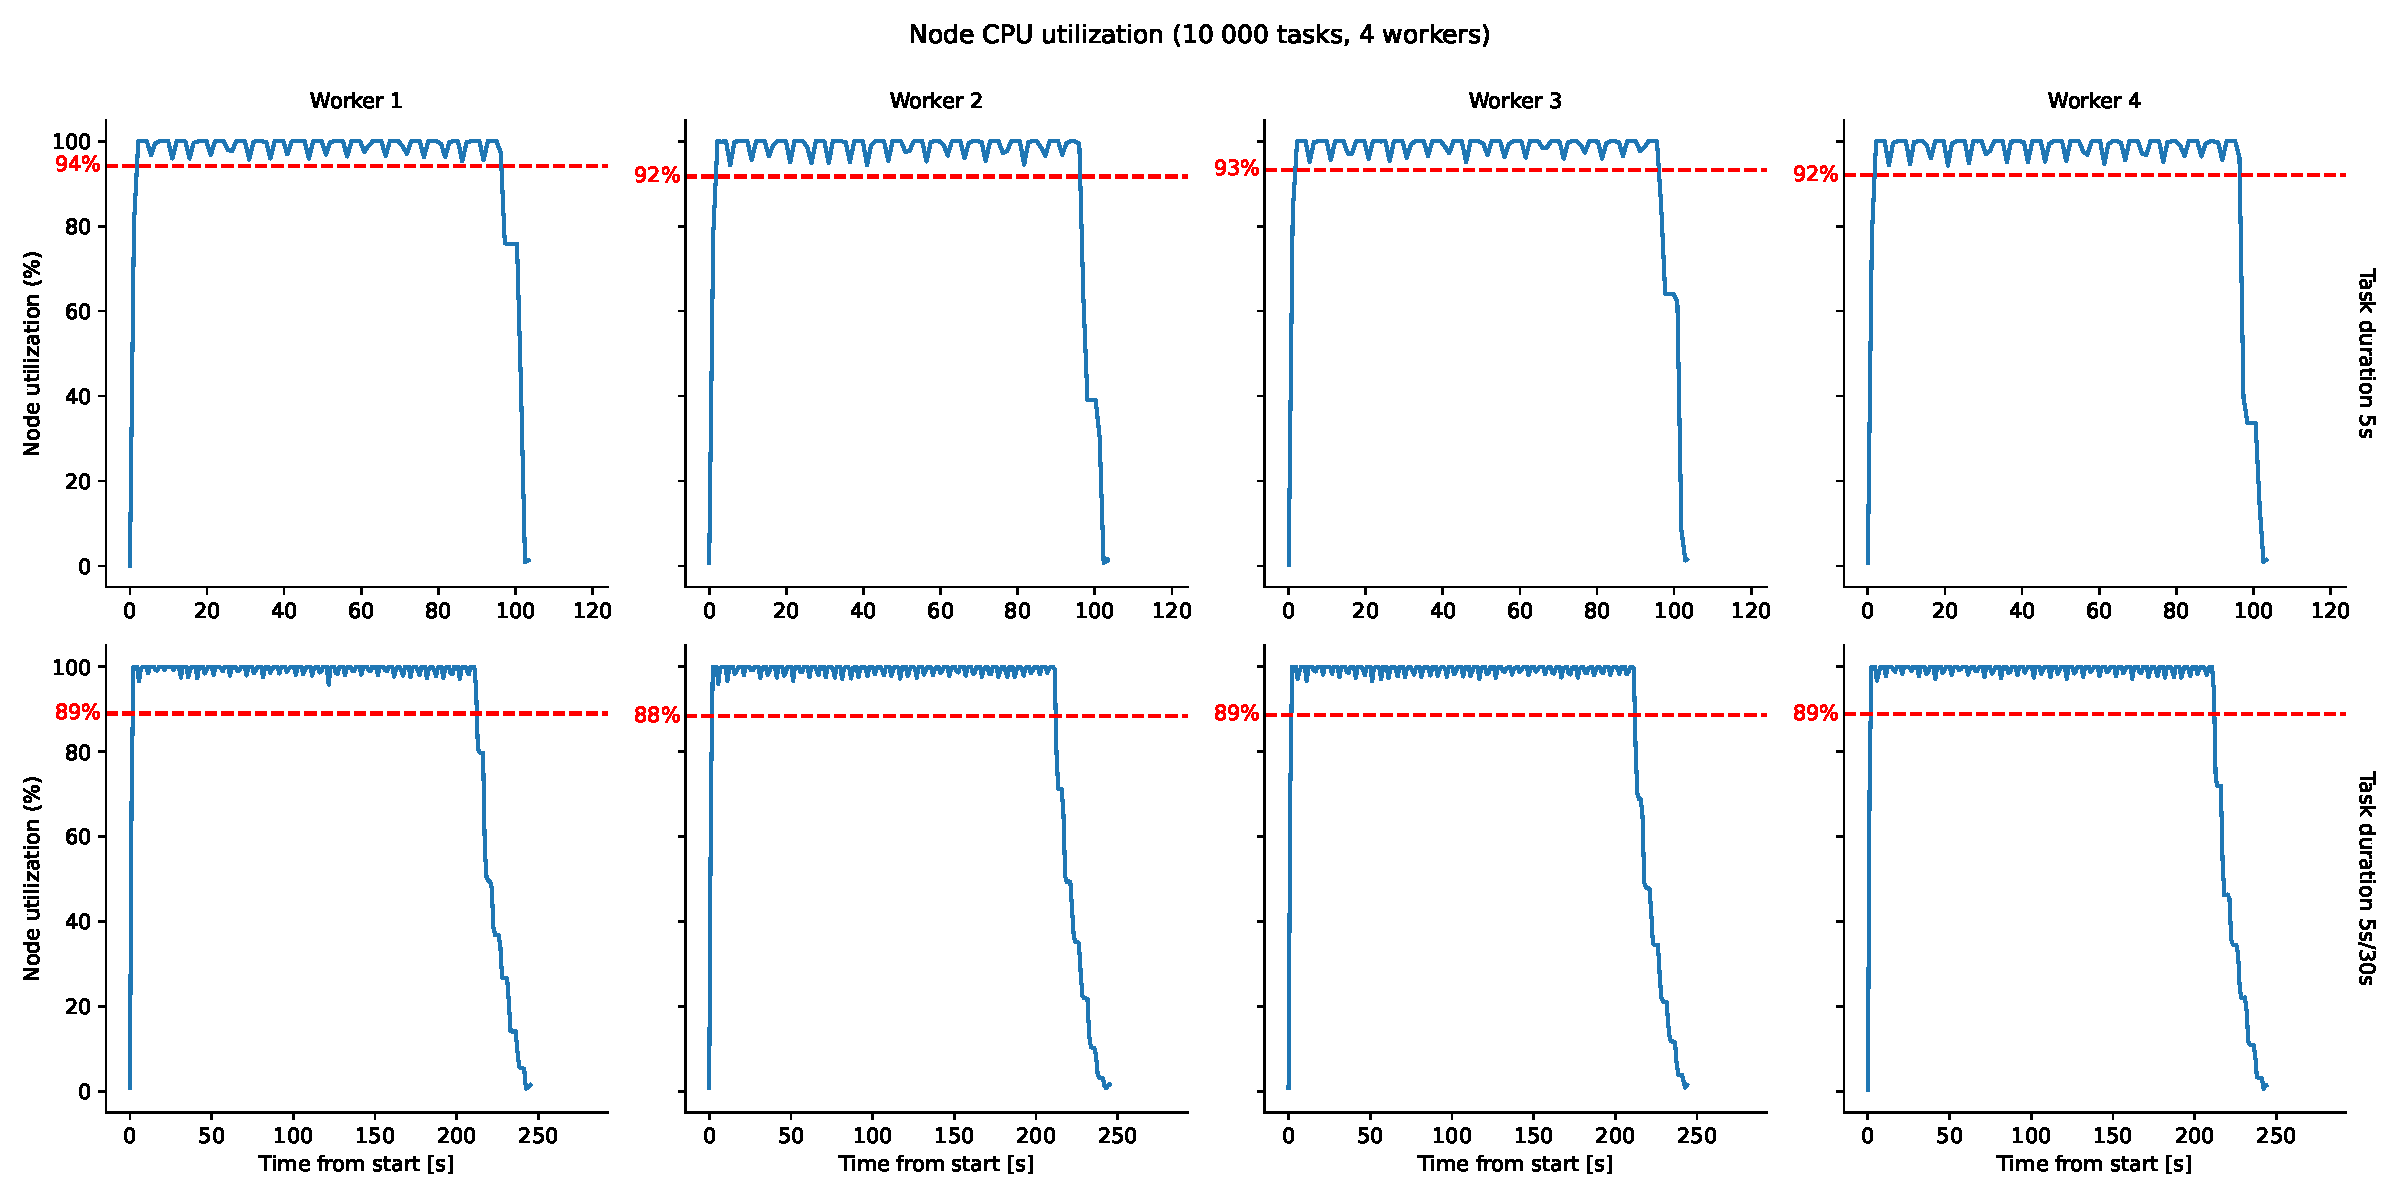
\includegraphics[width=\textwidth]{imgs/hq/charts/scalability-stress-utilization}

	In the bottom row, 75\% of tasks last \SI{5}{\second}, 25\% of tasks last
	\SI{30}{\second} \caption{\gls{cpu} utilization of \hyperqueue{} worker nodes} \label{fig:hq-cpu-utilization}
\end{figure}

The results are shown in~\Autoref{fig:hq-cpu-utilization}. The horizontal axis shows the progress of the
computation in seconds, the vertical axis displays the average \gls{cpu} utilization
over all $128$ cores for each separate worker. The red horizontal line marks the
total average utilization of each worker over the course of the whole computation. The top row
displays a situation where all tasks in the task graph have a uniform duration of
$5$ seconds. In this case, \hyperqueue{} workers keep their average
utilization above $90\%$. Note that it takes some amount of time for each
\texttt{stress} invocation to fully reach full core utilization, and since all tasks have
the same duration, the tasks perform this ramp-up process in a mostly synchronized fashion. This
causes the ``teeth'' in the utilization chart. Therefore, it is not realistic to reach full
$100\%$ node utilization with this task graph.

The second row displays a situation where the workload is skewed. Most ($75\%$) of
the tasks still have a duration of \SI{5}{\second}; the remainder simulates a ``long tail''
of slower tasks that take \SI{30}{\second} to execute. This is a more difficult situation
for achieving high utilization; because some tasks are longer, they might get stuck executing at a
time when other resources can no longer be utilized. We can observe this towards the end of the
workflow execution, where approximately $30$ seconds before the end, the
utilization starts to drop. However, even for this skewed task graph, the average
\gls{cpu} utilization was kept at almost $90\%$.

\subsection{Server \gls{cpu} consumption}
\label{sec:hq-exp-server-cpu-consumption}
The \hyperqueue{} server component is primarily designed to be executed on login nodes
when deployed on supercomputers. This could pose a problem if it consumed too many system
resources, because login nodes are shared by multiple users, and they are not designed for
computationally intensive tasks. Some clusters even forcefully limit the total amount of
\gls{cpu} time that can be consumed by processes running on login
nodes~\cite{leonardo_time_limit}, and terminate the process if it exceeds the maximum allowed time.

To evaluate how many resources the server consumes, we have performed an experiment where the
server had to schedule a large number of tasks in a short time period (which acts as a sort of a
stress test), and we measured its total \gls{cpu} time consumption across all cores.
The server was running on a login node, and it was managing up to $12$ workers
($1536$ cores) and up to $200$ thousand tasks. Each worker was
deployed on a computational node, so that the server had to communicate with the workers over the
network. The benchmark was executed with a fixed makespan; the duration of each task was scaled so
that the whole task graph would finish computing in one minute. We measured the total amount of
\gls{cpu} time consumed by the server (both in user-space and in the kernel), using
standard Linux process monitoring tools.

\begin{figure}[h]
	\centering
	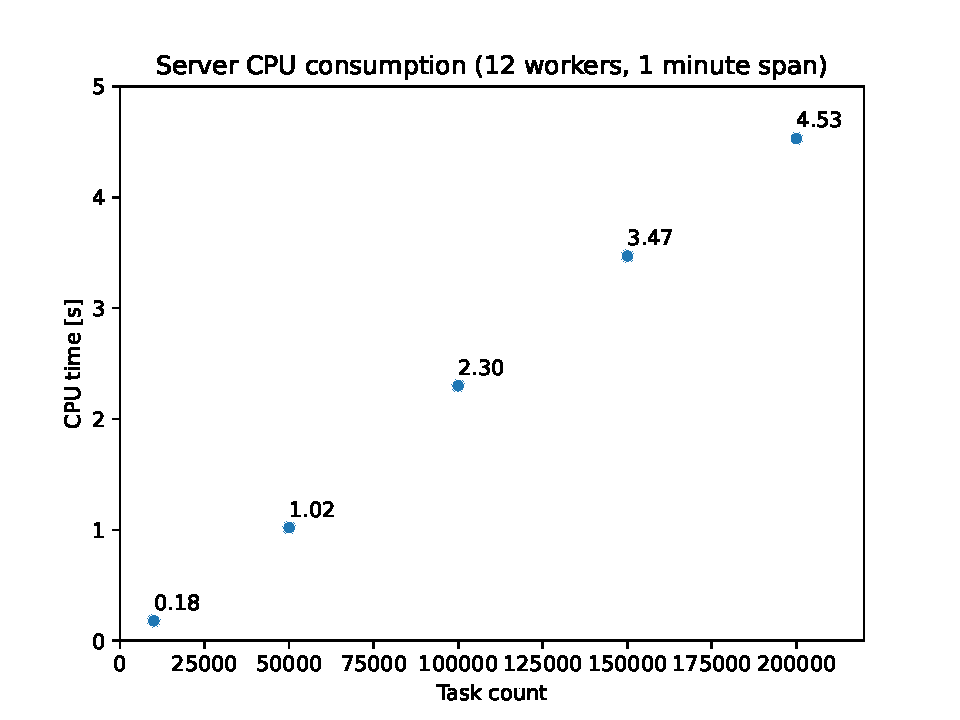
\includegraphics[width=0.6\textwidth]{imgs/hq/charts/server-utilization-tasks}
	\caption{\gls{cpu} time consumption of the \hyperqueue{} server with an increasing
	number of tasks}
	\label{fig:hq-server-cpu-consumption-tasks}
\end{figure}

\Autoref{fig:hq-server-cpu-consumption-tasks} shows how does the \gls{cpu} utilization of the
server change with a fixed number of workers ($12$) and an increasing number of
tasks. In this case, the server had to schedule the \emph{simple workflow} with number of tasks
ranging from $10$ to $200$ thousand. The horizontal axis shows
the number of tasks that were used for the given benchmark run, and the vertical axis shows the
\gls{cpu} time consumed by the server over the one-minute period. We can see that the
amount of \gls{cpu} resources scales approximately linearly with the number of tasks
scheduled by the server. In the worst case, the server has consumed less than five seconds of
\gls{cpu} time over one minute of real time, even though it had to schedule
$200$ thousand tasks within this short period, which is an extreme stress test
that far exceeds the rate of scheduled tasks in most scientific workflows. Over all the benchmarked
task counts, the average \gls{cpu} consumption of the server per second and per
$1000$ tasks was approximately \SI{0.0003}{\second}. In other words, for every
thousand tasks in the task graph, the server consumed approximately \SI{0.3}{\milli\second}
\gls{cpu} time every second.

\begin{figure}[h]
	\centering
	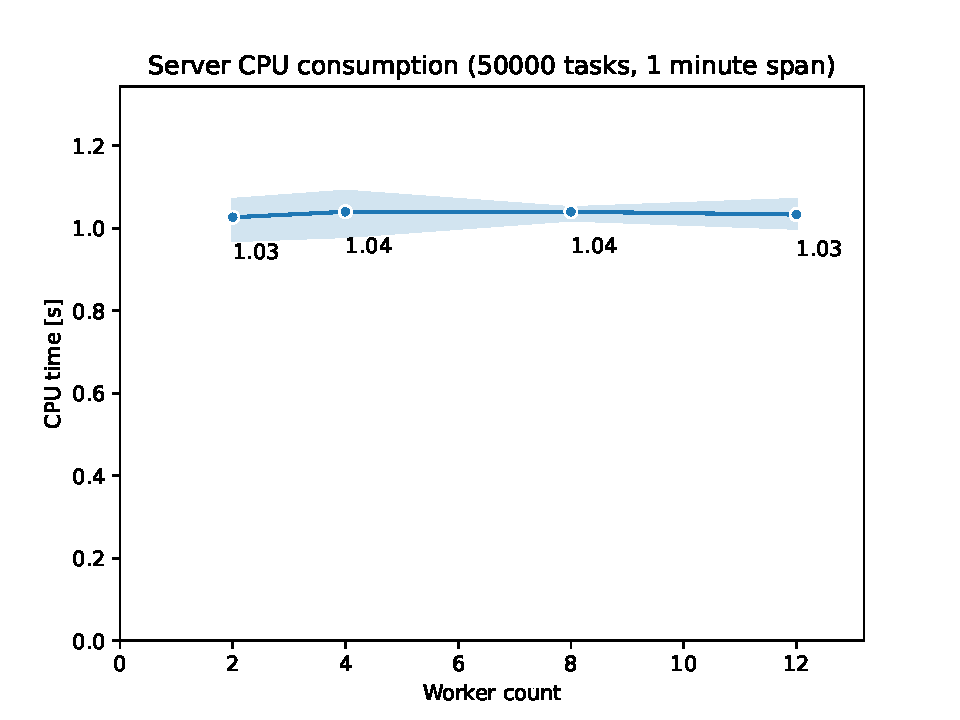
\includegraphics[width=0.6\textwidth]{imgs/hq/charts/server-utilization-workers}
	\caption{\gls{cpu} time consumption of the \hyperqueue{} server with an increasing
	number of workers}
	\label{fig:hq-server-cpu-consumption-workers}
\end{figure}

\Autoref{fig:hq-server-cpu-consumption-workers} displays a situation where the number of tasks
is fixed ($50000$), but the number of workers increases from
$2$ to $12$. The horizontal axis shows the number of workers
that were used for the given benchmark run, and the vertical axis shows the \gls{cpu}
time consumed by the server over the one-minute period. In this case, the consumption of the server
does not increase by a large amount with more added workers.

In terms of memory consumption, in the largest evaluated case with a task graph containing
$200$k tasks, the memory consumption of the server (measured through
\gls{rss}) was approximately \SI{120}{\mebi\byte}, which shows that the server
also does not consume large amounts of memory.

The amount of used resources will of course vary based on the executed workflow. However, this
experiment shows that the server consumes very few resources in general, and that it still has a
lot of leeway available even if some task graphs proved to be more computationally demanding than
the benchmarked stress test.

\subsection{Encryption overhead}
\label{sec:hq-exp-encryption-overhead}
As has already been noted in~\Autoref{hq:architecture}, \hyperqueue{} encrypts all network
communication between the server, the workers and the client. This encryption is performed because
the server is typically deployed on a login node, and thus the communication it performs can be in
theory observed by other users of the cluster. In this experiment, we have evaluated the overhead
of the encryption, by benchmarking \hyperqueue{} both with encryption enabled and
disabled.

We have benchmarked three instances of the \emph{simple workflow} containing
$10$, $50$ and $100$ thousand tasks
executed with $4$ \hyperqueue{} workers in two configurations; with
and without the \emph{zero worker} mode. Because the \emph{zero worker} mode does not
actually execute any tasks, it emphasizes the inner overhead of \hyperqueue{}, and should
thus also amplify potential differences in communication overhead caused by the encryption.

\begin{figure}[h]
	\centering
	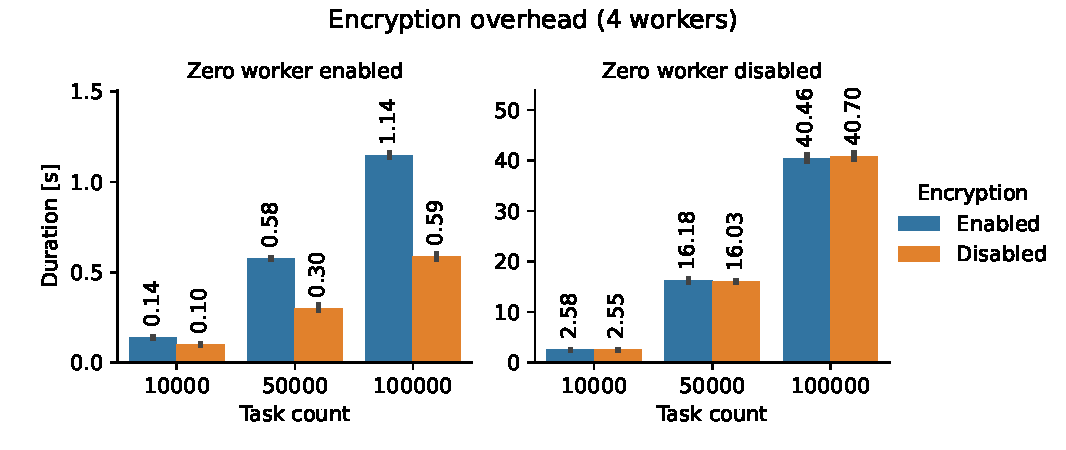
\includegraphics[width=0.8\textwidth]{imgs/hq/charts/encryption-overhead}
	\caption{Overhead of encryption in \hyperqueue{} communication}
	\label{fig:hq-encryption-overhead}
\end{figure}

We can observe the results of the experiment in~\Autoref{fig:hq-encryption-overhead}. The horizontal axis shows
the number of tasks in the benchmarked task graph, and the vertical axis shows the
\emph{makespan}. In the \emph{zero worker} mode (displayed on the left), it is clear
that encrypting the communication in fact produces a measurable overhead. In the largest measured
case with $100$ thousand tasks, the makespan is approximately twice longer with
encryption enabled. However, as soon as the tasks do any actual work (albeit it being the simplest
work possible), the encryption overhead is no longer noticeable and it does not affect the total
makespan of the task graph.

In more realistic workflows, the executed tasks will be almost certainly longer than just executing
the trivial~\texttt{sleep} command. In that case, the overhead of encryption will be even
less noticeable; the larger the duration of the executed tasks, the less important is the overhead
introduced by \hyperqueue{}. If some users would still not want to use encryption for
some reason, \hyperqueue{} could be easily modified to add the option to disable
encryption at runtime.

\subsection{Output streaming}
\label{sec:hq-exp-output-streaming}
In this experiment we evaluate the effect of the \emph{output streaming} mode, which can be used to
stream the outputs of \emph{stdout} and \emph{stderr} streams from individual
tasks to the \hyperqueue{} server, to avoid creating a large number of files on the
filesystem. We have benchmarked two task graphs without dependencies, with $10$
and $50$ thousand tasks, where each task generates a a fixed amount of data
($10$ and \SI{100}{\kibi\byte} per task). Each task simply outputs the
corresponding amount of data to its standard output (\emph{stdout}). The standard error
output is disabled and no output is printed to it. In the largest configuration, the task graph
produces approximately \SI{5}{\gibi\byte} of data in total.

With output streaming enabled, each task output is streamed to the server, which stores all data
sequentially into a single log file. Without output streaming, each task simply creates a single
file on disk and writes its \emph{stdout} output to it. The experiment was performed on
two different filesystem partitions of the Karolina cluster. The first partition, called SCRATCH,
uses the Lustre networked filesystem, which is designed for parallel high intensity
\gls{io} workloads~\cite{karolina_scratch}. It is a representative of a
high-performance filesystem, which can in theory reach up to \SI{700}{\gibi\byte}/s write
throughput. The second partition, called PROJECT, uses \gls{gpfs}, which is a much
slower filesystem implementation that focuses on providing high availability and
redundancy~\cite{karolina_project}.

\begin{figure}[h]
	\centering
	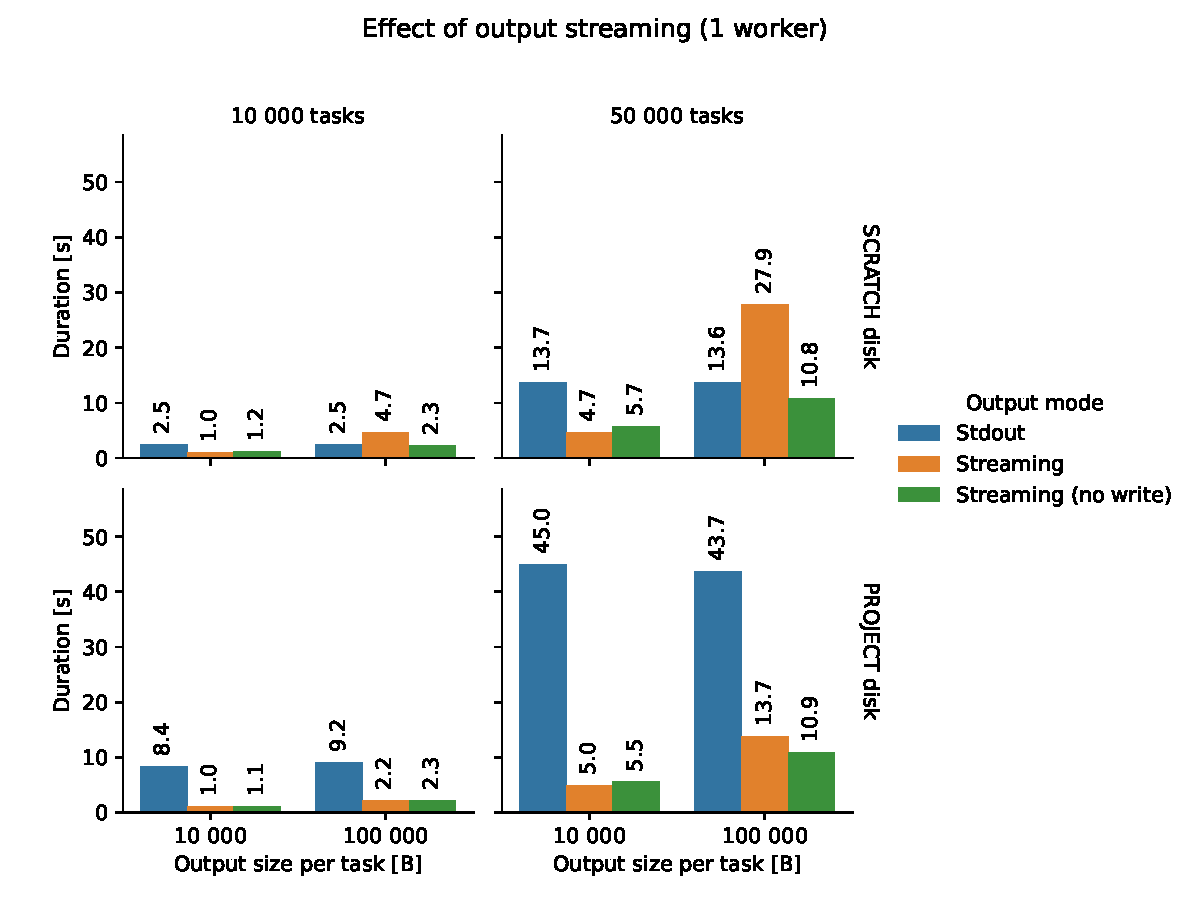
\includegraphics[width=0.7\textwidth]{imgs/hq/charts/io-streaming}
	\caption{Effect of output streaming on the makespan of tasks}
	\label{fig:hq-io-streaming}
\end{figure}

We can see the results of the experiment in~\Autoref{fig:hq-io-streaming}. The horizontal axis displays
the amount of output produced by each task and the vertical axis shows the makespan of the executed
task graph. The top row contains data for the SCRATCH filesystem; the bottom row contains data for
the PROJECT filesystem. Three separate configurations are displayed in the chart. In the
\emph{Stdout} mode, the task graph was executed without output streaming, while in the
\emph{Streaming} mode, the task graph was executed with output streaming. The third mode
will be described later below.

The results differ significantly based on the amount of output produced by each task, and also
based on the used filesystem. On the SCRATCH Filesystem, output streaming is able to reduce the
makespan approximately by half, in the case where each task outputs \SI{10}{\kibi\byte} of
data. However, when task output is larger (\SI{100}{\kibi\byte}), the situation reverses, and
output streaming becomes slower. This is caused by the fact that the sequential writing into the
log file by the server becomes a bottleneck, as it cannot be easily parallelized by the filesystem
(unlike e.g.\ writing to many files in parallel). We have confirmed this by benchmarking a third
mode, which we call \emph{Streaming (no write)}. In this configuration, output streaming was enabled;
therefore, the output of tasks was streamed over the network from workers to the server, but then
the server simply discarded the data and did not write it to the sequential log file. We can see
that without actually sequentially writing the data to the log file, the makespan is still shorter
than without output streaming. It is thus clear that the primary bottleneck in this case is in fact
the final write to the log file.

It should be noted that even though output streaming is slower in this case, it still provides the
benefit of generating only a single file on the filesystem. It can thus help alleviate disk quota
limits without any user effort.

With the PROJECT filesystem, output streaming is $4-8$ times faster than writing
to files directly. The performance benefit of output streaming thus depends heavily on the used
filesystem, it seems to be particularly helpful on slower filesystems. One interesting result is
that output streaming is generally faster on the PROJECT filesystem than on the SCRATCH filesystem
(even though the PROJECT filesystem itself should be much slower). Our conjecture is that this
might be caused by the network topology of the cluster. The SCRATCH filesystem uses the
InfiniBand~\cite{infiniband} network connection, which is also used for network communication
between the server and the workers; therefore, performing file \gls{io} on scratch
while also sending many network packets might cause network contention.

\begin{table}[h]
	\centering
	\begin{tabular}{|r|r|r|r|r|}
		\hline
		Output per task [B] & Task count & Size (stream) [MiB] & Size (stdout) [MiB] & Ratio \\ \hline
		10000               & 10000      & 96                  & 118                 & 1.23x \\ \hline
		10000               & 50000      & 479                 & 589                 & 1.23x \\ \hline
		100000              & 10000      & 955                 & 978                 & 1.02x \\ \hline
		100000              & 50000      & 4775                & 4916                & 1.03x \\ \hline
	\end{tabular}
	\caption{Size of task output on disk with and without I/O streaming}
	\label{tab:hq-io-streaming-size}
\end{table}

Using output streaming has one additional advantage; it can reduce the total amount of consumed
disk space, because it creates only a single file on disk. On most filesystems, every file occupies
at least a single disk block (which typically consumes several KiB of space), therefore creating a
large number of files also increases disk usage in general.~\Autoref{tab:hq-io-streaming-size} shows the total
size of the output of all tasks of the benchmarked task graphs on disk. The \emph{Size (stream)}
column shows the final size of the sequential log file (in this case, output streaming was used),
the \emph{Size (stdout)} column displays the total size of a directory containing all files with
outputs of individual tasks (in this case, output streaming was not used) and the
\emph{Ratio} column shows how much larger was the output in the case where streaming was
not used. In the case where each task has outputted \SI{10}{\kibi\byte} of data, writing the
output to individual files on disk resulted in around $23\%$ higher disk usage. In
the second configuration, where each task has outputted \SI{100}{\kibi\byte} of data, this
difference was reduced to $3\%$, because the disk space overhead of the files
became dwarfed by the size of their content.

Output streaming can help users avoid disk quota limits, reduce consumed disk space, and in certain
situations also help with \gls{io} performance. However, it is also clear that
streaming so much data to a single location (the server) can be slower than writing to many files
in parallel, if the given filesystem is optimized for this use-case. As a future improvement,
streaming could be made more scalable by streaming task outputs to a single file (or a small amount
of files) \emph{per worker}, to distribute the \gls{io} load, and then merge
outputs from individual worker log files on demand.

\subsection{LiGen virtual screening workflow}
\label{sec:hq-exp-ligen}
This experiment evaluates the achieved hardware utilization and scalability of the LiGen virtual
screening workflow implemented using \hyperqueue{}. As explained previously
in~\Autoref{sec:hq-usecase-ligen}, the workflow uses a SMILES file as its main input, which contains a
description of a single ligand on each line. To allow \hyperqueue{} to balance the load
of the computation across available resources and nodes, the workflow first splits the single input
file into several smaller subfiles, each containing a subset of the input lines. Each such file is
then processed in two tasks; the first expands the ligands into a three-dimensional structure
stored in a MOL2 file and the second performs scoring on this expanded representation, which
generates a \gls{csv} file. All the intermediate \gls{csv} files are
then combined with a single task at the very end of the workflow.

The number of ligands per file and the number of threads that are used for performing scoring on
each file are configurable parameters. There are various trade-offs associated with setting these
parameters. The expansion part is serial, therefore using as many files (tasks) as possible for
this step is beneficial; up to the number of available cores. On the other hand, each scoring
invocation of LiGen for a file has a non-trivial cost, it needs to perform some preprocessing and a
part of the computation is performed serially. Therefore, for the scoring part, using fewer files
is generally a better choice. Yet, with fewer files, there will also be less opportunities for load
balancing performed by \hq{}, and there might not be enough tasks to saturate the
available computational resources.

We examine the effect of these two parameters on makespan and hardware utilization on an input
containing $200$ thousand ligands. The computation duration varies significantly
based on the length of each ligand; therefore, we have tested two input files. The first one
($uniform$) contains $200$ thousand copies of the same ligand,
which simulates a balanced workload. The second one ($skewed$) contains a variation
of ligands with different lengths.

The results can be observed in~\Autoref{fig:hq-ligen-utilization}. The vertical axis displays the achieved
hardware utilization on a single worker; the horizontal axis shows the progress of the computation.
The rows denote the two individual input files, while the columns show results for different
combinations of the two input parameters. The red horizontal line displays the total average
utilization of the worker over the course of the whole computation; the black vertical line splits
the expansion and scoring sections of the computation. The average node utilization of each section
is displayed below the section name. The black ticks on the horizontal axis denote the makespan of
each benchmarked scenario.

\begin{figure}[h]
	\centering
	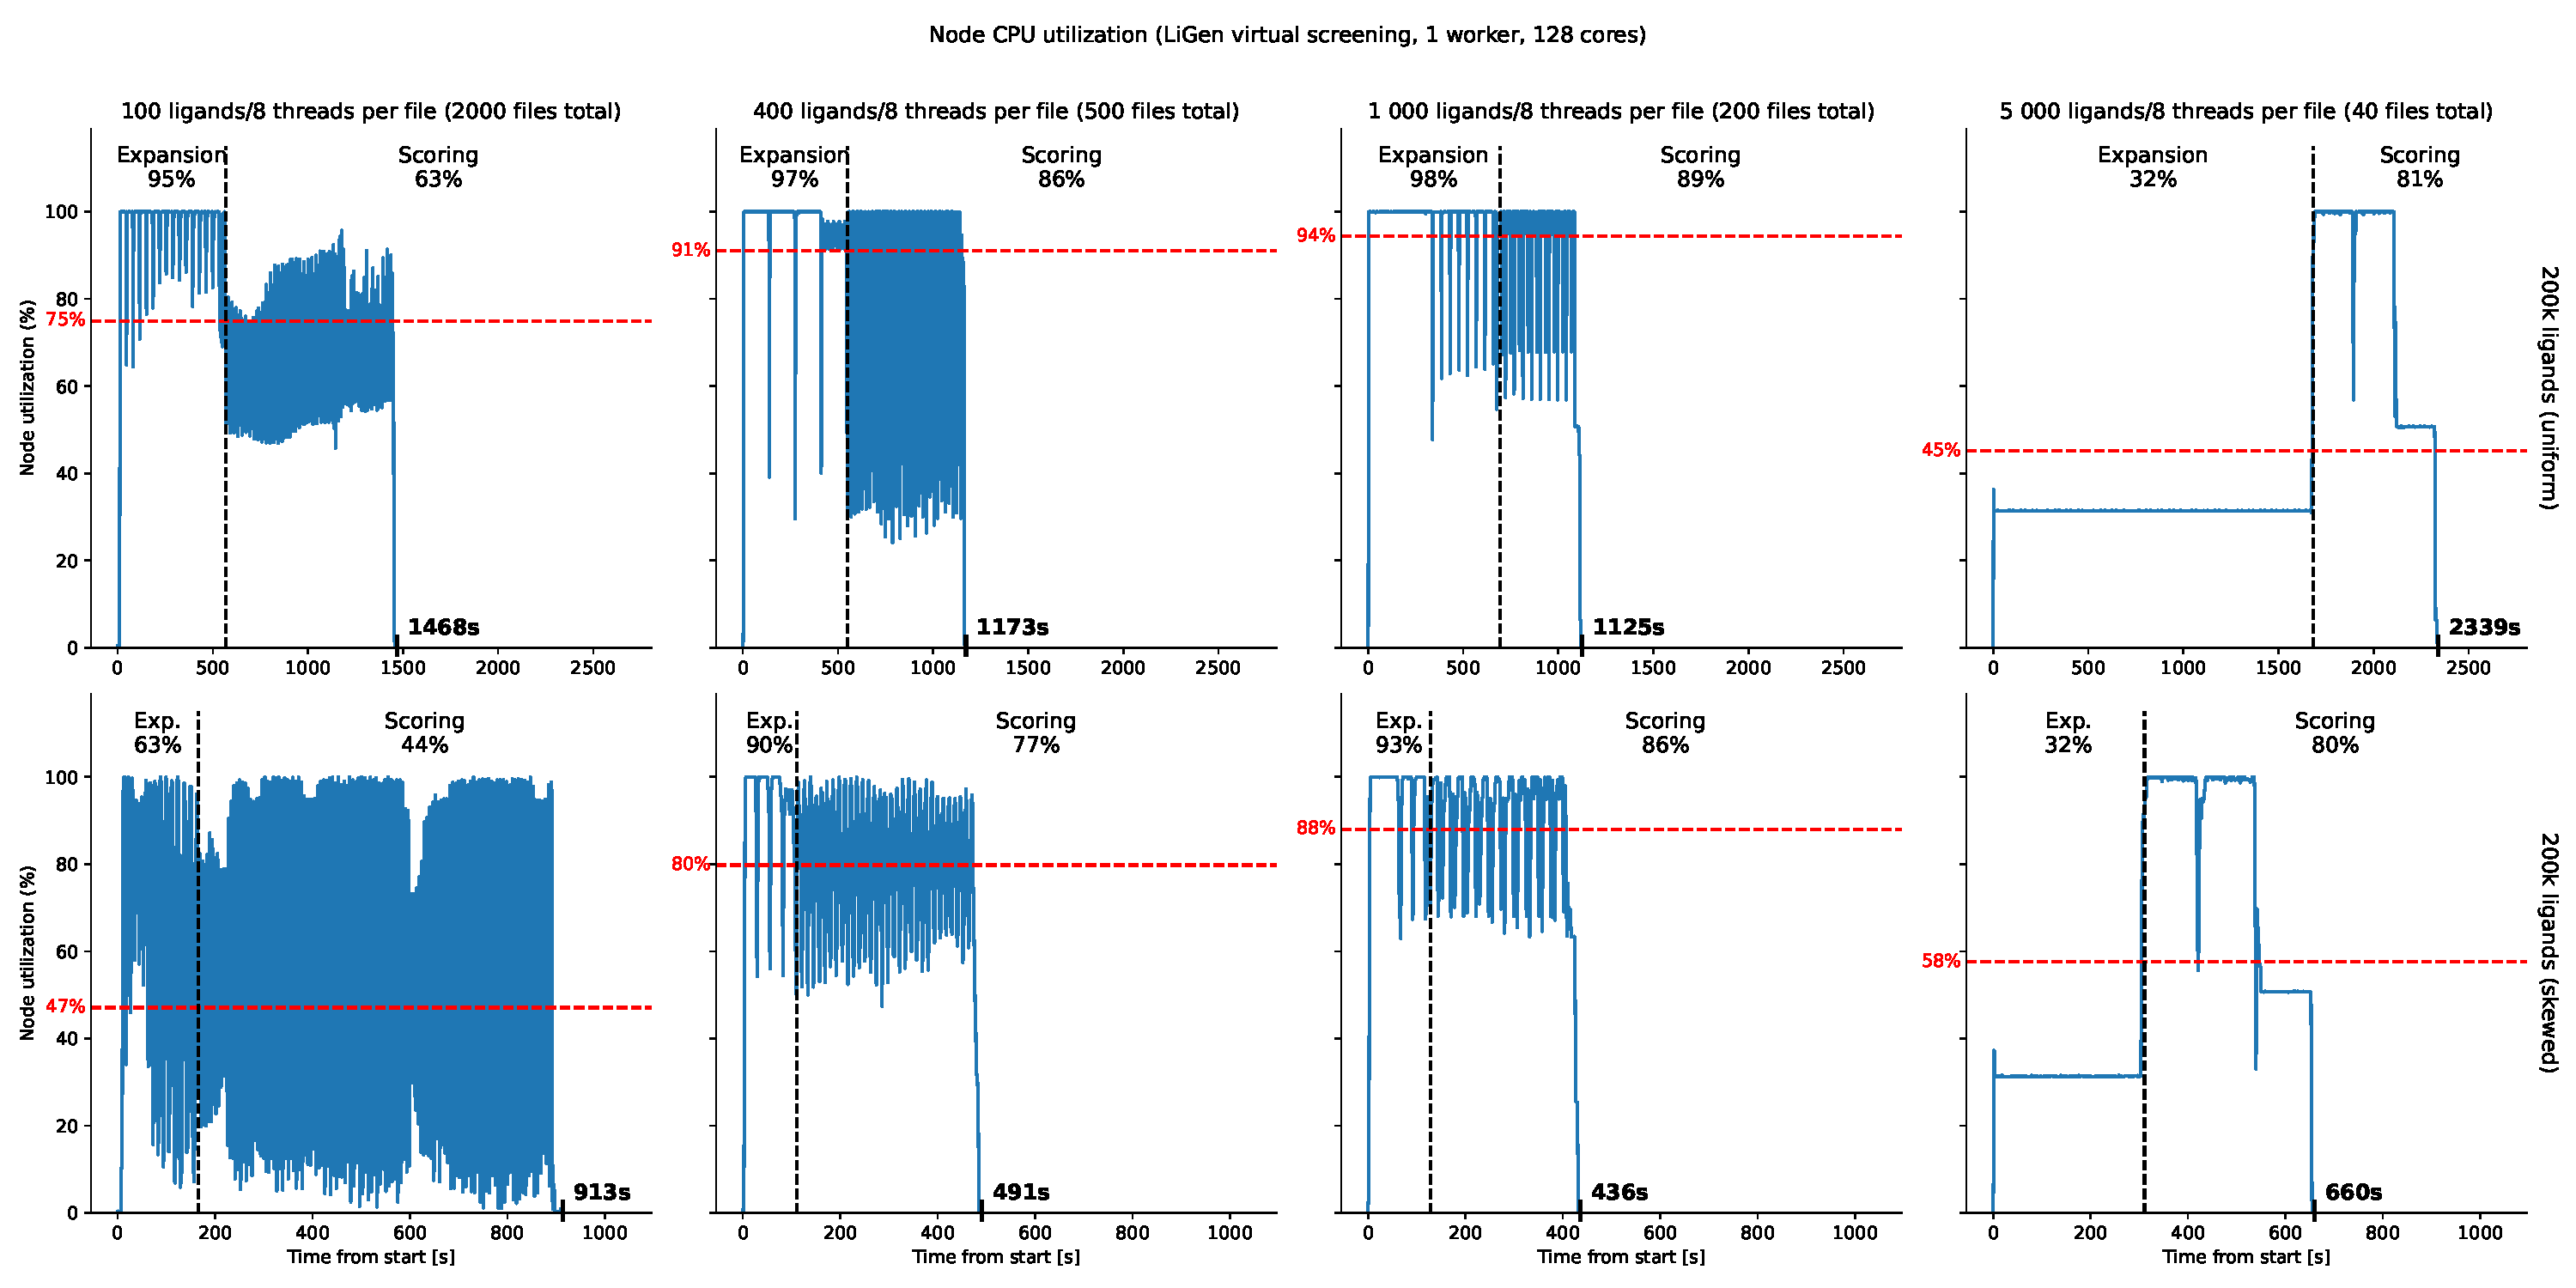
\includegraphics[width=\textwidth]{imgs/hq/charts/ligen-aggregation-utilization}
	\caption{Achieved hardware utilization of the LiGen virtual screening workflow}
	\label{fig:hq-ligen-utilization}
\end{figure}

We can see that the parameter affecting the number of ligands per file has a significant effect on
the resulting makespan; using too few or too many ligands results in a longer execution. As
expected, the expansion section needs enough tasks to saturate the available cores, because it is
single-threaded. For $5000$ ligands per file (the rightmost column), the total
number of expansion tasks is only $40$, therefore the achieved utilization (for
both input files) is around $32\%$, which corresponds to using only
$40$ out of the $128$ available cores. With more than
$128$ files available, the utilization approaches $100\%$ for the
uniform input. For the skewed input file, the utilization for the expansion section is generally
worse. With $100$ ligands per file, it is reduced significantly; unlike with the
uniform input, some of the files were expanded much quicker than others, which led to more load
imbalance.

The scoring part is internally parallel and uses all $8$ assigned cores,
therefore it does not have to be divided into so many tasks; we can see that even with only
$40$ files, it achieves around $80\%$ utilization for both
input workloads. In fact, with too many files, we can see the overhead associated with the serial
part of scoring (which needs to be performed for each file separately) starts to dominate; even
with the uniform workload, the \gls{cpu} utilization of the scoring section with
$2000$ files reaches only around $63\%$ with the uniform input
and just $44\%$ with the skewed input.

The two configurations in the middle present a sort of a sweet spot; especially with
$1000$ ligands per file, the total average utilization for both workloads is at or
above $88\%$. However, it should be noted that the best configuration will change
based on the number of used workers. This can be observed in~\Autoref{fig:hq-ligen-scalability}, which shows
how does the workflow scale up to $4$ workers ($512$ cores).
The horizontal axis shows the number of workers and the vertical axis shows the duration of the
executed task graph. We can see that with $4$ workers, the configuration with
$400$ ligands per task starts to beat the configuration with
$1000$ ligands per task, simply because the latter configuration is not able to
provide enough parallelism (tasks) to make efficient use of all the available hardware resources.
In general, \hyperqueue{} is able to reduce the makespan with additional workers being
added for all four tested configurations.

\begin{figure}[h]
	\centering
	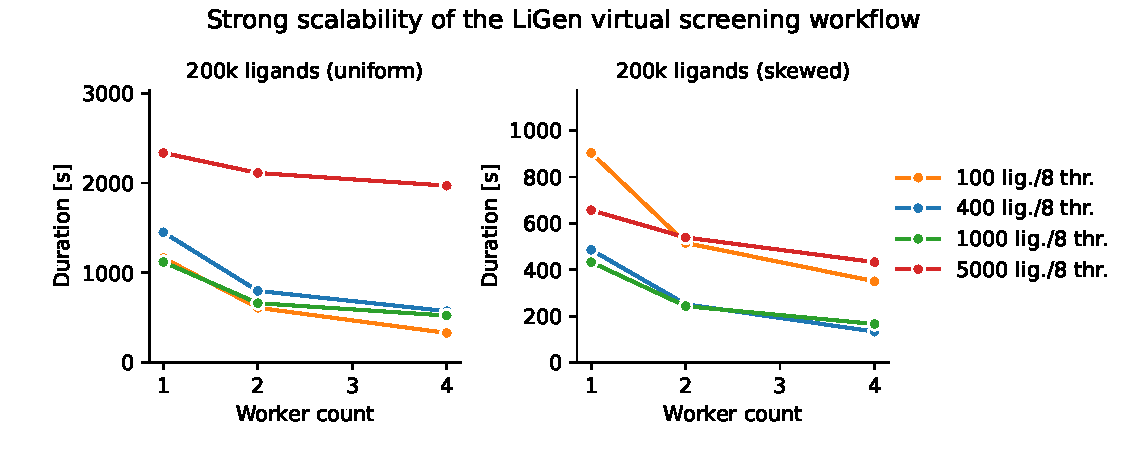
\includegraphics[width=0.8\textwidth]{imgs/hq/charts/ligen-aggregation-scalability}
	\caption{Scalability of the LiGen virtual screening workflow}
	\label{fig:hq-ligen-scalability}
\end{figure}

We can see that even when the overhead of the task runtime does not get in the way, it might be
necessary to tune the number of tasks for some workflows in order to achieve optimal performance.

\subsection{Automatic allocation}
\label{sec:hq-exp-autoalloc}
This experiment evaluates the ability of the automatic allocator to scale computational resources
both up and down in reaction to computational load. The LiGen virtual screening workflow was
executed using $16$ ligands per file and $8$ threads per
file on an input file containing $24$ thousand ligands, with a skewed
distribution of ligands. No workers were explicitly allocated for this experiment; instead, the
automatic allocator was configured to submit allocations that would start a worker. The maximum
number of workers was set to $4$, and the wall-time (the maximum duration) of
the allocations was set to $1$ minute. This very short wall-time was chosen
simply to make the benchmark run shorter, and to simulate the situation where an allocation ends in
the midst of a task graph being computed. The experiment was performed with two configurations for
the \emph{idle timeout} duration, which decides after what time a worker (and its allocation)
shuts down when it is fully idle. Each configuration was executed a single time.

\begin{figure}[h]
	\centering
	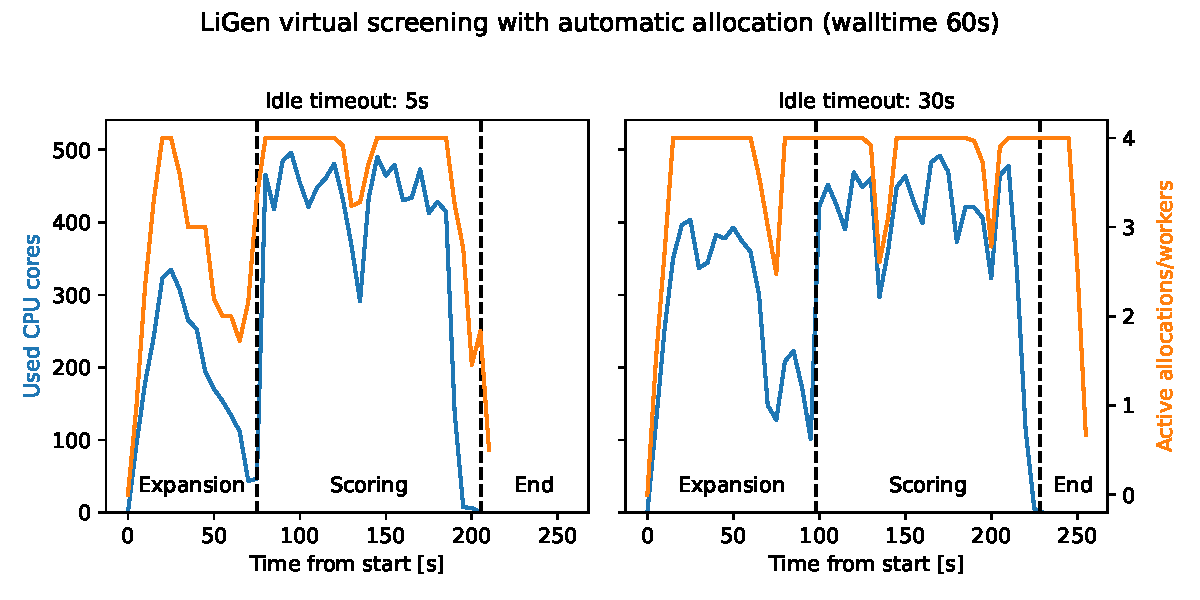
\includegraphics[width=0.8\textwidth]{imgs/hq/charts/ligen-autoalloc-stats}
	\caption{Scaling of allocations using the automatic allocator}
	\label{fig:hq-ligen-autoalloc}
\end{figure}

We can observe the result of the experiment in~\Autoref{fig:hq-ligen-autoalloc}. The horizontal axis shows
the progress of the computation. The left vertical axis and the blue line shows the number of cores
used for executing tasks (calculated as the number of running tasks times cores required per task).
The right vertical axis and the orange line shows the number of active allocations and workers,
since each allocation executed exactly one worker. The dashed vertical lines show individual
sections of the computation; expansion of ligands, scoring of expanded ligands and an
\emph{End} section, where the task graph was already computed, and the idle
allocations were waiting for the idle timeout to be applied. Note that when we benchmark automatic
allocation, the allocation manager and the global state of the cluster have a significant influence
on the time allocations spend waiting to be executed, and thus also on the total makespan of the
executed task graph; therefore, the makespans of these two executions cannot be directly compared.

We can see that allocations were dynamically submitted in response to tasks that needed workers to
execute and that new allocations were quickly created in response to previous allocations ending.
As you may recall, the wall-time was set to only one minute, after which each allocation ended,
which causes the periodic drops in active allocations in both charts. In the left chart, we can see
the results for idle timeout being configured to \SI{5}{\second}. We can observe that in
this case, the allocations are scaled down during the expansion part of the workflow, as not that
many resources are required towards the end of expansion. Furthermore, towards the end of the
computation, the number of allocations is being scaled down even before the task graph has finished
computing. In the right chart, where the idle timeout is much longer (\SI{30}{\second}), the
allocations are active for the whole duration of the task graph execution, except for short periods
of time where new allocations have to be spawned due to wall-time being exhausted. All four
allocations are also active up until the very end of the task graph computation, which results in
more allocation time being wasted.

With idle timeout \SI{5}{\second}, the workflow has consumed $682$
node-seconds of allocation time, while with idle timeout \SI{30}{\second}, it has consumed
$916$ node-seconds. This shows that it is crucial to configure the idle timeout
properly to avoid wasting allocation time. By default, \hyperqueue{} uses a wall-time of
$1$ hour and an idle timeout of $5$ minutes, which
corresponds to the same wall-time/idle-timeout ratio as the benchmarked configuration with an idle
timeout of \SI{5}{\second}.

\section{Comparison with other task runtimes}
\label{hq:related-work}
\Autoref{ch:sota} has described several existing task runtimes and their ability to cope
with the mentioned challenges that affect task graph execution on \gls{hpc} clusters.
Even within the particular area of task-based programming that was specified
in~\Autoref{ch:distributed-computing}, there are dozens of tools designed for executing some kind of task
graph, whose features and target use-cases partially overlap with \hyperqueue{}. We will
focus on a smaller subset of task runtimes that enable performing some form of meta-scheduling on
top of allocation managers and can therefore be more directly compared with
\hyperqueue{}. Several representatives of these tools will be mentioned in this section.

It should be noted that when comparing task runtimes, we compare not only the inherent properties
of their design and programming model (such as how do they specify dependencies or manage resource
requirements), but also their implementation details (such as what runtime dependencies are
necessary to deploy the task runtime). As was shown in~\Autoref{subsec:estee-schedulers}
and~\Autoref{sec:rsds-dask-overhead-analysis}, implementation details are crucial; they significantly affect both the
efficiency and scalability of the task runtime, and they also dictate how easy it is to use and
deploy it. We thus consider it important to compare actual implementations, rather than only
theoretical designs without any implementation available.

% !{\kern1em} - space
% @{} - remove space
%    \begin{tabular}{@{}lc GG !{\kern1em} GGG !{\kern1em} GG@{}}
%    \multicolumn{3}{c|}{\makecell{Task\\interfaces}} &
%    \multicolumn{p{4em}}{c|}{Task\newline{}interfaces} &
% https://stackoverflow.com/questions/1357798/how-to-center-cell-contents-of-a-latex-table-whose-columns-have-fixed-widths

% Inspiration taken from https://tex.stackexchange.com/a/377651/95679
% tasks unrelated to allocations
% map tasks to allocations
% tasks pinned to a specific queue
% task graph partitioning
% load balancing
% generic workers - Parsl no, Merlin no
% auto-allocation
% fault-tolerance - automatic, manual

% Manual task graph partitioning
\newcommand*\manualmap{\LEFTcircle}
% Automatic task graph partitioning
\newcommand*\automaticmap{\CIRCLE}
% Manual fault tolerance
\newcommand*\manualft{\LEFTcircle}
% Automatic fault tolerance
\newcommand*\automaticft{\CIRCLE}

% \begin{noindent}
\begin{table}[h]
%	\aboverulesep=0ex
%	\belowrulesep=0ex
\footnotesize
\newcommand*\rot[1]{\footnotesize\hbox to1em{\hss\rotatebox[origin=br]{-90}{#1}}}
\newcommand*\rotheading[1]{\footnotesize\hbox to1em{\hss\rotatebox[origin=br]{-60}{#1}}}
\newcommand*\feature[1]{\ifcase#1 -\or\LEFTcircle\or\CIRCLE\fi}
\newcommand*\f[3]{\feature#1&\feature#2&\feature#3}
\makeatletter
\newcommand*\ex[9]{#1\tnote{#2}&#3&%
\f#4&\f#5&\f#6&\f#7&\f#8&\f#9&\expandafter\f\@firstofone
}
% Features
\newcommand*\yes{\faThumbsOUp}
%	\newcommand*\no{\faThumbsODown}
\newcommand*\no{-}
\newcommand*\partially{\faThumbsOUp}
% CLI for submitting tasks
\newcommand*\cli{C}
% Workflow files for submitting tasks
\newcommand*\workflowfile{W}
% Python API for submitting tasks
\newcommand*\pythonapi{P}
% Requires Python
\newcommand*\python{Python}
\makeatother
\newcolumntype{A}{c@{}c}
\newcolumntype{B}{c@{}c@{}c}
\newcolumntype{C}{c@{}c@{}c@{}c}
\begin{threeparttable}
\begin{tabular}{|l|C|A|A|B|C|A|l|}
\multicolumn{1}{c}{Task runtime} &
\multicolumn{4}{c}{\rotheading{Task interfaces}} &
\multicolumn{2}{c}{\rotheading{Task dependencies}} &
\multicolumn{2}{c}{\rotheading{Fault tolerance}} &
\multicolumn{3}{c}{\rotheading{Meta-scheduling}} &
\multicolumn{4}{c}{Resources} &
\multicolumn{2}{c}{\rotheading{Data transfers}} &
\multicolumn{1}{c}{Deployment}\\
\midrule
& % tool
\rot{CLI} & \rot{Workflow file} & \rot{Python API} & \rot{Dynamic task graphs} & % interfaces
\rot{Explicit} & \rot{Inferred from files} & % dependencies
\rot{Worker failure} & \rot{Server failure} & % fault tolerance
\rot{Graph partitioning} &
\rot{Automatic allocation} & \rot{Generic workers} & % meta-scheduling
\rot{Basic (CPU/GPU)} & \rot{Generic resources} & \rot{Resource pools} &
\rot{Multi-node tasks} & %resources
\rot{Directly between tasks} & \rot{Output streaming} & % data transfers
Runtime dependencies \\ % deployment
\midrule
\gnuparallel{}\hfill\cite{parallel} & \yes & \no & \no & \no & \no & \no & \manualft & \no & \no & \no & \no & \no & \no & \no & \no & \no & \yes & Perl \\
%	\midrule
\hypershell{}\hfill\cite{hypershell} & \yes & \no & \yes & \no & \no & \no & \automaticft & \yes & \manualmap & \yes & \no & \no & \no & \no & \no & \no & \yes & \python \\
%	\midrule
\dask{}\hfill\cite{dask} & \no & \no & \yes & \yes & \yes & \no &
\automaticft & \no & \automaticmap\textsuperscript{\dag} & \yes\textsuperscript{\dag} & \yes & \yes & \yes & \no & \no & \yes & \yes & \python \\
%	\midrule
\ray{}\hfill\cite{ray} & \no & \no & \yes & \yes & \yes & \no & \automaticft & \yes
\textsuperscript{*} & \automaticmap & \no & \yes & \yes & \yes & \no & \no & \yes & \partially & \python \\
%	\midrule
\parsl{}\hfill\cite{parsl} & \no & \no & \yes & \yes & \yes & \no & \automaticft &
\no & \automaticmap & \yes & \no & \yes & \no & \no & \yes & \yes & \no & \python \\
%	\midrule
\pycompss{}\hfill\cite{pycompss} & \yes & \no & \yes & \yes & \yes & \no & \automaticft &
\yes\textsuperscript{*} & \manualmap & \no & \no & \yes & \no & \no & \yes & \yes & \yes & \python, Java \\
%	\midrule
\pegasus{}\hfill\cite{pegasus} & \no & \yes & \yes & \no & \yes & \yes & \automaticft &
\yes & \manualmap & \no & \no & \yes & \no & \no & \no & \no & \yes & \python, Java,
HTCondor~\cite{htcondor} \\
%	\midrule
\balsam{}\hfill\cite{balsam} & \no & \no & \yes & \yes & \yes & \no & \automaticft &
\yes & \automaticmap & \yes & \yes & \yes & \no & \no & \yes & \yes & \no & \python,
PostgreSQL \\
%	\midrule
\autosubmit{}\hfill\cite{autosubmit} & \no & \yes & \no & \no & \yes & \no & \automaticft &
\yes & \manualmap & \yes & \no & \yes & \no & \no & \yes & \no & \no & \python \\
%	\midrule
\fireworks{}\hfill\cite{fireworks} & \no & \yes & \yes & \yes & \yes & \no & \manualft &
\yes & \automaticmap & \yes & \yes & \no & \no & \no & \no & \no & \no & \python, MongoDB \\
%	\midrule
\merlin{}\hfill\cite{merlin} & \no & \yes & \no & \no & \yes & \no & \manualft &
\yes & \automaticmap & \no & \no & \yes & \no & \no & \yes & \no & \no & \python, RabbitMQ/Redis \\
%	\midrule
\snakemake{}\hfill\cite{snakemake} & \no & \yes & \yes & \no & \no & \yes & \automaticft &
\no & \manualmap & \yes\textsuperscript{\dag} & \no & \yes & \yes & \no & \yes & \no & \no & \python \\[2mm]
%	\midrule
\hyperqueue{}\hfill\cite{hyperqueue} & \yes & \yes & \yes & \yes & \yes & \no & \automaticft &
\yes & \automaticmap & \yes & \yes & \yes & \yes & \yes & \yes & \no & \yes & \\
\bottomrule
\end{tabular}
\begin{tablenotes}
\centering
\item \yes{} supported; \no{} not supported; \automaticmap{} automatic; \manualmap{} manual;
\item \textsuperscript{\dag}with an external plugin; \textsuperscript{*}with additional
runtime dependencies
\end{tablenotes}
\caption{Comparison of task runtimes}
\label{tab:hq-tools-comparison}
\end{threeparttable}
\end{table}
% \end{noindent}

\Autoref{tab:hq-tools-comparison} provides a high-level comparison of \hyperqueue{} and twelve
other task runtimes. It should be noted that there are also many important properties that are not
mentioned in this table; it primarily compares meta-scheduling aspects described in this chapter
and other features related to challenges described in~\Autoref{ch:sota}. Furthermore, there
is no single universally best task runtime; each one has a different programming model, a different
set of features, and makes various trade-offs based on which use-cases it was primarily designed
for.

The first section of the table, \emph{Task interfaces}, shows which interfaces can be used to
submit tasks and if they support modifying task graphs dynamically. \gls{cli}
specifies that tasks can be submitted from the command-line, \emph{Workflow file} specifies that
task graphs can be defined using e.g.\ \gls{yaml} or \gls{toml} files and
\emph{Python \gls{api}} marks runtimes that provide the option to specify tasks using Python. Note
that the \gls{cli} column indicates that tasks and task graphs can be actually
defined and submitted using the command-line, without requiring additional input files, not just
that the runtime provides some form of a \gls{cli} (which is true for most of the runtimes). The last column,
\emph{Dynamic task graphs}, states whether the task runtime supports adding to existing submitted task
graphs dynamically, which is useful for expressing iterative workflows.

Most evaluated task runtimes provide a Python \gls{api}, as it enables the most
general way of defining task graphs. However, it is relatively rare for other tools to offer a
comprehensive \gls{cli} that could be used to submit simple task graphs without the
need to implement a script using (an imperative) programming language. \merlin{} and
\autosubmit{} only allow defining task graphs using workflow files, which can also be
quite verbose for simple use-cases. \hyperqueue{} offers both a terminal interface for
simple use-cases, and a Python \gls{api} for more complex task graphs. It also
supports workflow files.

The second section, \emph{Task dependencies}, marks the ability to express dependencies between
tasks. \emph{Explicit} dependencies are described by the user in the task graph definition,
usually by mentioning a set of task identifiers on which a given task depends.
\gnuparallel{} and \hypershell{} do not allow specifying task dependencies, as
they are designed mostly for scenarios where users simply need to execute a large number of tasks
in parallel. Most other tools allow expressing dependencies between tasks explicitly.
\pegasus{} and \snakemake{} are also able to infer dependencies
automatically based on input/output files consumed/produced by the individual tasks. For
\snakemake{}, it is the only way to express dependencies, which can limit performance
for task graphs with many tasks, as every dependency necessitates the creation of a file on a
filesystem.

The third section, \emph{Fault tolerance} describes what happens when after a worker or a server
failure. Task runtimes that can automatically restart tasks after a worker failure are marked with
\automaticft, those that require user action to recompute failed tasks are marked with \manualft.
All the evaluated task runtimes provide support for at least some kind of resilience against worker
failures; it is a truly fundamental feature without which it would be infeasible to execute task
graphs. To be resilient against server failures, the task runtime should be able to restore the
state of already computed tasks, and all the submitted task graphs, when the task submission
command or the main server/scheduler component crashes (e.g.\ when it is executed on a login node
that shuts down). This property is very useful for avoiding unnecessary re-execution of
long-running task graphs. Resilience against server failures is supported so ubiquitously, although
is is still a rather common feature. However, most task runtimes require an external service or a
database instance to implement server persistence, which can complicate their deployment.

The fourth section, \emph{Meta-scheduling}, specifies three properties related to executing tasks
on top of allocations and general scheduling capabilities. The following list describes the
individual columns:

\begin{description}[wide=0pt]
	\item[Graph partitioning] states whether the task runtime can assign tasks to allocations fully automatically (\automaticmap)
		or if users have to partition tasks into subgroups manually (\manualmap). As already mentioned
		in~\Autoref{ch:sota}, tools such as \pegasus{}, \autosubmit{} or
		\snakemake{} require users to manually specify how should tasks be grouped into
		allocations, which requires more work from the user and can limit hardware utilization. Other task
		runtimes, such as \dask{} or \balsam{}, are able to fully
		automatically assign tasks to allocations without any intervention from the user, same as
		\hyperqueue{}.

	\item[Automatic allocation] highlights task runtimes that are able to automatically submit \emph{\gls{hpc} allocations}. There are
		various levels of support for this feature. \snakemake{} or \autosubmit{}
		simply submit allocations that are designed for executing a specific task (or a group of tasks),
		while other task runtimes, such as \dask{}, \balsam{} or
		\hyperqueue{}, submit allocations dynamically, based on the current computational load
		and task state; these allocations start a generic worker that is not tied to any specific task or a
		subset of tasks. Unlike \hyperqueue{}, \dask{} and
		\balsam{} support configuring only a single allocation manager queue into which new
		allocations can be submitted.

	\item[Generic workers] states whether the task runtime supports provisioning of generic workers that can execute any tasks
		whose resource requirements are compatible with it, without requiring users to preconfigure workers
		statically for a specific subset of tasks (which makes load balancing less flexible).
		\merlin{} requires preconfiguring queues that are used for executing specific tasks
		(such as a task that requires exactly two nodes or sixteen \gls{cpu} cores to
		execute). A similar rigid approach is used by \parsl{}. On the other hand,
		\dask{} or \hyperqueue{} make worker spawning very easy, using a single
		generic command, since their workers are not tied to any specific task.
\end{description}

The following section, \emph{Resources}, deals with resource management. It shows which task
runtimes are only able to specify basic (such as \gls{cpu}, \gls{gpu}
or memory) task resource requirements and which are able to attach fully generic and arbitrary
requirements to each task. Support for arbitrary resource requirements (and thus heterogeneous
clusters) is not very common, apart from \hyperqueue{}, only \dask{},
\ray{} and \snakemake{} allow users to define their own resource kinds
that are then used in task scheduling. The \emph{Resource pools} column describes the ability to
specify (and take into account during scheduling) complex resource requirements, such as specifying
relationships between resources (i.e.\ two cores in the same \gls{numa} node),
fractional resources or resource variants. This functionality is unique to \hyperqueue{}.
The \emph{Multi-node} column shows which programming models enable describing multi-node
tasks. Note that the table only treats this feature as supported in task runtimes that provide the
ability to assign the number of nodes \emph{per-task}, not just per task graph or per
allocation. We can see that \snakemake{} is the only task runtime apart from
\hyperqueue{} that supports both arbitrary resource requirements and multi-node tasks.

The penultimate section, \emph{Data transfers}, states whether it is possible to exchange data
outputs between tasks directly over the network, without going through the filesystem
(\emph{Directly between tasks}) and if the task runtime offers the ability to stream standard (error)
output of tasks over the network to overcome distributed filesystem limitations
(\emph{Output streaming}). Direct data transfer of task outputs is supported by Python-first task
runtimes, such as \dask{} or \ray{}. It is not supported by
\hyperqueue{}.

The last section, \emph{Deployment}, specifies which runtime dependencies and external
services have to be available in order to use the task runtime. We can see that almost all
evaluated task runtimes require Python, as it is a very popular technology for working with tasks.
Some task runtimes, such as \merlin{} or \fireworks{}, additionally
require an external service for managing persistence or task assignments, these can be challenging
to deploy on \gls{hpc} clusters. Note that this column specifies the
\emph{required} runtime dependencies, which are necessary for the task runtime to function.
It does not mention optional dependencies; for example, \hyperqueue{}'s Python
\gls{api} of course also requires a Python interpreter, but \hyperqueue{}
itself can operate without it.

Even though several existing task runtimes also leverage meta-scheduling, they do not offer a
holistic set of features that would help resolve the most pressing issues of task graph execution
on heterogeneous supercomputers all at once. Some of them are not focused primarily on
\gls{hpc} problems, while others tie tasks to allocations too strongly, which reduces
load-balancing opportunities and limits local prototyping. Some of them also require runtime
dependencies that complicate their deployment.

\hyperqueue{} treats \gls{hpc} as a first-class citizen, and provides a
unified set of features that help task graph authors execute their task graphs in an easy way on
\gls{hpc} clusters. It is also very efficient and can scale to a large number of
hardware resources, while being trivial to deploy. Furthermore, \hyperqueue{} provides
unique resource scheduling features in the form of fractional resources and primarily resource
variants, which can help improve the achieved hardware utilization. On the other hand, in the
current version, its programming model does not yet integrate direct data transfers between tasks,
which can be limiting for use-cases that require this functionality.

%The individual task runtimes will be briefly discussed and compared with \hyperqueue{}
%below.
%
%\subsubsection*{\gnuparallel}
%\gnuparallel~\cite{parallel} is a command-line utility for executing many tasks in
%parallel on a set of computational nodes. It does not offer many advanced task runtime features,
%but it does one thing well; it enables a parallelized and even distributed execution of a set of
%programs with a single command invocation. \hyperqueue{} takes inspiration from this
%approach, as it offers a \gls{cli} that can be used to execute task graphs with many
%tasks and complex resource requirements with a single command.
%
%\subsubsection*{\hypershell}
%\hypershell~\cite{hypershell} is also primarily designed for
%executing many homogeneous tasks using the command-line. It does introduce several useful features
%on top of \gnuparallel, such as automatic task re-execution when a task fails and storing the task
%state in a database, so that users can observe the history of executed task graphs. It also
%provides a simple autoscaling functionality that automatically submits allocations. However, tasks
%in \hypershell are strictly tied to allocations; by default, one task is submitted in a single
%allocation. It does provide the option to \emph{bundle} several tasks together, but users
%have to specify the maximum bundle size explicitly, which makes load balancing inflexible.
%\hypershell does not support task dependencies; therefore, it cannot be used to execute general
%task graphs.
%
%\subsubsection*{\dask}
%\dask~\cite{dask} was already extensively decribed in~\Autoref{sec:rsds-dask}. It is a
%distributed task runtime written in Python, which allows parallelizing and distributing Python code
%in an easy way. \dask{} offers a low-level \gls{api} for building
%task graphs explicitly from Python function calls, however one of its most powerful features is the
%ability to parallelize \texttt{numpy} and \texttt{pandas} code by automatically
%transforming it to a task graph. \dask{} is very flexible in terms of load
%balancing and it is also very easy to use. With the use of a separate plugin called
%\textsc{Dask-JobQueue}~\cite{dask-jobqueue}, it is able to submit \gls{pbs} or
%Slurm allocations and also automatically scale them according to computational load. However, it
%only allows using a single queue for automatic allocation, which can make it challenging to execute
%task graphs that leverage heterogeneous resources (such as both \gls{cpu} and
%\gls{gpu} partitions of a cluster).
%
%Its resource requirement support is not as advanced as in \hyperqueue{} and it does not
%support multi-node tasks. Crucially, its performance is severely limited by its implementation
%language (Python), as we have shown in~\Autoref{dask:evaluation}; for \gls{hpc}-scale
%workflows, \hyperqueue{} easily outperforms it, which was further demonstrated
%in~\Autoref{sec:hq-exp-dask}.
%
%\subsubsection*{\ray}
%\ray~\cite{ray} is a distributed task runtime primarily aimed at parallelizing the
%training and inference of machine learning models in Python. \ray{} uses a
%relatively unique architecture, which leverages distributed scheduling; not all task submission and
%scheduling decisions need to go through a central location, unlike most other task runtimes
%mentioned in this section, including \hyperqueue{}. This allows it to scale to an
%enormous amount of resources, millions of tasks and thousands of nodes. However, in order to enable
%this level of scalability, the workflow itself has to be implemented in a way where tasks submit
%new tasks from worker nodes dynamically. Therefore, batch computing use-cases that simply want to
%execute a pre-determined workflow will not be able to achieve such high performance.
%
%Same as \dask{}, it offers basic resource requirements, but does not allow
%expressing multi-node tasks. In contrast to \dask{}, it is internally implemented
%in \texttt{C++}, which allows introduces much less overhead than Python.
%\ray{} provides autoscaling functionality, but it does not support Slurm or other
%\gls{hpc} allocation managers. In general, it is not specialized for
%\gls{hpc} idiosyncrasies nor for executing arbitrary task graphs; even though it has
%a low-level interface for creating tasks through Python functions, it primarily focuses on
%generating task graphs automatically from high-level descriptions of machine learning pipelines.
%
%\subsubsection*{\parsl}
%\parsl~\cite{parsl} is another representative of a Python-oriented task runtime. It
%allows
%defining tasks that represent either Python function calls or command-line application
%invocations using Python. Computational resources in \parsl are configured through a
%\emph{block}, a set of preconfigured resources (nodes) designed for executing specific
%kinds of tasks. In addition to blocks, users also have to specify \emph{launchers}, which
%determine how will be each task executed (e.g.\ using a Slurm or an \gls{mpi}
%execution command), and also an \emph{executore}, which controls how will tasks be
%scheduled, batched into allocations and if the execution will support fault tolerance. While these
%options let users specify how will be their task graph executed on a very granular level, it
%requires them to tune this configuration per task graph or target cluster, and the whole system is
%relatively complex. This is in contrast to \hyperqueue, which has a fully general resource
%management model that does not require users to configure anything; tasks are automatically
%load-balanced across all available workers regardless of allocations, and workers do not have to be
%preconfigured for specific tasks.
%
%\parsl has basic support for resource requirements, but does not allow
%creating custom user-specified resource types. It also allows specifying the number of nodes
%assigned to a task, however such tasks have to be executed within a single block; \parsl
%is not able to execute multi-node tasks across different blocks or allocations.
%
%\subsubsection*{\pycompss}
%\pycompss~\cite{pycompss} is a Python interface for executing task graphs on top of the
%COMPSs distributed system. It allows defining arbitrary task graphs and has comprehensive support
%for multi-node tasks and basic resource requirements, but it does not allow users to define custom
%resource requirements. In terms of scheduling, it implements several simple scheduling algorithms;
%users can select which one should be used. Assignment of tasks to allocations is performed in a
%manual way; users enqueue a task graph (an \emph{application}), which is then fully executed
%once that allocation is started. COMPSs provides basic support for automatic allocation that can
%react to computational load dynamically. However, it can only add or remove nodes from a primary
%allocation that is always tied to the execution of a single application; it does not provide fully
%flexible load balancing. \pycompss is slightly more challenging to deploy than most of the other
%mentioned task runtimes, since it also requires a Java runtime environment in addition to a Python
%interpreter.
%
%\subsubsection*{\pegasus}
%\pegasus~\cite{pegasus} is a very general workflow management system that can execute
%workflows on a wide range of clusters, from \gls{hpc} to cloud. It provides support
%for various additional features that have not been examined in this thesis, such as data provenance
%or advanced file management and staging. Its workflows are usually defined using workflow files,
%which enable specifying dependencies both explicitly or by inferring them from input/output files
%of tasks. It also supports basic resource requirements, but does not allow assigning custom
%resources to tasks or workers, and does not support multi-node tasks. By default, it maps each task
%to a single allocation, but it also allows users to \emph{cluster} tasks together using
%one of several predefined modes. However, users have to configure this clustering manually, it is
%not performed fully automatically like in \hyperqueue{}.
%
%In terms of deployment, it has the most complex runtime dependencies out of the compared task
%runtimes, as it requires not only a Python interpreter and a Java runtime environment, but also the
%HTCondor~\cite{htcondor} workload management system, which can be non-trivial to install on
%an \gls{hpc} cluster. \pegasus{} delegates some of its functionality to
%HTCondor and requires a configured instance of HTCondor before it can execute workflows on a
%cluster.
%
%\subsubsection*{\balsam}
%\balsam~\cite{balsam} is a task runtime for executing workflows defined using Python on
%\gls{hpc} clusters. It uses a similar fully flexible method for mapping tasks to
%allocations as \hyperqueue{}, including automatic allocation; however, it is limited to a
%single allocation queue, similarly as in \dask{}. It supports multi-node tasks,
%although users have to statically preconfigure workers to either execute single-node or multi-node
%tasks. It does not allow specifying custom resource requirements (nor more advanced resource
%management offered by \hyperqueue{}, such as resource variants), which limits its
%usability for heterogeneous clusters.
%
%The \balsam{} server requires access to a PostgreSQL database instance, which makes
%its deployment slightly more challenging than some other tools that do not need a database or that
%can use an embedded database like SQLite.
%
%\subsubsection*{\autosubmit}
%\autosubmit~\cite{autosubmit} is a tool for executing workflows and experiments. It focuses
%primarily on experiment tracking, data provenance and workflow automation. In its default mode,
%each task corresponds to a single allocation, which is not ideal for short running tasks;
%\autosubmit is designed for more high-level and coarse-grained workflows. It provides a way to
%bundle multiple tasks into the same allocation using \emph{wrappers}, but same as with
%e.g.\ \pegasus{}, this has to be preconfigured statically by the user and it is not
%performed automatically. \autosubmit{} does not support custom task resource requirements
%and it also does not support direct data transfers between tasks nor output streaming.
%
%\subsubsection*{\fireworks}
%\fireworks~\cite{fireworks} is a workflow system for managing the execution of workflows on
%distributed clusters. It allows defining task graphs using either workflow files or through a
%Python \gls{api}. It supports fault-tolerant task execution, although failed tasks
%have to be re-executed manually. \fireworks{} does not seem to support any task resource
%requirements; resources can only be configured for individual allocations. Its meta-scheduling
%approach is relatively complicated; it provides several ways of mapping tasks to allocations and
%individual workers with different trade-offs, rather than providing a unified way that users would
%not have to worry about. \fireworks{} requires a MongoDB database instance to store the
%state of tasks, which again makes its deployment slightly more challenging.
%
%\subsubsection*{\merlin}
%\merlin~\cite{merlin} is a task queue system that enables execution of large workflows on
%\gls{hpc} clusters. It leverages the Celery~\cite{celery} task queue for
%distributing tasks to workers and the Maestro~\cite{maestro} workflow specification for
%defining task graphs. Tasks are submitted into separate Celery queues; whose resources need to be
%preconfigured, its load balancing is thus not fully flexible and automatic like in
%\hyperqueue{}. It also does not support automatic allocation of allocations and workers
%and also does not support custom resource requirements. Failed tasks can be automatically restarted
%if they end with a specific status code; however, if they fail because of unexpected reasons, users
%have to mark them for re-execution manually. \merlin{} requires a message broker
%backend, such as RabbitMQ or Redis, for its functionality, which makes its deployment non-trivial.
%
%\subsubsection*{\snakemake}
%\snakemake~\cite{snakemake} is a popular workflow management system for executing
%coarse-grained workflows defined using workflow files that can be extended with inline Python code.
%\snakemake{} workflows are based on files, tasks are expected to produce and consume
%files, which are also used to infer dependencies between them. This can pose an issue with a large
%number of tasks, as the created files can overload distributed filesystems; no output streaming is
%offered by the task runtime. It does enable assigning both known (e.g.\ \gls{cpu} or
%memory) and custom resource requirements to tasks, and also specify the number of nodes required
%for each task. Similarly to \pegasus{} or \autosubmit{}, it provides an
%option to \emph{cluster} multiple tasks into the same allocation, however this
%partitioning has to be specified manually by users. Other than that, it submits tasks as individual
%allocations, which is not ideal for large workflows, because it can easily overload the target
%cluster~\cite{nersc-snakemake}.

\section*{Summary}
This chapter has presented a meta-scheduling design for executing task graphs on
\gls{hpc} clusters that was built from the ground up to overcome the issues mentioned
in~\Autoref{ch:sota}. It has also introduced \hyperqueue{}, a distributed task
runtime that implements this design through an \gls{hpc} focused programming model,
which enables ergonomic execution of workflows on supercomputers. It is able to meta-schedule tasks
to provide load balancing among separate allocations, while respecting complex resource
requirements that can be arbitrarily configured separately for each task. Its automatic allocator
can submit allocations fully autonomously on behalf of the user, which further simplifies the
execution of \hyperqueue{} task graphs. It also offers both a straightforward
\gls{cli} and a Python \gls{api} for more complex use-cases, and it is
trivial to deploy on supercomputers.

The overhead and scalability of \hyperqueue{} was evaluated in various situations. The
results indicate that it consumes little resources, introduces a reasonable amount of overhead and
can scale to tens of nodes and thousands of cores. The experiments have also shown that it is more
than competitive against \dask{}, a very popular task runtime that is being
commonly used for running task graphs on distributed clusters.

Several ideas for the future improvement of \hyperqueue{} will be summarized in the final
chapter.
